\DocumentMetadata{
    lang=de,
    pdfversion=1.0,
    tagging=off
}
\documentclass[a4paper,12pt]{article}
\usepackage{fontspec}
\setmainfont{Times New Roman}
\usepackage[english,ngerman]{babel}
\usepackage{csquotes}
\usepackage{geometry}
\usepackage{booktabs}
\usepackage{tabularx}
\usepackage{graphicx}
\usepackage{float}
\usepackage{caption}
\usepackage{pdfpages}
\usepackage{needspace}
\usepackage{longtable}
\usepackage{pdflscape}
\usepackage{eso-pic}
\usepackage{fancyhdr}
\PassOptionsToPackage{hyphens}{url}
\usepackage{hyperref}
\usepackage[style=apa, backend=biber, sorting=nyt]{biblatex}
\DefineBibliographyStrings{ngerman}{%
    nodate = {o\adddot\addabbrvspace D\adddot},
}
\DeclareFieldFormat{extradate}{%
    \iffieldbibstring{labelyear}{}{\iffieldnums{labelyear}{\mknumalph{#1}}{\apashortdash\mknumalph{#1}}}%
}
\addbibresource{Quellen/BA/BA.bib}

\geometry{left=3cm,right=2.5cm,top=2.5cm,bottom=2.5cm}
\renewcommand{\baselinestretch}{1.35}\selectfont
\setlength{\parindent}{0pt}
\setlength{\parskip}{6pt}
\hypersetup{
    hidelinks,
    pdfdisplaydoctitle=true,
    pdftitle={Vom IST-Prozess zum n8n-gestützten SOLL-Prozess: Schwachstellenanalyse und prototypische Teilautomatisierung der Materialbeschaffung in einem kleinen Handwerksbetrieb},
    pdfauthor={Cedric Jon Arnhold},
    pdfsubject={Bachelorarbeit im Studiengang Wirtschaftsinformatik},
    pdfkeywords={Materialbeschaffung, Prozessautomatisierung, n8n, BPMN, Design Science, Handwerk}
}
\makeatletter
\renewcommand{\@pnumwidth}{4.2em}
\renewcommand{\@tocrmarg}{5.2em}
\def\toclevel@frontmatter{1}
\newcommand*\l@frontmatter[2]{%
    \ifnum\c@tocdepth>\m@ne
        \addpenalty{-\@highpenalty}%
        \addvspace{0.25em \@plus 0.1em}%
        \setlength\@tempdima{1.5em}%
        \begingroup
            \parindent\z@
            \rightskip\@pnumwidth
            \parfillskip-\@pnumwidth
            \leavevmode\bfseries
            \advance\leftskip\@tempdima
            \hskip-\leftskip
            #1\nobreak\hfil\nobreak
            \hb@xt@\@pnumwidth{\hss #2}\par
        \endgroup
    \fi
}
\makeatother
\urlstyle{same}
\sloppy
\setlength{\emergencystretch}{2em}
\hbadness=10000
\hfuzz=3pt
\vfuzz=3pt
\hyphenation{Angebotsvergleich Handwerksbetriebe Materialbeschaffungsprozess nachvollziehbar Klärpfade Testdaten Treffer Venkiteela}
\setlength{\textfloatsep}{8pt plus 2pt minus 2pt}
\setlength{\floatsep}{8pt plus 2pt minus 2pt}
\setlength{\intextsep}{8pt plus 2pt minus 2pt}
\setlength{\abovecaptionskip}{4pt}
\setlength{\belowcaptionskip}{0pt}
\newcommand{\LandscapePageNumbersOn}{%
    \pagestyle{empty}%
    \thispagestyle{empty}%
    \AddToShipoutPictureFG{%
        \AtPageLowerLeft{%
            \put(
                \LenToUnit{\dimexpr\paperwidth-12mm\relax},
                \LenToUnit{.5\paperheight}
            ){%
                \rotatebox{90}{\makebox[0pt][c]{\thepage}}%
            }%
        }%
    }%
}
\newcommand{\LandscapePageNumbersOff}{%
    \ClearShipoutPictureFG%
    \pagestyle{appendixpages}%
}

\newcommand{\InterviewPart}[1]{%
    \Needspace{4\baselineskip}%
    \par\bigskip\noindent{\large #1}\par\smallskip
}
\newcommand{\InterviewSpeakerLine}[2]{%
    \Needspace{3\baselineskip}%
    \par\noindent#1\hfill{\footnotesize\itshape #2}\par\nobreak
}
\newcommand{\InterviewQuestion}[2]{%
    \InterviewSpeakerLine{\textbf{A}}{#1}%
    {\small\itshape #2\par}%
}
\newcommand{\InterviewAnswer}[2]{%
    \InterviewSpeakerLine{\textbf{B}}{#1}%
    {\small #2\par}%
}
\fancypagestyle{appendixpages}{%
    \fancyhf{}%
    \renewcommand{\headrulewidth}{0pt}%
    \renewcommand{\footrulewidth}{0pt}%
    \fancyfoot[C]{\thepage}%
}
\fancypagestyle{interviewcontinuation}{%
    \fancyhf{}%
    \renewcommand{\headrulewidth}{0pt}%
    \renewcommand{\footrulewidth}{0pt}%
    \fancyfoot[L]{%
        \footnotesize
        \begin{tabular}[b]{@{}l@{}}
            A = interviewende Person\\
            B = interviewte Person
        \end{tabular}%
    }%
    \fancyfoot[C]{\thepage}%
}

\setcounter{secnumdepth}{2}
\setcounter{tocdepth}{2}
\renewcommand{\thesection}{\arabic{section}.}
\renewcommand{\thesubsection}{\thesection\arabic{subsection}.}


\begin{document}

\hypersetup{pageanchor=false}
\begingroup
\setkeys{Gin}{alt={Deckblatt der Bachelorarbeit mit Titel- und Prüfungsangaben}}
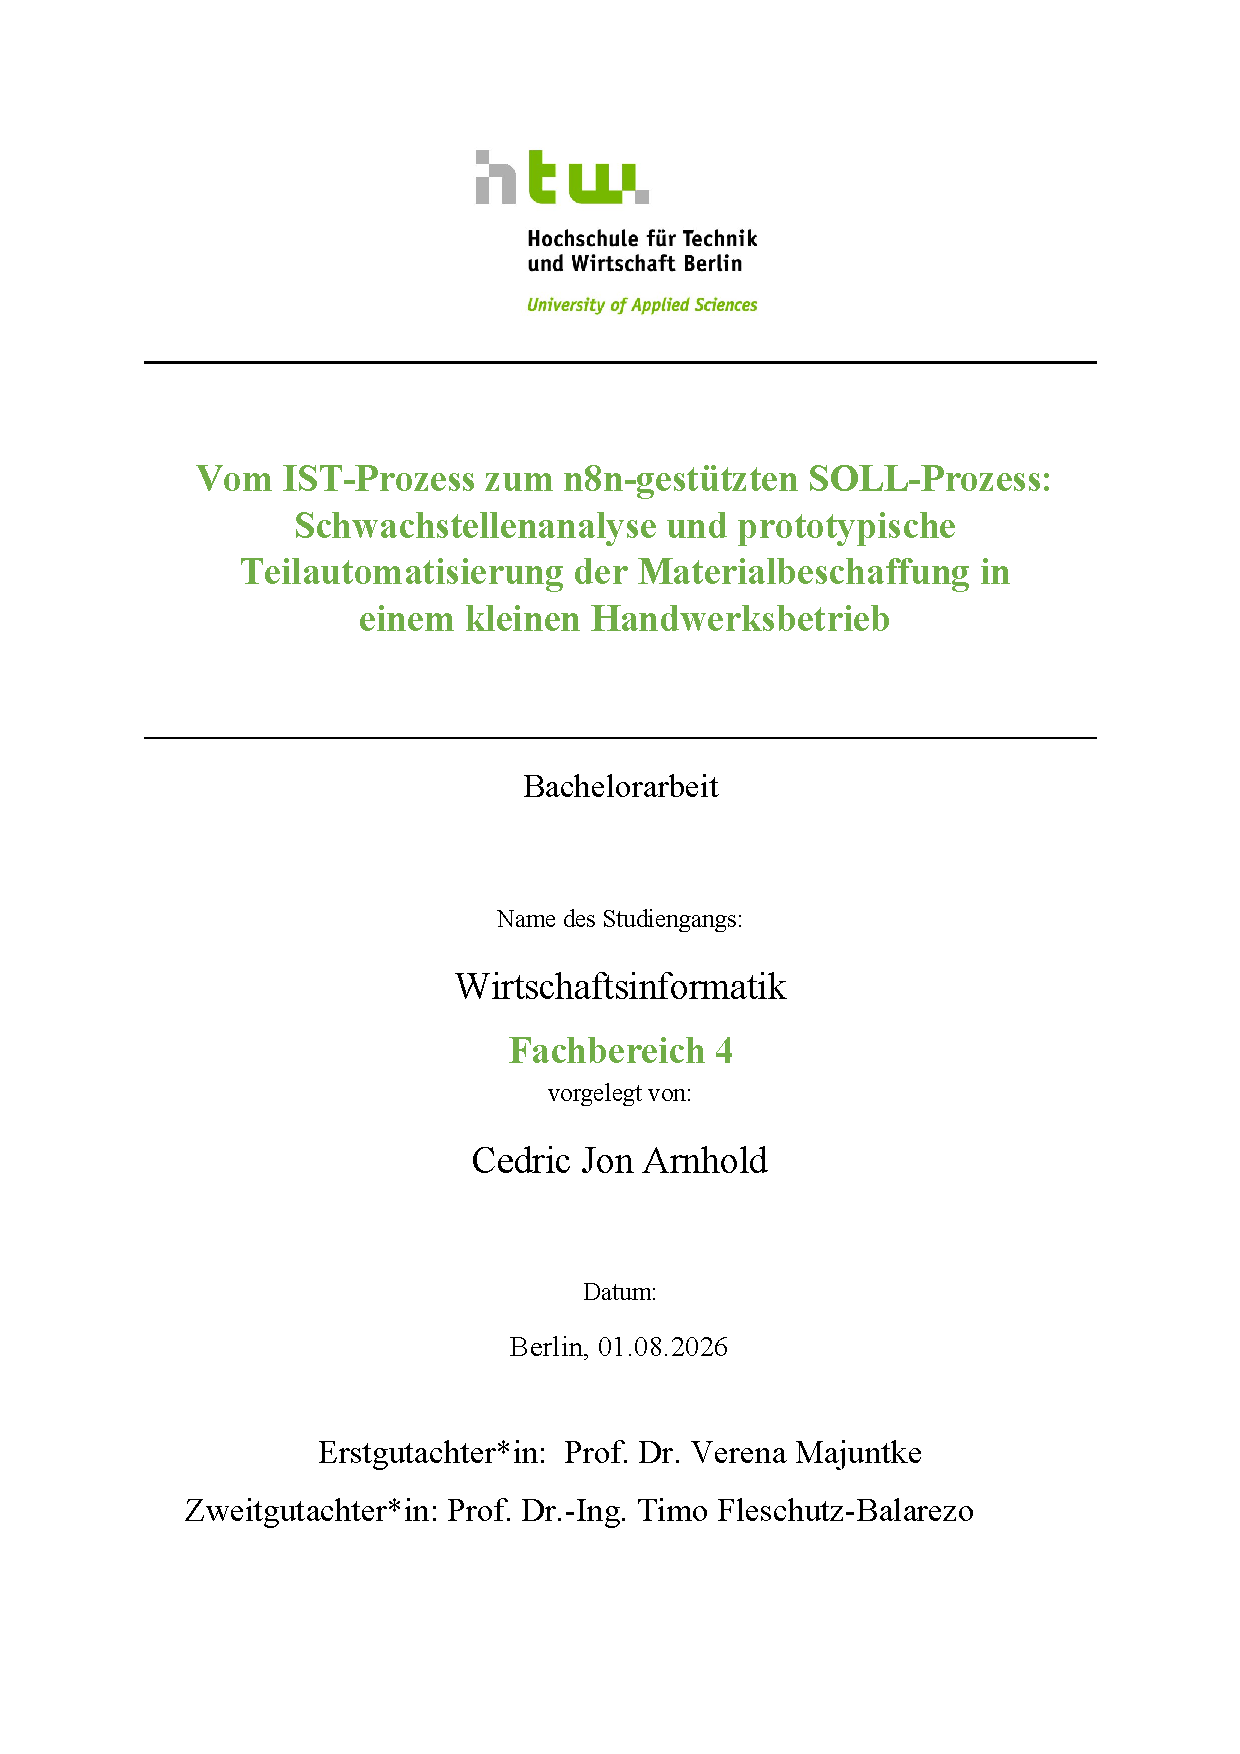
\includepdf[pages=-,pagecommand={\thispagestyle{empty}},fitpaper=true,alt={Deckblatt der Bachelorarbeit mit Titel- und Prüfungsangaben}]{../Deckblattv2.pdf}
\endgroup
\clearpage
\hypersetup{pageanchor=true}

\pagenumbering{roman}

\section*{Abstract (Deutsch)}
\addcontentsline{toc}{frontmatter}{Abstract (Deutsch)}
Diese Bachelorarbeit untersucht, wie der Materialbeschaffungsprozess eines kleinen metallverarbeitenden Handwerksunternehmens systematisch analysiert, mit n8n prototypisch automatisiert und in Handlungsempfehlungen für vergleichbare Kleinst- und Kleinunternehmen überführt werden kann. Ausgangspunkt ist ein manuell geprägter Ablauf, in dem Stücklistenprüfung, Lieferantenzuordnung, Angebotsvergleich, Freigaben, Bestellung und Auftragsbestätigung stark von Erfahrungswissen, E-Mail-Kommunikation und manueller Kontrolle abhängen. Methodisch verbindet die Arbeit einen Design-Science-Ansatz mit einem leitfadengestützten Interview, BPMN-Modellierung, einer an die Fehlermöglichkeits- und -einflussanalyse (FMEA) angelehnten Schwachstellenpriorisierung, einem Anforderungskatalog und fünf fallbasierten Testläufen. Der entwickelte n8n-Prototyp bildet den abgegrenzten Prozessabschnitt von der Stückliste bis zum Abgleich der Auftragsbestätigung ab und nutzt Datei- und E-Mail-Schritte, Code-Nodes, lokale KI-Unterstützung sowie menschliche Kontrollpunkte. Die Evaluation zeigt, dass vollständige Stücklisten verarbeitet, fehlende Normangaben früh gestoppt, fehlende Lieferantenzuordnungen sichtbar gemacht und Zusatzkosten im Angebotsvergleich korrekt berücksichtigt werden können. Unklare Auftragsbestätigungen werden nicht automatisch akzeptiert, sondern in eine menschliche Klärentscheidung überführt. Der Nutzen des Prototyps liegt damit weniger in einer vollständigen Automatisierung der Beschaffung als in der strukturierten Vorbereitung wiederkehrender Prüfschritte, der früheren Sichtbarkeit von Fehlern und der nachvollziehbaren Absicherung externer Entscheidungen. Für einen Produktivbetrieb reichen diese Ergebnisse noch nicht aus. Vergleichbare Unternehmen müssen vor allem Datenqualität, Zuständigkeiten, Mail- und Formularlogik, Wartung, Backup, Monitoring, Datenschutz und klare Freigaberegeln klären, bevor ein solcher Workflow belastbar eingesetzt werden kann.

\clearpage
\section*{Abstract (English)}
\addcontentsline{toc}{frontmatter}{Abstract (English)}
This bachelor’s thesis examines how the material procurement process of a small metalworking enterprise can be systematically analysed, partially automated in a prototype implemented with n8n, and translated into recommendations for comparable micro and small enterprises. The starting point is a largely manual process in which bill of materials verification, supplier assignment, quotation comparison, approvals, ordering, and order confirmation checks depend heavily on experiential knowledge, email communication, and manual oversight. Methodologically, the study combines a design science approach with a guided interview, BPMN modelling, prioritisation based on a simplified \textit{Failure Mode and Effects Analysis} (FMEA), a requirements catalogue, and five case-based test runs. The developed n8n prototype covers the defined process segment from the bill of materials to the verification of the order confirmation and incorporates file- and email-based steps, code nodes, local AI support, and human checkpoints. The evaluation shows that complete bills of materials can be processed, missing standard specifications can be identified at an early stage, missing supplier assignments can be highlighted, and additional costs can be correctly included in quotation comparisons. Unclear order confirmations are not accepted automatically but are referred to a human for clarification. The value of the prototype therefore lies less in fully automating procurement than in structuring recurring checks, identifying errors earlier, and documenting human decisions more transparently. However, these results are not sufficient for production use on their own. Before such a workflow can be deployed reliably, comparable enterprises must clarify requirements concerning data quality, responsibilities, email and form processing, maintenance, backups, monitoring, data protection, and approval rules.

\clearpage
\begingroup
\setlength{\parskip}{0pt}
\tableofcontents
\endgroup
\clearpage

\listoffigures
\addcontentsline{toc}{frontmatter}{Abbildungsverzeichnis}
\clearpage

\listoftables
\addcontentsline{toc}{frontmatter}{Tabellenverzeichnis}
\clearpage

\section*{Abkürzungsverzeichnis}
\addcontentsline{toc}{frontmatter}{Abkürzungsverzeichnis}
\begingroup
\renewcommand{\arraystretch}{0.88}
\begin{tabularx}{\textwidth}{@{}p{2.2cm}X@{}}
    AB & Auftragsbestätigung \\
    AF & Fachliche Anforderung im SOLL-Prozess \\
    API & Application Programming Interface, Programmierschnittstelle \\
    ASTM & ASTM International \\
    BPA & Business Process Automation \\
    BPM & Business Process Management \\
    BPMN & Business Process Model and Notation \\
    CLI & Command Line Interface \\
    CSV & Comma-Separated Values \\
    DIN & Deutsches Institut für Normung \\
    DSGVO & Datenschutz-Grundverordnung \\
    EN & Europäische Norm \\
    ERP & Enterprise Resource Planning \\
    FMEA & Failure Mode and Effects Analysis \\
    HTTP & Hypertext Transfer Protocol \\
    ID & Identifikator \\
    IMAP & Internet Message Access Protocol \\
    IT & Informationstechnik \\
    JSON & JavaScript Object Notation \\
    KI & Künstliche Intelligenz \\
    KKU & Kleinst- und Kleinunternehmen \\
    KMU & Kleine und mittlere Unternehmen \\
    KP & Kontrollpunkt \\
    KPI & Key Performance Indicator \\
    LAN & Local Area Network \\
    LLM & Large Language Model \\
    NF & Nicht-funktionale Anforderung \\
    NoOp & No Operation, Knoten ohne inhaltliche Verarbeitung \\
    OAuth & Open Authorization \\
    OECD & Organisation for Economic Co-operation and Development \\
    PID & Process Identifier, Prozesskennung \\
    REST & Representational State Transfer \\
    RPA & Robotic Process Automation \\
    RPZ & Risikoprioritätszahl \\
    SaaS & Software as a Service \\
    SMTP & Simple Mail Transfer Protocol \\
    TF & Testfall \\
    URL & Uniform Resource Locator \\
    UTF-8 & 8-bit Unicode Transformation Format \\
\end{tabularx}
\endgroup

\clearpage
\section*{KI-Verzeichnis}
\addcontentsline{toc}{frontmatter}{KI-Verzeichnis}
Im Folgenden wird transparent dokumentiert, welche KI-Tools im Rahmen dieser Bachelorarbeit eingesetzt und wofür diese verwendet wurden.

\begingroup
\renewcommand{\baselinestretch}{1.0}\selectfont
\renewcommand{\arraystretch}{0.9}
\setlength{\tabcolsep}{3pt}
\begin{tabularx}{\textwidth}{
    @{}
    >{\raggedright\arraybackslash}p{0.14\textwidth}
    >{\raggedright\arraybackslash}p{0.18\textwidth}
    >{\raggedright\arraybackslash}p{0.22\textwidth}
    >{\raggedright\arraybackslash}X
    @{}
}\toprule
    Tool & Modell/Dienst & Betroffene Teile & Verwendungszweck \\
    \midrule
    noScribe & faster-whisper-large-v3 (OpenAI) & Interviewtranskript und Anhang A1 & Automatische Ersttranskription, anschließend eigenständige Prüfung und Korrektur anhand der Audioaufnahme. \\        
    \midrule
    Google Scholar & Suchdienst & Literaturrecherche, übergreifend & Recherche nach wissenschaftlicher Literatur, Auswahl, Bewertung und Zitierung erfolgten eigenständig. \\
    \midrule
    ChatGPT & 5.2 Thinking & Literaturrecherche und Strukturierung, übergreifend & Unterstützung bei Suchbegriffen, Quellenüberblick und Gliederungsoptionen. Quellen und Aussagen wurden eigenständig geprüft. \\
    \midrule
    Claude Code & Opus 4.7 & n8n-Implementierung und Testnachweise & Unterstützung bei Prompt- und Codeanpassungen, Fehlersuche und Testdokumentation. Bewertung und finale Anpassungen erfolgten eigenständig. \\
    \midrule
    ChatGPT & 5.5 & Abstract (Deutsch) & Unterstützung bei der sprachlichen Optimierung und Strukturierung des deutsch formulierten Abstracts. Eigenständige fachliche und sprachliche Prüfung. \\
    \midrule
    DeepL & Übersetzung & Abstract (English) & Übersetzung des deutsch formulierten Abstracts, eigenständige fachliche und sprachliche Prüfung. \\
    \midrule
    ChatGPT & 5.6 Sol & 1.2 (S. 2 ff.)\newline 2.3 (S. 6 ff.)\newline 3.4 (S. 14 ff.)\newline 3.5 (S. 16 ff.)\newline 4.2 (S. 22 ff.)\newline 4.4 (S. 25 ff.)\newline 5.2 (S. 32 ff.) \newline 6.2 (S. 41 ff.) \newline 8.1 (S. 54 ff.) \newline 8.2 (S. 55 ff.) & Unterstützung bei der sprachlichen Optimierung und Strukturierung einzelner Abschnitte \\
    \midrule
    Codex & GPT-5 & Schlussredaktion und Qualitätssicherung & Unterstützung bei LaTeX-Korrekturen, Build- und PDF-Prüfung. \\
\bottomrule
\end{tabularx}
\endgroup

\clearpage
\pagenumbering{arabic}

% --- Hauptteil ---
\section{Einleitung}

\subsection{Motivation und Relevanz}
Kleine Handwerksbetriebe müssen Digitalisierungsvorhaben häufig mit knappen Ressourcen in das operative Tagesgeschäft und in altbewährte Strukturen einbinden \parencite{beuchel_digitalisierung_2024}. Im betrachteten Metallbaubetrieb müssen aus einer fachlich erstellten Stückliste passende Materialien, Bezugsquellen, Preise, Lieferzeiten und Bestellfreigaben abgeleitet werden. Diese Arbeitsschritte hängen bisher stark von Erfahrungswissen, E-Mail-Kommunikation und manueller Kontrolle ab. Der Prozess funktioniert im Tagesgeschäft, wird bei parallelen Aufträgen allerdings zeitaufwendig und fehleranfällig.

Business Process Automation (BPA) kann die für Routinetätigkeiten benötigte Zeit verringern und Beschäftigte von manuellem Aufwand entlasten \parencite{moreira_business_2024}. Für Kleinst- und Kleinunternehmen (KKU) ist dies besonders relevant, da begrenzte Budgets, geringe personelle Ressourcen und fehlende digitale Kompetenzen die Auswahl und Einführung geeigneter Lösungen erschweren \parencite{moreira_business_2024}. Im Handwerk zeigt sich diese Spannung deutlich. Im Jahr 2022 lag der Anteil der Handwerksbetriebe, die die digitale Transformation als Chance wahrnahmen, bei 77\,\%, während lediglich 8\,\% sie als risikobehaftet wahrnahmen \parencite{beuchel_digitalisierung_2024}. \Textcite{beuchel_digitalisierung_2024} beschreiben zugleich knappe Personalressourcen, Unsicherheit, Kosten und geringe Digitalisierungsaffinität als zentrale Herausforderungen, insbesondere bei Kleinstbetrieben mit weniger als zehn Beschäftigten. Dies ist im Tagesgeschäft anspruchsvoll, weil Beschaffung, Kundenabstimmung und Fertigung häufig parallel laufen.

Die Arbeit knüpft an dieses Praxisproblem an und untersucht, wie sich der Materialbeschaffungsprozess eines kleinen Handwerksunternehmens systematisch analysieren, mit n8n prototypisch automatisieren und in Handlungsempfehlungen für vergleichbare Unternehmen überführen lässt. Dabei wird n8n als knotenbasierte Workflow-Plattform betrachtet. Nodes können einen Ablauf starten, Daten verarbeiten oder Ergebnisse weitergeben \parencite{n8n_docs_2026}. Self-Hosting ist unter anderem über npm oder Docker möglich \parencite{n8n_docs_2026}. Im untersuchten Materialbeschaffungsprozess treten Stücklistenprüfung, Lieferantenzuordnung, Angebotsvergleich, Freigaben und Auftragsbestätigungsprüfung wiederholt auf. Diese fallbezogene Abfolge bildet den Ausgangspunkt der prototypischen Automatisierung.

\subsection{Stand der Forschung}
Eine systematische Literaturübersicht weist insbesondere auf eine mögliche Lücke bei Modellen hin, die den gesamten Weg einer BPA-Einführung in KMU anleiten \parencite{moreira_business_2024}. Die darauf aufbauende Methodik verbindet Prozessauswahl und -gestaltung mit Implementierung und anschließender Steuerung der Lösung \parencite{moreira_methodology_2025}. Der RPA-spezifische Bewertungsrahmen von \textcite{wellmann_framework_2020} prüft anhand eines Kriterienrasters, ob eine einzelne Prozessaktivität vor der Umsetzung für RPA geeignet ist. Er bündelt dreizehn Kriterien in fünf Perspektiven und betrachtet unter anderem Regelbasiertheit, Prozessreife, Datenstruktur, Fehlerquote, Häufigkeit und Dauer. Die Eignungsprüfung setzt außerdem voraus, dass ein verbesserungsbedürftiger Prozess nicht unverändert automatisiert wird \parencite{stravinskiene_process_2021}. Zusammengenommen wird für die vorliegende Arbeit daraus ein Vorgehen abgeleitet, das von der begründeten Prozessauswahl über die fachliche Vorbereitung bis zur geregelten Umsetzung reicht. Die RPA-bezogenen Eignungskriterien dienen dabei als Orientierung für die Auswahl und Vorbereitung workflowbasierter Prozessschritte mit n8n.

Eine positive Eignungsbewertung garantiert allerdings noch keinen tragfähigen Betrieb. \Textcite{herm_framework_2023} ordnen Support und Wartung als fortlaufende Aufgaben ein, die nach einer ersten Erprobungsphase bestehen bleiben, und fordern bereits zu Projektbeginn die Klärung von Rollen. Aus den zuvor beschriebenen Rahmenbedingungen wird für kleine Handwerksbetriebe abgeleitet, dass Ressourcenengpässe diese organisatorische Aufgabe zusätzlich erschweren. Damit werden Prozessauswahl, Prozessverbesserung und Betriebsorganisation im untersuchten Fall als zusammengehörige Voraussetzungen behandelt.

Auf den Beschaffungskontext übertragen zeigt sich eine klare Grenze der Automatisierung. Wiederkehrende operative Aufgaben bieten Entlastungspotenzial, das durch uneinheitliche Daten, Lieferantenschnittstellen und fehlende organisatorische Reife begrenzt wird \parencite{flechsig_robotic_2022}. Menschliche Vorbereitung und Aufsicht wurden bei automatisierten Einkaufsschritten zumindest teilweise beobachtet \parencite{viale_impact_2020}. Strategische Verhandlungen sowie ethische und kontextabhängige Entscheidungen benötigen weiterhin menschliche Aufsicht \parencite{santos_rebooting_2025}. Auf den untersuchten Prozess übertragen ergibt sich daraus eine Teilautomatisierung, die Daten vorbereitet und prüft, Entscheidungen mit Außenwirkung aber an nachvollziehbare Freigaben bindet.

Die in dieser Arbeit herangezogene n8n-spezifische Literatur bleibt auf einzelne Anwendungsszenarien begrenzt. \Textcite{venkiteela_n8n_2025} betrachtet n8n als Plattform für Workflow-Integration und KI-Orchestrierung. \Textcite{amir_evaluating_2026} untersuchen in einem Preprint einen kleinen Workflow zur Verarbeitung von Leads mit begrenzter Datenbasis und fordern für weitergehende Aussagen größere Datensätze sowie Vergleiche mehrerer Low-Code-Plattformen. Diese Beiträge liefern noch kein durchgängiges Vorgehen von der IST-Analyse über prüfbare Anforderungen bis zu einer getesteten Umsetzung und betrieblichen Handlungsempfehlungen. An dieser Forschungslücke setzt die vorliegende Fallstudie an.

\subsection{Zielsetzung und Abgrenzung}
\label{sec:zielsetzung-abgrenzung}
Ziel dieser Arbeit ist es, den gegenwärtig manuell geprägten Materialbeschaffungsprozess in einem kleinen metallverarbeitenden Handwerksunternehmen mit weniger als zehn Mitarbeitenden zu analysieren und daraus einen automatisierten SOLL-Prozess abzuleiten. Dieser SOLL-Prozess wird mit n8n prototypisch umgesetzt und anhand definierter Testfälle geprüft. Die Ergebnisse sollen zeigen, welche Prozessteile technisch abbildbar sind, welche Schwachstellen durch Automatisierung reduziert werden können und welche Voraussetzungen vergleichbare KKU beachten müssen.

Die Arbeit ist ausdrücklich als Prototypen- und Fallstudienarbeit abgegrenzt. Untersucht wird der Prozess von der materialbezogenen Bedarfsermittlung auf Basis einer Stückliste bis zum Abgleich der Auftragsbestätigung und zur Übergabe an den manuellen Wareneingang. Nicht untersucht werden ein produktiver Dauerbetrieb, eine vollständige Einbindung realer Lieferantensysteme, eine Langzeitmessung nach dem Rollout oder eine vollständige betriebswirtschaftliche Amortisationsrechnung. Externe Warteereignisse, echte Lieferantenkommunikation und produktive Bestellungen werden dort simuliert, wo dies für einen verantwortbaren Prototyp notwendig ist. Die Handlungsempfehlungen beziehen sich daher auf Voraussetzungen, Risiken und Übertragbarkeit, nicht auf eine unmittelbar produktionsreife Einführung.

\subsection{Forschungsfragen und Aufbau}
Aus der Zielsetzung ergibt sich folgende leitende Forschungsfrage. \enquote{Wie kann der Materialbeschaffungsprozess eines kleinen Handwerksunternehmens systematisch analysiert, prototypisch mit n8n automatisiert und in Handlungsempfehlungen für vergleichbare Kleinst- und Kleinunternehmen überführt werden?}

Die leitende Forschungsfrage wird mithilfe von vier Teilfragen beantwortet.:

\begin{enumerate}
    \item Welche Schwachstellen weist der bestehende Materialbeschaffungsprozess auf?
    \item Welche Anforderungen ergeben sich daraus an einen automatisierten SOLL-Prozess?
    \item In welchem Umfang lässt sich dieser SOLL-Prozess mit n8n prototypisch umsetzen und testen?
    \item Welche technischen, organisatorischen, wirtschaftlichen und datenschutzbezogenen Risiken müssen ähnliche Unternehmen beachten?
\end{enumerate}

Der Aufbau folgt der Forschungslogik von der Analyse bis zur Bewertung. Zunächst werden der Design-Science-Ansatz, die Erhebung des IST-Prozesses über ein leitfadengestütztes Interview und die Verbindung von Schwachstellen, Anforderungen, Testfällen und Handlungsempfehlungen begründet. Anschließend werden die theoretischen Grundlagen zu BPA, Low-Code- und Workflow-Systemen, n8n sowie relevanten Betriebs- und Bewertungskriterien eingeordnet. Darauf aufbauend werden der Praxisfall analysiert, der betrachtete Beschaffungsprozess abgegrenzt und Anforderungen an den SOLL-Prozess abgeleitet. Danach folgen SOLL-Modell, Anforderungskatalog, n8n-Lösungsarchitektur, prototypische Umsetzung und Tests. Abschließend werden die Ergebnisse bewertet, die Forschungsfragen beantwortet und Handlungshinweise für vergleichbare Kleinst- und Kleinunternehmen abgeleitet.

\clearpage
\section{Methodik}
Die methodische Grundlage muss den Weg vom Interview bis zum Prototyp nachvollziehbar machen. Dafür werden Design Science, qualitative Prozesserhebung, Modellierung mit der \textit{Business Process Model and Notation} (BPMN), Schwachstellenpriorisierung und testbasierte Bewertung zu einer gemeinsamen Untersuchungslogik verbunden.

\subsection{Design-Science-Ansatz}
Methodisch folgt die Arbeit dem Design-Science-Ansatz, da ein praxisnahes Artefakt entwickelt und bewertet wird. \Textcite{peffers_design_2007} gliedern den Design-Science-Prozess unter anderem in Gestaltung und Entwicklung, Demonstration und Evaluation. Das Artefakt umfasst den technischen n8n-Prototyp zusammen mit dem analysierten IST-Prozess, dem abgeleiteten SOLL-Modell, dem Anforderungskatalog, der prototypischen Umsetzung, den Testfällen und den daraus abgeleiteten Handlungsempfehlungen.

Das Vorgehen beginnt mit einer strukturierten Literaturrecherche zu Prozessautomatisierung, Automatisierungseignung und Rahmenbedingungen kleiner Unternehmen. Die Literatur liefert die theoretischen und methodischen Grundlagen für die Untersuchung. Für die methodische Abfolge wird der BPA-Ansatz von \textcite{moreira_methodology_2025} herangezogen. Die Kriterienraster von \textcite{wellmann_framework_2020} und \textcite{choi_candidate_2021} unterstützen die Beurteilung der Automatisierungseignung. Die Einordnung und Bewertung des konkreten Praxisfalls erfolgt dagegen auf Grundlage der eigenen empirischen Untersuchung. Hersteller-, Tool- und Webquellen werden ergänzend genutzt, wenn technische Eigenschaften, Versionen oder Abrechnungslogiken beschrieben werden. Methodische und bewertende Aussagen stützen sich dagegen auf wissenschaftliche Literatur. Anschließend wird der bestehende Materialbeschaffungsprozess empirisch über ein leitfadengestütztes Interview erhoben. Die strukturierte Prozessaufnahme und die anschließende Schwachstellenanalyse orientieren sich ergänzend an der Prozessoptimierungsliteratur \parencite{kompetenzzentrum_augsburg_prozessoptimierung_2020}. Für die Darstellung des IST-Prozesses wird BPMN als standardisierte grafische Prozessnotation verwendet \parencite{object_management_group_bpmn_2014}. Auf dieser Grundlage werden Anforderungen an den SOLL-Prozess formuliert und mit n8n prototypisch umgesetzt. Die Bewertung nutzt die Testfälle TF1 bis TF5 aus Anhang~\ref{anhang:testprotokolle} sowie technische, organisatorische, wirtschaftliche und datenschutzbezogene Kriterien.

Die Methode ist bewusst fallbezogen angelegt. Sie liefert keine allgemeingültige Produktauswahl, sondern zeigt, wie ein kleiner Handwerksbetrieb seinen Beschaffungsprozess nachvollziehbar analysiert, eine realistische n8n-Automatisierung erprobt und daraus übertragbare Handlungshinweise ableitet. Das funktioniert nur, wenn Prozesswissen, Datenqualität und Verantwortlichkeiten nicht als Nebenthemen behandelt werden.

\subsection{Erhebung des IST-Prozesses durch leitfadengestütztes Interview}
Der bestehende Materialbeschaffungsprozess wird mithilfe eines leitfadengestützten Interviews erhoben. Die Konzeption und Durchführung des Interviews orientieren sich an \textcite{helfferich_leitfaden_2022}. Als fachkundige Interviewperson wird die Person einbezogen, die den Prozess im Unternehmen ausführt oder verantwortet. Aufgrund ihrer unmittelbaren Prozesserfahrung kann sie Auskunft über Arbeitsschritte, Entscheidungswege, verwendete Dokumente und Systeme sowie über Ausnahmen und typische Fehlerquellen geben. Die im Interview gewonnenen Informationen bilden eine eigene empirische Datengrundlage der Arbeit. Das Interview wird daher als Primärdatenerhebung dokumentiert und nicht als Literaturquelle behandelt.

Der Interviewleitfaden ist für den vorliegenden Fall prozessorientiert aufgebaut. Er erfasst zunächst den Auslöser des Beschaffungsprozesses, die verwendeten Eingabedaten wie Stücklisten oder Materialangaben und die beteiligten Rollen. Danach werden einzelne Aktivitäten, genutzte Systeme, manuelle Übertragungen, Kommunikationswege, Wartezeiten, Kontrollschritte und Ausnahmefälle abgefragt. Dadurch wird erkennbar, ob die Aussagen ein tragfähiges IST-Modell statt einer allgemeinen Beschaffungsbeschreibung ermöglichen. Die dokumentierte Interviewfassung belegt die Themen Rolle und Materialbestellung, Prozessablauf, Stückliste, Lieferantenauswahl, Kommunikation, Wartezeiten sowie Fehler- und Kontrollpunkte (vgl. \hyperref[anhang:interviewleitfaden]{Anhang~\ref*{anhang:interviewleitfaden}}, Zeitmarken \hyperlink{itv:rolle-materialbestellung}{00:01:34--00:02:52}, \hyperlink{itv:prozess-stueckliste}{00:03:25--00:05:21}, \hyperlink{itv:lieferanten-angebote}{00:07:07--00:18:05}, \hyperlink{itv:kommunikation-fehler}{00:24:14--00:32:49} und \hyperlink{itv:kontrolle-freigabe}{00:43:58--00:45:33}). Anhang~\ref{anhang:interviewleitfaden} dokumentiert die für die Auswertung verwendete Interviewfassung.

Die automatische Ersttranskription erfolgte mit noScribe in Version 0.6 \parencite{droege_noscribe_2026}. Anschließend wurde das Transkript anhand der Audioaufnahme geprüft und korrigiert.

\subsection{Schwachstellenanalyse, Anforderungen und Evaluation}
\label{sec:evaluationslogik}
Aus dem Interview werden die relevanten Aktivitäten, Rollen, Dokumente, Systeme, Entscheidungen und Ausnahmen herausgearbeitet und in ein BPMN-basiertes IST-Modell überführt. BPMN dient dabei als standardisierte grafische Prozessnotation \parencite{object_management_group_bpmn_2014}. Die Prozessanalyse und -gestaltung gehen der technischen Umsetzung voraus \parencite{moreira_methodology_2025}. Das IST-Modell bildet den aktuellen Ablauf ab und wird genutzt, um Medienbrüche, manuelle Übertragungen, Wartezeiten, unklare Verantwortlichkeiten, fehlende Datenstrukturen und fehleranfällige Kontrollpunkte zu identifizieren.

Die identifizierten Schwachstellen werden anschließend eingeordnet und priorisiert. Das Vorgehen orientiert sich an Ansätzen der Prozessoptimierung \parencite{kompetenzzentrum_augsburg_prozessoptimierung_2020}. Entscheidend ist dabei nicht allein, ob ein Schritt technisch automatisierbar ist, sondern ob seine Automatisierung fachlich sinnvoll und für ein kleines Unternehmen beherrschbar ist. In Anlehnung an \textcite{wellmann_framework_2020} werden insbesondere Häufigkeit, Zeitwirkung, Fehlerrisiko, Regelbasiertheit und Datenqualität berücksichtigt. Für den untersuchten Fall wird der Kriterienrahmen um die Abhängigkeit von externen Beteiligten und den organisatorischen Aufwand erweitert. Diese Ergänzung berücksichtigt, dass Lieferanten- und Kundenreaktionen außerhalb des unmittelbaren Einflussbereichs des Unternehmens liegen und die Umsetzbarkeit von den verfügbaren personellen und technischen Ressourcen abhängt.

Die priorisierten Schwachstellen bilden den Ausgangspunkt für das SOLL-Modell. Es unterscheidet zwischen automatisierten Schritten, systemgestützter Unterstützung und bewusst beibehaltenen manuellen Freigaben. Aus diesem Modell wird der Anforderungskatalog für den n8n-Prototyp abgeleitet. Die Anforderungen beschreiben erwartete Eingaben, Verarbeitungsschritte und Ausgaben. Wo es erforderlich ist, legen sie außerdem Freigaben oder Fehlermeldungen fest. Dadurch bleibt nachvollziehbar, wie Interview, IST-Modell, Schwachstellenpriorisierung, SOLL-Modell und technische Umsetzung aufeinander aufbauen.

Fünf risikobasiert ausgewählte \textit{Testfälle} (TF1 bis TF5) prüfen die abgeleiteten Anforderungen am Prototyp. Für jeden Testfall werden Prüfziel, Eingabe, erwartetes und tatsächliches Ergebnis, Ausführungsnachweis, Abweichungen, Fehlerbehandlung sowie der Bezug zu Anforderungen und Kontrollpunkten dokumentiert. Da die Testfälle keinen vollständigen Abnahmetest ersetzen, bleibt die Bewertung auf das jeweils festgelegte Prüfziel und den dokumentierten Pfad beschränkt. Beobachtungen außerhalb dieses Umfangs werden getrennt als Grenzen des Prototyps ausgewiesen.

Abschließend werden Testergebnisse, Anforderungen und priorisierte Schwachstellen zusammengeführt. Die daraus abgeleiteten Handlungsempfehlungen für vergleichbare KKU sind eine eigene Synthese aus Fallanalyse, Artefakt, Testbefunden und Literatur. Sie betreffen Prozessreife, Datenqualität, Verantwortlichkeiten, Betriebsmodell, Kosten, Datenschutz, Sicherung, Aktualisierungen und interne Kompetenzen.

\clearpage
\section{Theoretische Grundlagen}
Die theoretischen Grundlagen liefern den Kriterienrahmen für die Prozessautomatisierung im Praxisfall. Im Mittelpunkt stehen Wiederholbarkeit, Regelbasiertheit, Datenqualität, Ausnahmebehandlung und menschliche Kontrollpunkte. Für die spätere Evaluation kommen funktionale Abdeckung, Kostenberechnung, Protokollierbarkeit, Wartbarkeit, Integration, Datenschutz, betrieblicher Aufwand und Betriebsfähigkeit hinzu. Damit richtet sich der Blick auf automatisierbare Prozessanteile und die Grenzen, die im Betrieb bestehen bleiben.

\subsection{Workflow-Systeme und Low-Code-Plattformen}
\textit{Business Process Management} (BPM) beschreibt die systematische Gestaltung, Analyse, Ausführung, Überwachung und Verbesserung von Geschäftsprozessen. Es versteht Abläufe als Zusammenspiel aus Aktivitäten, Rollen, Daten, Systemen und organisatorischen Zielen. BPA setzt auf dieser prozessorientierten Grundlage auf und überführt geeignete Prozessschritte in regel- oder systemgestützte Abläufe. Ziel ist es, wiederkehrende Routinetätigkeiten zu reduzieren, Durchlaufzeiten zu verkürzen, die Genauigkeit zu erhöhen und Beschäftigte von manuellen Aufgaben zu entlasten \parencite{moreira_business_2024}. Für kleine Unternehmen ist dieser Nutzen besonders relevant, weil operative Engpässe häufig dort entstehen, wo fachliche Arbeit, Verwaltung und Kommunikation parallel bewältigt werden müssen.

Workflow-Systeme bilden die technische Ausführungsschicht für definierte Prozesslogik. Sie verbinden auslösende Ereignisse, Verarbeitungsschritte, Datenflüsse, Bedingungen, Integrationen und Statusübergänge zu nachvollziehbaren Abläufen \parencite{moreira_business_2024}. In der Literatur werden Workflow-Management-Systeme beziehungsweise Business-Process-Management-Systeme neben Robotic Process Automation (RPA), Enterprise Resource Planning (ERP) und Künstlicher Intelligenz (KI) als zentrale Werkzeuggruppen der BPA eingeordnet \parencite{moreira_business_2024}. Für den hier betrachteten n8n-Prototyp ist diese Einordnung wichtig, da nicht primär eine bestehende Benutzeroberfläche nachgeahmt wird. Stattdessen werden Ereignisse, Daten, E-Mails, Regeln, Freigaben und Schnittstellen in einem Workflow koordiniert \parencite{n8n_docs_2026,venkiteela_n8n_2025}.

Low-Code- und No-Code-Plattformen ergänzen diese Entwicklung, indem sie Anwendungs- und Prozesslogik über visuelle oder deklarative Mittel zugänglich machen. No-Code zielt auf Konfiguration ohne eigene Programmierung, während Low-Code visuelle Modellierung mit punktuellen Code-Erweiterungen kombiniert \parencite{abendroth_werkzeug_2024}. Modularität und Wiederverwendung vorhandener Komponenten können die Entwicklungseffizienz steigern und die Wartbarkeit erleichtern \parencite{abendroth_werkzeug_2024}. Verwaltung, Sicherheit, Skalierbarkeit und Schulung bleiben zugleich Anforderungen an Low-Code- und No-Code-Einsätze \parencite{ozman_systematic_2025}. n8n lässt sich in diesem Zusammenhang als Low-Code-orientierte Workflow- und Integrationsplattform einordnen. Workflows werden aus miteinander verbundenen Nodes aufgebaut \parencite{n8n_docs_2026}. Der Code-Node ermöglicht die Ergänzung eigener Logik in JavaScript oder Python, während der HTTP-Request-Node REST-Schnittstellen in den Workflow einbindet \parencite{n8n_docs_2026}. 

Von Workflow-Automation und BPA ist die Robotic Process Automation (RPA) begrifflich abzugrenzen. \textcite{van_der_aalst_robotic_2018} beschreiben RPA als eine Form der Automatisierung, bei der Software über die Benutzeroberflächen bestehender Anwendungssysteme ähnlich wie ein Mensch interagiert. Die eingesetzten Software-Bots bearbeiten typischerweise strukturierte, regelbasierte und repetitive Aufgaben \parencite{syed_robotic_2020}. Dieser nicht-invasive Ansatz kann insbesondere dann relevant sein, wenn bestehende Anwendungssysteme keine geeigneten Schnittstellen bereitstellen \parencite{syed_robotic_2020}.

BPA nimmt demgegenüber eine breitere Prozessperspektive ein. Die von \textcite{moreira_business_2024} betrachteten BPA-Ansätze berücksichtigen neben der technischen Umsetzung unter anderem Prozessanalyse, Technologiewahl, Monitoring, Rollen und organisatorische Veränderungen. Für diese Arbeit wird RPA daher als Möglichkeit zur Automatisierung einzelner menschlicher Systeminteraktionen eingeordnet, während BPA die Auswahl, Gestaltung, Umsetzung und organisatorische Einbettung automatisierter Prozessanteile umfasst. BPM bildet den übergeordneten Ansatz zur Analyse und Gestaltung von Geschäftsprozessen. Workflow-Systeme übernehmen die technische Steuerung der daraus abgeleiteten Abläufe.

Der Materialbeschaffungsprozess eines kleinen Handwerksunternehmens enthält wiederkehrende Prüf-, Zuordnungs-, Kommunikations- und Freigabeschritte. Dazu gehören die Prüfung von Stücklistendaten, die Zuordnung geeigneter Bezugsquellen, die Vorbereitung von Anfragen, der Angebotsvergleich, die Bestellfreigabe und die spätere Kontrolle von Abweichungen. Studien zur Automatisierung in der Materialbeschaffung zeigen, dass digitale Prozessautomatisierung operative Beschaffungsaufgaben entlasten und Effizienz, Qualität sowie Durchlaufzeiten verbessern kann, sofern Prozessreife, Datenstruktur und organisatorische Einbindung berücksichtigt werden \parencite{flechsig_robotic_2022,santos_rebooting_2025,viale_impact_2020}. Der Prototyp ist daher als workflowbasierte BPA zu verstehen. Er soll wiederkehrende und regelbasierte Prozessanteile unterstützen, ohne fachliche Entscheidungen und wirtschaftlich wirksame Freigaben vollständig zu ersetzen.

\subsection{Kriterien für automatisierungsgeeignete Prozesse}
Die Beurteilung der Automatisierungseignung setzt ein belastbares Prozessverständnis voraus. Ein Prozess sollte nicht erst im Automatisierungswerkzeug sichtbar werden, sondern zuvor fachlich beschrieben, abgegrenzt und modelliert sein. Für diese Arbeit bildet BPMN die Modellierungsgrundlage, weil die Notation Geschäftsprozesse über Ereignisse, Aktivitäten, Gateways und Sequenzflüsse strukturiert darstellt und Rollen oder beteiligte Organisationseinheiten über Pools und Lanes sichtbar machen kann \parencite{object_management_group_bpmn_2014}. Dadurch lassen sich Arbeitsschritte, Entscheidungen, Rücksprünge und Verantwortlichkeiten so dokumentieren, dass fachliche und technische Betrachtung miteinander verbunden werden können. Gerade in kleinen Unternehmen ist diese gemeinsame Sicht wichtig, weil Prozesswissen häufig an einzelne Personen gebunden ist und nicht vollständig in Systemen oder Prozesshandbüchern vorliegt \parencite{beuchel_digitalisierung_2024,moreira_methodology_2025}.

Für die Automatisierung erfüllt das BPMN-Modell zwei Aufgaben. Es bildet den fachlichen Ablauf ab und zeigt zugleich, wo Regeln greifen, Daten übertragen werden, Wartezeiten entstehen oder Zuständigkeiten nicht eindeutig sind. \Textcite{moreira_methodology_2025} ordnen die BPMN-Modellierung und die Festlegung von \textit{Key Performance Indicators} (KPI) dem Prozessdesign zu, das der technischen Umsetzung vorausgeht. \Textcite{stravinskiene_process_2021} zeigen zudem, dass ausbleibende Prozessoptimierung zu ineffizienter Administration bis hin zur Reproduktion der Fehlerquellen führen und somit die erwarteten Ergebnisse einer RPA-Einführung verfehlen kann. Im vorliegenden Praxisfall wird daher zunächst der Weg von der Bedarfsermittlung über Prüfung, Lieferantenzuordnung und Angebotsvergleich bis zu den Freigaben modelliert. Erst danach werden die fachlichen Schritte in n8n-Nodes übersetzt.

Ein zentrales Kriterium automatisierungsgeeigneter Prozesse ist Wiederholbarkeit. Automatisierung lohnt sich vor allem bei Tätigkeiten, die regelmäßig auftreten und nach ähnlichen Mustern ablaufen. In der Literatur werden automatisierbare Prozesse häufig als repetitiv, regelbasiert, standardisiert, reif und möglichst wenig komplex beschrieben \parencite{moreira_business_2024}. Das RPA-spezifische Eignungs-Framework von \textcite{wellmann_framework_2020} konkretisiert dies über Standardisierung, Prozessreife, Determinismus, Häufigkeit, Dauer, Datenstruktur und Fehleranfälligkeit. \Textcite{choi_candidate_2021} betonen zusätzlich Frequenz, Periodizität und Dauer als Auswahlmerkmale. Ein einmaliger oder stark situativer Vorgang ist daher weniger geeignet als ein wiederkehrender Arbeitsschritt mit eindeutigen Prozesselementen, stabiler Ausführungsreihenfolge und regelbasierten Entscheidungen.

Neben der Häufigkeit ist die Regelbasiertheit entscheidend. Ein Prozessschritt ist besonders gut automatisierbar, wenn klar ist, welche Bedingungen geprüft werden, welche Daten dafür erforderlich sind und welches Ergebnis daraus folgt. Im Materialbeschaffungsprozess betrifft dies beispielsweise die Prüfung, ob Pflichtfelder einer Stücklistenposition vorhanden sind, ob eine Norm angegeben wurde, ob eine passende Lieferantenkategorie existiert oder ob ein Gesamtpreis aus Stückpreis und Zusatzkosten korrekt berechnet werden kann. Tätigkeiten, die stark von Verhandlung, situativem Erfahrungswissen oder wirtschaftlicher Abwägung abhängen, sollten dagegen nicht vollständig automatisiert werden. Die Literatur zur Beschaffungsautomatisierung weist darauf hin, dass menschliches Urteilsvermögen in Verhandlungen, ethischen Abwägungen oder fachlich sensiblen Entscheidungen weiterhin erforderlich bleibt \parencite{santos_rebooting_2025}.

Datenqualität ist ein weiteres Kernkriterium. Im RPA-spezifischen Bewertungsrahmen bildet die Datenstruktur eine eigene Perspektive. Die Daten müssen dabei digital und mindestens semistrukturiert vorliegen \parencite{wellmann_framework_2020}. Für den vorliegenden n8n-Fall wird dieses Kriterium übernommen. Zusätzlich wird vorausgesetzt, dass die im Fall benötigten Eingabefelder vollständig und eindeutig vorliegen. \Textcite{moreira_business_2024} führen strukturierte Daten, klare Regeln und geringe Ausnahmeanteile als Merkmale geeigneter Automatisierungsprozesse an. Im Materialbeschaffungsprozess betrifft dies strukturierte Stücklisten-, Lieferanten- und Angebotsdaten. Die für den Fallbetrieb maßgeblichen Pflichtattribute werden aus der IST-Erhebung in Abschnitt~\ref{sec:ist-erhebung} abgeleitet. Fehlen solche Angaben oder liegen sie uneinheitlich vor, entsteht kein bloß technisches Problem. Die fachliche Entscheidung wird unsicher, weil der Workflow nicht mehr unterscheiden kann, ob ein Material nicht existiert, falsch beschrieben wurde oder lediglich unvollständig erfasst ist.

Ausnahmen müssen deshalb vor der Automatisierung explizit behandelt werden. Ein Prozess ist nicht bereits dadurch geeignet, dass der Normalfall technisch abbildbar ist. Entscheidend ist, ob typische Abweichungen erkannt und in kontrollierte Klärwege überführt werden können. Dazu zählen fehlende Pflichtdaten, nicht gefundene Lieferanten, widersprüchliche Angebote, abweichende Auftragsbestätigungen oder externe Rückfragen. Der RPA-Implementierungsrahmen strukturiert Wissens- und Supportprozesse und behandelt Rollen als früh zu klärende Organisationsfrage \parencite{herm_framework_2023}. Für den vorliegenden Fall wird daraus abgeleitet, Prozesswissen, bekannte Fehlerfälle und Verantwortlichkeiten vor der Umsetzung zu dokumentieren. In BPMN lassen sich solche Fälle über alternative Pfade, Ereignisse, Gateways und Rücksprünge sichtbar machen. Dadurch wird verhindert, dass Ausnahmen erst im laufenden Prototyp als ungeplante Fehler auftreten.

Automatisierungseignung bedeutet daher nicht Vollautomatisierung. Gerade bei Prozessen mit Außenwirkung, Kostenfolgen oder rechtlicher Verbindlichkeit ist eine Unterscheidung zwischen automatisierten, systemgestützten und manuell freizugebenden Schritten notwendig. Für RPA werden zwar Potenziale bei Effizienz und Qualität beschrieben, zugleich aber Risiken durch fehlerhafte Programmierung, instabile Prozesse, unzureichende Prozessdefinitionen und zusätzliche Folgekosten benannt \parencite{brettschneider_bewertung_2020}. \Textcite{ng_systematic_2021} befürworten in diesem Zusammenhang menschliche Eingriffsmöglichkeiten und die Konzentration der Beschäftigten auf wertschöpfende, kognitiv anspruchsvolle Aufgaben. Für den vorliegenden Fall wird daraus abgeleitet, Schritte mit fachlicher oder wirtschaftlicher Tragweite an Kontrollpunkten menschlich zu prüfen. Der konkrete n8n-Mechanismus \enquote{Send and Wait} pausiert eine Workflow-Ausführung, bis eine Antwort übermittelt wird \parencite{n8n_docs_2026}. Im Materialbeschaffungsprozess wird dieser Mechanismus insbesondere für Lieferantenanfragen, Angebotsentscheidungen, Kostenvoranschläge und verbindliche Bestellungen eingesetzt.

Die Kriterien lassen sich auf die spätere Testlogik übertragen. Die Testfälle TF1 bis TF5 prüfen dabei keine beliebigen technischen Funktionen, sondern Regelbasiertheit, Datenqualität, Ausnahmebehandlung, Nachvollziehbarkeit und Human-in-the-Loop-Kontrolle als zentrale Kriterien der Automatisierungseignung. Sie decken sowohl den stabilen Standardablauf als auch typische Abweichungen ab. Dazu gehören fehlende Normangaben, fehlende Lieferantenzuordnungen, unterschiedliche Zusatzkosten sowie Mengen- oder Preisabweichungen in der Auftragsbestätigung.

\subsection{Architektur und Einsatzgebiete von n8n}
In dieser Arbeit wird n8n als Workflow-Automation- und Integrationsplattform eingeordnet. Die offizielle Hosting-Dokumentation belegt davon getrennt, dass eine selbst betriebene Instanz auf einer eigenen Maschine oder eigenen Infrastruktur möglich ist \parencite{n8n_docs_2026}. Ein Workflow besteht aus Nodes, die einen Ablauf starten, Daten verarbeiten oder Ergebnisse weitergeben \parencite{n8n_docs_2026}. Auslöser können beispielsweise Webhooks, Zeitpläne, manuelle Starts oder Ereignisse aus angebundenen Anwendungen sein \parencite{n8n_docs_2026,venkiteela_n8n_2025}. Im vorliegenden Prototyp werden diese Plattformfunktionen genutzt, um API-Zugriffe, E-Mail-Kommunikation, Dateien, Datenumwandlungen und Entscheidungslogik zu koordinieren. Diese konkrete Kombination ist eine Eigenschaft des Artefakts und keine allgemeine Funktionsliste der zitierten Fachliteratur.

Die technische Grundlogik von n8n ist knotenbasiert. Trigger-Nodes starten einen Ablauf, während nachgelagerte Nodes einzelne Verarbeitungsschritte ausführen, etwa das Abrufen einer E-Mail, das Senden einer Anfrage über das \textit{Hypertext Transfer Protocol} (HTTP), das Filtern von Daten, das Zusammenführen von Ergebnissen oder das Erzeugen einer Nachricht \parencite{n8n_docs_2026}. Zugangsdaten werden über Credentials verwaltet, sodass API-Schlüssel, \textit{Open Authorization-Zugänge} (OAuth) oder andere Authentifizierungsinformationen nicht in jedem Verarbeitungsschritt manuell hinterlegt werden müssen \parencite{edjekoomhene_entwicklung_2024,n8n_docs_2026}. Execution Data zeigen Status, Detaildaten und Fehlerzustände, sodass erfolgreiche und fehlgeschlagene Prozessläufe später geprüft werden können \parencite{n8n_docs_2026}. Für Beschaffungsprozesse ist diese Protokollierung wichtig, weil sie Entscheidungen, Freigaben und Abweichungen dauerhaft dokumentiert und prüfbar machen.

Für den Prototyp ist besonders relevant, dass n8n vordefinierte Integrationen mit generischen Bausteinen kombiniert. Der HTTP-Request-Node kann Daten über eine REST-API abrufen oder übertragen \parencite{n8n_docs_2026}. Der Code-Node führt eigene JavaScript- oder Python-Logik innerhalb eines Workflows aus \parencite{n8n_docs_2026}. Im vorliegenden Artefakt wird JavaScript für Normalisierung, Validierung, Lieferantenabgleich und Scoring-Regeln verwendet. Diese konkrete Implementierung verschiebt Komplexität in individuell gepflegte Logik. Deshalb werden die Code-Nodes dokumentiert und über Testfälle geprüft, weil statische Prüfungen nicht alle Laufzeitfehler erkennen \parencite{edjekoomhene_entwicklung_2024}.

Fehlerbehandlung ist bei workflowbasierter Automatisierung kein nachgelagerter Zusatz, sondern Teil der Prozessarchitektur. Implementierungsframeworks ordnen Fehlerbehandlung, Support und Governance als fortlaufende Aufgaben ein \parencite{herm_framework_2023}. Für einen robusten n8n-Workflow sind darüber hinaus technische Fehlerpfade, Wiederholungen einzelner Schritte, Ausführungsprotokolle und kontrollierte Wiederanläufe vorzusehen \parencite{n8n_docs_2026}. Für den untersuchten Materialbeschaffungsprozess wird dieser technische Rahmen um manuelle Klärpfad oder Kontrollpunkt Klärpfad oder Kontrollpunkt ergänzt. Fehlende Normangaben, nicht zuordenbare Lieferanten, unvollständige Angebotsdaten und abweichende Auftragsbestätigungen dürfen nicht stillschweigend weiterverarbeitet werden. Der Workflow muss solche Fälle erkennen, dokumentieren und an einen definierten Klär- oder Kontrollpunkt übergeben. Automatisierung wird damit nicht als ungeprüft durchlaufender Prozess verstanden, sondern als kontrollierter Ablauf mit festgelegten Unterbrechungen.

Für den untersuchten Kontext sind vor allem wiederkehrende, regelbasierte und ausreichend strukturierte Schritte für eine Automatisierung geeignet \parencite{moreira_business_2024}. n8n kann solche Schritte in einem knotenbasierten Workflow verbinden \parencite{n8n_docs_2026}. Für den Einkauf nennen \textcite{flechsig_robotic_2022} unter anderem das Erstellen und Versenden von Angebotsanfragen, die Prüfung von Lieferantenantworten sowie deren Überführung in Bestellungen. Der in dieser Arbeit entwickelte SOLL-Prozess überträgt diese Ansätze auf die fallbezogenen Schritte vom Einlesen der Stückliste über Pflichtfeld- und Lieferantenprüfung, Angebots- und Zusatzkostenvergleich sowie Kostenvoranschlag und Bestellung bis zur Prüfung der Auftragsbestätigung. Diese konkrete Abfolge ist aus Interview, IST-Analyse und Anforderungskatalog abgeleitet und wird nicht als vollständige Prozessliste der genannten Literatur ausgewiesen. Die handwerkliche Fachentscheidung verschwindet dadurch nicht. Sie wird an den Stellen sichtbar gemacht, an denen Preis, Verfügbarkeit, technische Passung oder wirtschaftliche Wirkung geprüft werden müssen.

\textcite{ng_systematic_2021} beschreiben intelligente Automatisierung unter anderem für Textverarbeitung und automatisierte E-Mail-Anfragen. Für den vorliegenden Fall wird daraus abgeleitet, KI in n8n nur zur Textklassifikation, Extraktion und Formulierung von Entwürfen einzusetzen. Fachlich relevante Entscheidungen wie Lieferantenauswahl, Freigabe eines Kostenvoranschlags oder Auslösung einer Bestellung müssen durch Regeln, Validierungen und menschliche Kontrollpunkte abgesichert werden \parencite{ng_systematic_2021}. Gerade bei kleinen Betrieben ist diese Begrenzung relevant, da fehlerhafte Eingabedaten oder unzuverlässige Extraktionsergebnisse andernfalls unmittelbar zu fehlerhaften Anfragen, Bestellungen oder Kostenannahmen führen können. n8n bildet hierfür die technische Ausführungsschicht, während die fachliche Verantwortung im Prozess verankert bleibt.

\subsection{Rahmenbedingungen kleiner Unternehmen}
\textit{Kleine und mittlere Unternehmen} (KMU) bilden einen wichtigen Anwendungskontext für Prozessautomatisierung, unterscheiden sich aber deutlich von größeren Organisationen. Sie können durch digitale Werkzeuge Produktivität, Prozessqualität und Reaktionsfähigkeit verbessern \parencite{moreira_business_2024}. Zugleich verfügen sie häufig über geringere finanzielle, personelle und technische Ressourcen (OECD, \citeyear{oecd_digital_2021}). Für KKU verschärft sich diese Ausgangslage, weil Aufgaben der \textit{Informationstechnik} (IT) oft neben dem Tagesgeschäft erledigt werden und spezialisiertes Automatisierungswissen nicht dauerhaft verfügbar ist \parencite{moreira_methodology_2025}. Gleichzeitig darf Unternehmensgröße nicht als alleinige Erklärung für die Prozessreife verstanden werden, da BPM-Fähigkeiten nach empirischen Befunden auch in kleinen Organisationen erreichbar sind \parencite{van_looy_effect_2018}. Im Handwerk zeigt sich dennoch eine besondere Spannung. Digitalisierungsbereitschaft und Nutzenpotenziale sind vorhanden, gleichzeitig bremsen Zeitmangel, Kostenunsicherheit, begrenzte Affinität und knappe Kapazitäten die Umsetzung \parencite{beuchel_digitalisierung_2024}. Automatisierung muss deshalb technisch möglich und im betrieblichen Alltag wartbar sein.

Der Handwerkskontext ist für die Bewertung eines Automatisierungsvorhabens zentral. Im Fallbetrieb beruhen viele Abläufe auf Erfahrungswissen, gewachsenen Lieferantenbeziehungen und pragmatischen Arbeitsweisen, die im Tagesgeschäft funktionieren, aber nur teilweise formal dokumentiert sind. Gerade in der Materialbeschaffung treffen technische Angaben, kaufmännische Entscheidungen und externe Kommunikation aufeinander. Literatur zu Digitalisierung und digitaler Beschaffung im Handwerk zeigt zusätzlich, dass technische Ausstattung, IT-Kompetenz und Routinisierung wichtige Rahmenbedingungen für digitale Beschaffungsprozesse sind \parencite{beuchel_digitalisierung_2024,hepp_adoption_2021}. Eine Automatisierung kann hier entlasten, wenn sie wiederkehrende Prüfungen, Datenabgleiche und Dokumentationsschritte unterstützt. Sie wird allerdings riskant, wenn unklare Verantwortlichkeiten oder unvollständige Stammdaten lediglich in ein digitales Werkzeug übertragen werden \parencite{moreira_business_2024,moreira_methodology_2025}.

Vor der Werkzeugentscheidung steht daher die Frage nach dem Betriebsmodell. Ein Betriebsmodell legt fest, wer die Lösung entwickelt, wer sie fachlich verantwortet, wer technische Änderungen vornimmt und wie Betrieb, Fehlerbehandlung, Zugriffsschutz und Weiterentwicklung organisiert werden. Asatiani et al. (2023) unterscheiden hierfür insbesondere Entscheidungen über interne oder externe Entwicklungsressourcen, Cloud- oder lokale Bereitstellung sowie proprietäre oder offene Werkzeuge. Für kleine Unternehmen ist diese Einordnung wichtig, da eine formal einfache Lösung im Betrieb hohe Abhängigkeiten erzeugen kann. Ein Workflow, der Lieferantenanfragen vorbereitet oder Bestellungen auslöst, braucht fachliche Freigaben, technische Betreuung und klare Zuständigkeiten für Ausnahmen.

Self-Hosting und Cloud- beziehungsweise \textit{Software as a Service} (SaaS) verteilen die Verantwortung für den technischen Betrieb unterschiedlich. n8n kann auf einer eigenen Maschine oder innerhalb einer selbst verwalteten Infrastruktur betrieben werden \parencite{n8n_docs_2026}. Ein solcher Self-Hosting-Ansatz kann mehr Kontrolle über die Datenhaltung, die Anpassbarkeit und die technische Umgebung ermöglichen \parencite{edjekoomhene_entwicklung_2024,n8n_docs_2026}. Gleichzeitig entstehen dadurch eigene Pflichten für Installation, Updates, Datensicherung, Monitoring, Wiederherstellung, Zugriffsschutz und Fehleranalyse \parencite{n8n_docs_2026}. Für ein kleines Unternehmen ist Self-Hosting deshalb nur dann tragfähig, wenn interne Mindestkompetenz vorhanden ist oder eine externe Betreuung verbindlich geregelt wird. Andernfalls kann die vermeintlich schlanke Lösung schnell zu einer Zusatzaufgabe werden.

Cloud- und SaaS-Angebote können Einstieg, Wartung und Skalierung vereinfachen, weil Infrastruktur und Plattformbetrieb weitgehend beim Anbieter liegen \parencite{asatiani_deciding_2023,oecd_digital_2021}. Gleichzeitig sind Datenhaltung, Anbieterbindung, Funktionsgrenzen, Schnittstellenpolitik und Kostenentwicklung zu prüfen \parencite{asatiani_deciding_2023,oecd_digital_2021}. Für datenschutzrelevante Beschaffungsprozesse betrifft dies personenbezogene Kontaktdaten, E-Mail-Inhalte, Lieferantenkommunikation, Preisangaben und mögliche KI- oder Cloud-Dienste. Aus Perspektive einer späteren Produktivprüfung reicht eine technische Funktionsprüfung daher nicht aus. Zusätzlich wären mindestens Auftragsverarbeitung, Speicherort, Zugriffskontrolle, Lösch- und Aufbewahrungslogik, Protokollierung sowie der Umgang mit externen Diensten rechtlich und organisatorisch zu klären.

Neben Technik und Datenschutz ist Change Management eine eigene Rahmenbedingung. Studien zu BPA in KMU betonen, dass fehlende Methodik, mangelndes Automatisierungswissen, Kosten, Widerstand und fehlende Verwaltung zu den zentralen Barrieren gehören \parencite{moreira_business_2024}. Erfolgsfördernd wirken dagegen Kommunikation, Schulung, klare Rollen, Beteiligung der betroffenen Personen und ein realistisches Vorgehen über abgegrenzte Prozessschritte \parencite{moreira_business_2024,moreira_methodology_2025}. In kleinen Betrieben muss Automatisierung deshalb verständlich bleiben. Beschäftigte und verantwortliche Personen müssen erkennen können, welche Aufgaben das System übernimmt, wann eine Freigabe nötig ist und wie Fehler zurück in den Prozess geführt werden.

Für diese Arbeit folgt daraus eine klare Abgrenzung zwischen Proof of Concept und Produktivbetrieb. Ein Proof of Concept prüft, ob Prozesslogik, Datenflüsse, Validierungen, Freigaben und Fehlerfälle grundsätzlich mit n8n abbildbar sind. Die Bewertung des Artefakts richtet sich nach den für den Untersuchungszweck festgelegten Kriterien. \Textcite{peffers_design_2007} ordnen Entwicklung, Demonstration und Evaluation als aufeinander bezogene Aktivitäten ein. Die Implementierungsliteratur behandelt Rollen, Support und kontinuierliche Wartung als Aufgaben, die über eine erste Erprobungsphase hinausreichen \parencite{herm_framework_2023}. Die Wahl zwischen internen und externen Ressourcen sowie lokaler und cloudbasierter Bereitstellung gehört zum Betriebsmodell \parencite{asatiani_deciding_2023}. Für den vorliegenden Fall wird daraus abgeleitet, dass ein Produktivbetrieb zusätzlich belastbare Lieferantenschnittstellen, ein Rollen- und Rechtekonzept, Monitoring, Sicherung und Wiederherstellung, eine Datenschutzprüfung und einen Update-Prozess benötigt. Der Prototyp kann zeigen, welche Automatisierung fachlich sinnvoll und technisch machbar ist. Ob daraus eine produktive Lösung werden kann, hängt anschließend vom gewählten Betriebsmodell, der Datenqualität, den verfügbaren Kompetenzen und den organisatorischen Verantwortlichkeiten ab.

\subsection{Kriterien zur Bewertung der Prozessautomatisierung}
Die Bewertung einer Prozessautomatisierung darf nicht bei der Frage stehen bleiben, ob ein Ablauf technisch in einem Werkzeug abbildbar ist. Für kleine Unternehmen ist ebenso entscheidend, ob der automatisierte Ablauf fachlich richtig, wirtschaftlich vertretbar, organisatorisch tragfähig und im Betrieb beherrschbar bleibt. Instabile oder schlecht definierte Prozesse sowie fehlerhafte Programmierung gehören zu den beschriebenen Risiken. Prozesse sollen deshalb vor der Automatisierung standardisiert, optimiert und dokumentiert werden \parencite{brettschneider_bewertung_2020}. Der RPA-spezifische Bewertungsrahmen dient der vorgelagerten Beurteilung der Automatisierungseignung \parencite{wellmann_framework_2020}. Auch \textcite{moreira_business_2024} nennen Prozessreife und Standardisierung als Merkmale für die Auswahl geeigneter Prozesse. Eine Automatisierung, die einen unklaren Prozess lediglich schneller ausführt, kann Fehler nicht beseitigen, sondern sie systematisch vervielfachen \parencite{moreira_business_2024,santos_rebooting_2025}.

Die Evaluation folgt keiner gewichteten Scoring- oder Nutzwertmatrix. Stattdessen strukturieren fachliche und betriebliche Kriterien die qualitative Auswertung der fünf Testfälle und die Diskussion des Prototyps. Dazu werden funktionale Abdeckung, Datenqualität, menschliche Kontrollpunkte, Kostenberechnung, Fehlerbehandlung und Protokollierbarkeit jeweils anhand der dokumentierten Testspuren eingeordnet. Wartbarkeit, Integration, Datenschutz, betrieblicher Aufwand und Betriebsfähigkeit werden ergänzend als Voraussetzungen eines möglichen Produktivbetriebs diskutiert. Auf eine rechnerische Gewichtung und einen Gesamtnutzwert wird verzichtet, weil die fünf jeweils nur einmal durchgeführten Testläufe keine einheitliche Messskala für diese unterschiedlichen Kriterien bereitstellen.

Die Auswahl der Kriterien knüpft an die Schwachstellenanalyse des IST-Prozesses an. Besonders relevant sind Prozessschritte, die häufig auftreten, viel manuelle Zeit binden, Fehler mit späten Folgewirkungen erzeugen oder externe Kommunikation auslösen. Die Literatur zur Prozessoptimierung empfiehlt, Schwachstellen zu erfassen und nach ihren Auswirkungen sowie weiteren Gesichtspunkten subjektiv zu priorisieren \parencite{kompetenzzentrum_augsburg_prozessoptimierung_2020}. Für den Materialbeschaffungsprozess betrifft dies vor allem die frühe Prüfung der Stückliste, die dokumentierte Lieferantenzuordnung, den Angebots- und Gesamtkostenvergleich sowie die Kontrolle von Auftragsbestätigungen. Die rechnerische Schwachstellenpriorisierung erfolgt ausschließlich über die gesondert ausgewiesene FMEA-ähnliche Bewertungsmethodik\footnote{FMEA-ähnlich bezeichnet hier eine fallbezogene, nicht normgerechte Priorisierung anhand der qualitativ bewerteten Kriterien Bedeutung, Häufigkeit der Risikosituation und Entdeckbarkeit möglicher Abweichungen.}.

Die \textit{funktionale Abdeckung} beschreibt als fachliches Kriterium, in welchem Umfang der n8n-Prototyp die in AF1 bis AF16 festgelegte Prozesslogik tatsächlich erfüllt. Dazu zählen das Einlesen und Prüfen von Stücklistendaten, die Zuordnung geeigneter Bezugsquellen, die Vorbereitung von Lieferantenanfragen, die Verarbeitung von Angeboten, der Vergleich relevanter Kostenbestandteile, die Erstellung einer Entscheidungsgrundlage und die Prüfung von Auftragsbestätigungen. Standardisierung, Prozessreife und Determinismus sind Kriterien der RPA-Eignung \parencite{wellmann_framework_2020}. Für den vorliegenden n8n-Fall werden sie auf die Auswahl workflowbasierter Automatisierungsschritte übertragen. Frequenz, Periodizität und Dauer ergänzen die Kandidatenauswahl \parencite{choi_candidate_2021}. Die funktionale Abdeckung geht damit über eine technische Checkliste hinaus und prüft, ob der Prototyp die fachliche Prozesslogik des Beschaffungsablaufs trägt.

Ob die fachlichen Abläufe belastbar funktionieren, hängt außerdem von der \textit{Datenqualität} ab. Dieses übergreifende Qualitätskriterium verbindet die fachliche Verarbeitung aus AF1 bis AF3 mit der in NF1 geforderten Validierung. \Textcite{wellmann_framework_2020} ordnen die Strukturiertheit der Daten als eigenes Bewertungselement der RPA-Eignung ein. Für den vorliegenden Bewertungsrahmen wird daraus abgeleitet, dass Pflichtfelder, Formate, Normangaben, Mengen, Lieferantenstammdaten, Preise und Zusatzkosten maschinell prüfbar vorliegen müssen. \Textcite{flechsig_robotic_2022} zeigen im Beschaffungskontext zusätzlich, dass Stammdatenqualität, System- und Dateninkonsistenzen sowie lieferantenbezogene Schnittstellen zu zentralen Barrieren werden können. Für den Praxisfall folgt daraus, dass eine fehlende Norm, ein unvollständiger Lieferanteneintrag oder nicht getrennt ausgewiesene Zusatzkosten nicht stillschweigend verarbeitet werden dürfen. Sie müssen früh sichtbar werden.

An Übergängen mit externer oder wirtschaftlicher Wirkung greifen die \textit{Human-in-the-Loop-Freigaben} aus AF17 bis AF20 als weiteres fachliches Kriterium. Nicht jeder Prozessschritt soll vollständig automatisiert werden. Bei diesen Entscheidungen ist eine bewusste menschliche Freigabe erforderlich, weil falsche Lieferantenanfragen, fehlerhafte Bestellungen oder ungeprüfte Preisabweichungen reale Kosten verursachen können. Fehlerhafte Programmierung, instabile Prozesse und mangelhafte Prozessdefinitionen gehören zu den beschriebenen Automatisierungsrisiken \parencite{brettschneider_bewertung_2020}. Für risikobehaftete und höherwertige Entscheidungen empfiehlt die Literatur menschliche Überwachung und Eingriffsmöglichkeiten \parencite{ng_systematic_2021}. Für diese Arbeit sichern die Kontrollpunkte KP1 bis KP4 genau diese Grenze ab. Lieferantenanfragen, Bestellzuordnungen, Kostenvoranschläge und verbindliche Bestellungen werden nicht blind ausgelöst, sondern fachlich freigegeben.

\textit{Wartbarkeit und Integration} bilden zwei eng verbundene technische Kriterien. Wartbarkeit ist mit NF4 als nicht-funktionale Anforderung festgelegt. Sie beschreibt, ob der Workflow, seine Regeln, Code-Nodes, Datenquellen und Fehlerpfade so dokumentiert und strukturiert sind, dass kleinere Änderungen nachvollziehbar möglich bleiben. Integration beschreibt, wie gut die Lösung mit vorhandenen E-Mail-Abläufen, \textit{Comma-Separated-Values-Dateien} (CSV-Dateien), Lieferantenlisten, späteren Schnittstellen und betrieblichen Arbeitsweisen zusammenspielt. Sie wird über mehrere fachliche Anforderungen betrachtet und besitzt keine eigene AF- oder NF-Kennung. Der Implementierungsrahmen behandelt Rollen, Support und kontinuierliche Wartung als fortlaufende Aufgaben \parencite{herm_framework_2023}. Die BPA-Methodik ergänzt Verwaltung und Monitoring \parencite{moreira_methodology_2025}. Für n8n ist dies besonders relevant, weil visuelle Workflows zwar einen niedrigschwelligen Einstieg ermöglichen, individuell entwickelte Validierungen und Code-Bausteine aber dauerhaft gepflegt werden müssen.

\textit{Datenschutz, betrieblicher Aufwand und Betriebsfähigkeit} ergänzen die Bewertung um die Rahmenbedingungen eines möglichen Produktivbetriebs. Datenschutz und Datenhoheit sind in NF5 als nicht-funktionale Anforderung verankert. Betrieblicher Aufwand und Betriebsfähigkeit sind dagegen wirtschaftliche beziehungsweise organisatorische Kriterien ohne eigene AF- oder NF-Kennung. Datenschutz wird nur insoweit bewertet, wie personenbezogene Daten in E-Mails, Kontaktdaten oder angebundenen Cloud- und KI-Diensten verarbeitet werden. Geschäftskritische Daten ohne Personenbezug werden getrennt als Sicherheits- und Betriebsrisiko betrachtet. Kleine Unternehmen investieren häufig weniger in digitale Sicherheit und verfügen oft nicht über die Ressourcen oder Expertise für eine wirksame Risikobewertung (OECD, \citeyear{oecd_digital_2021}). Für den vorliegenden Fall wird daraus ein erhöhtes Gewicht dieser Risiken abgeleitet. Die Kostenbewertung berücksichtigt daher Lizenzkosten, Einrichtungsaufwand, Wartung, externe Unterstützung, Hardware, Backups, Updates und interne Lernzeit. Die Wahl des Betriebsmodells hängt davon ab, wer die Lösung entwickelt und wartet, ob sie lokal, in der Cloud oder hybrid betrieben wird und ob proprietäre oder offene Technologien genutzt werden \parencite{asatiani_deciding_2023}.

Für eine spätere Produktivevaluation eignen sich insbesondere Durchlaufzeit, Anzahl manueller Eingriffe, Datenvollständigkeit und Anforderungsabdeckung. Studien zu BPA in KMU nennen Zeit, Qualität und Kosten als mögliche Messdimensionen \parencite{moreira_business_2024}. Im Beschaffungskontext beschreiben \textcite{flechsig_robotic_2022} Transparenz, manuelle Entlastung und genauere Datenverarbeitung als Ergebnis. Für den vorliegenden Fall werden diese Aspekte als zusätzliche Beobachtungsgrößen einer späteren Produktivevaluation abgeleitet. Im Proof of Concept wird geprüft, ob Fehlerfälle erkannt, Kosten korrekt berechnet und Freigaben nachvollziehbar dokumentiert werden. Die Bewertung stützt sich auf die dokumentierten Testpfade, Abweichungen und Ausführungsnachweise.

Die in Abschnitt~\ref{sec:evaluationslogik} eingeführten Testfälle prüfen die Bewertungskriterien an konkreten Prozessrisiken.

\begin{itemize}
    \item \textbf{TF1: Referenzpfad.} Der Testfall prüft, ob der Referenzpfad mit einer vollständig ausgefüllten Stückliste durchlaufen und anhand der Laufdaten nachvollzogen werden kann.
    \item \textbf{TF2: Fehlende Norm.} Der Testfall untersucht, ob die fehlende Angabe an KP1 sichtbar wird und der Lauf dort kontrolliert beendet werden kann.
    \item \textbf{TF3: Fehlende Bezugsquelle.} Der Testfall prüft, ob eine nicht zuordenbare Position offen bleibt, statt einen fachlich falschen Lieferantentreffer zu erzeugen.
    \item \textbf{TF4: Zusatzkostenvergleich.} Der Testfall kontrolliert, ob Liefer- und Entladungskosten in den Angebotsvergleich eingehen und der günstigste Gesamtbetrag ausgewählt wird.
    \item \textbf{TF5: Abweichende Auftragsbestätigung.} Der Testfall untersucht, ob der Workflow die Bestätigung nicht stillschweigend akzeptiert, sondern in den Klärpfad überführt.
\end{itemize}

Für jeden Testfall werden Eingabe, erwartetes und tatsächliches Ergebnis, Ausführungsnachweis, Abweichungen und Fehlerbehandlung dokumentiert. Die vollständigen Zuordnungen zu AF- und NF-Anforderungen enthält Anhang~\ref{anhang:testprotokolle}. Die Artefaktbewertung vergleicht die für den Prototyp festgelegten Lösungsziele mit den beobachteten Ergebnissen \parencite{peffers_design_2007}. Für den vorliegenden Fall bilden die genannten Kriterien und Nachweise die Bewertungsgrundlage.

Aus der Bewertung folgt eine eigene Synthese für vergleichbare KKU. \Textcite{moreira_methodology_2025} stützen das schrittweise Vorgehen von Prozessauswahl und -gestaltung über Umsetzung bis zu Verwaltung und Monitoring. \Textcite{asatiani_deciding_2023} stützen die getrennte Entscheidung über Ressourcen, Bereitstellungsform und Werkzeugmodell. Für den vorliegenden Fall wird daraus abgeleitet, zunächst wenige wirkungsstarke, regelbasierte Abschnitte mit klaren Daten und kontrollierbaren Ausnahmen zu automatisieren. Pflichtdaten und Freigabewege müssen stabil sein, bevor weitere Prozessabschnitte anhand zusätzlicher Testfälle und im Betrieb erhobener Kennzahlen erweitert werden. Sicherung, Wiederherstellung, Aktualisierung und ein gegebenenfalls erforderlicher Datenschutzprozess werden als zusätzliche Betriebsaufgaben behandelt. Ihre konkrete Begründung erfolgt in den Handlungshinweisen. Automatisierung soll Prozesse verbessern, nicht zusätzlich belasten.

\clearpage
\section{Analyse des Praxisfalls}
Die Analyse überführt den allgemeinen Untersuchungsrahmen in den konkreten Fallbetrieb. Sie beschreibt den bestehenden Ablauf und macht Schwachstellen, Datenabhängigkeiten sowie Verantwortlichkeiten als Grundlage der Anforderungen sichtbar.

\subsection{Unternehmenskontext}
Der untersuchte Betrieb ist ein inhabergeprägtes metallverarbeitendes Handwerksunternehmen mit weniger als zehn Mitarbeitenden. Damit wird der Fallbetrieb als Kleinstunternehmen und zugleich im weiteren Kontext von Kleinst- und Kleinunternehmen betrachtet, für die begrenzte finanzielle, personelle und technische Ressourcen eine besondere Rolle spielen \parencite{beuchel_digitalisierung_2024,oecd_digital_2021}.

Im Fallbetrieb zeigen sich die zuvor beschriebenen Rahmenbedingungen konkret. E-Mail-Kommunikation, Lieferantenportale, projektbezogene Ablage und ein geplantes Organisationsprogramm mit Stücklistenfunktion unterstützen bereits einzelne Arbeitsschritte, bilden aber keinen durchgängigen Beschaffungsablauf. Lieferantenwissen und Prozesskoordination bleiben bei der verantwortlichen Person gebündelt. Diese Verbindung aus digitalen Einzellösungen und personengebundenem Erfahrungswissen prägt den IST-Prozess (vgl. Anhang~\ref{anhang:interviewleitfaden}, Zeitmarken \hyperlink{itv:rolle-materialbestellung}{00:01:46--00:02:59} und \hyperlink{itv:digitale-werkzeuge}{00:21:13--00:24:54}).

Die Materialbeschaffung ist im Betrieb kein isolierter Verwaltungsvorgang. Sie entsteht aus handwerklicher Planung, Kundenabstimmung, technischer Materialauswahl, Lieferantenwissen und wirtschaftlicher Bewertung. Die Interviewperson beschreibt, dass der fachliche Entwurf bis zur Stückliste eng mit Meisterwissen und projektspezifischer Einschätzung verbunden ist. Dieser Teil lässt sich nicht sinnvoll als Routineprozess behandeln. Nach der ausgearbeiteten Stückliste wiederholen sich dagegen Prüfungen, Lieferantenzuordnungen, Anfragen, Angebotsvergleiche, Freigaben und Bestellschritte. Genau an dieser Stelle setzt die Arbeit an. Der Fallbetrieb eignet sich deshalb für die Untersuchung, weil er einerseits einen realen, ressourcenbegrenzten Handwerkskontext abbildet und andererseits einen klar abgrenzbaren Prozessabschnitt enthält, der workflowbasiert unterstützt werden kann \parencite{beuchel_digitalisierung_2024}.

Für die Arbeit wird der Betrieb anonymisiert betrachtet. Einzelne Aussagen aus dem Interview dienen nicht als Literaturquelle, sondern als empirische Grundlage für IST-Modell, Schwachstellenanalyse und Anforderungen. Die Interviewfassung ist in Anhang~\ref{anhang:interviewleitfaden} hinterlegt und bildet zusammen mit den BPMN-Modellen die fallbezogene Datengrundlage dieser Analyse.

\subsection{Prozessabgrenzung und Begründung}
\label{sec:prozessabgrenzung}
\Textcite{wannenwetsch_beschaffungs_2021} beschreiben Beschaffung allgemein als Versorgung eines Unternehmens mit den für die Wertschöpfung notwendigen Gütern und Dienstleistungen. Für die vorliegende Arbeit wird Materialbeschaffung daraus fallbezogen als Versorgung des Betriebs mit den für einen Auftrag benötigten Materialien eingegrenzt. Der Einkauf beschreibt demgegenüber die operativen und teilweise strategischen Tätigkeiten, mit denen diese Versorgung organisiert wird. Dazu gehören Lieferantenauswahl, Anfrage, Angebotsvergleich und Bestellung \parencite{bme_grundlagen_einkaufs_2016}. Für den weiteren Verlauf wird einheitlich vom Materialbeschaffungsprozess gesprochen, da der betrachtete Ablauf den formalen Bestellakt, die vorgelagerte Materialprüfung und die nachgelagerte Absicherung der Bestellung umfasst.

Als fachlicher Bezugsrahmen umfasst die Beschaffungskette Bedarfsermittlung, Lieferantenmanagement, Anfrage beziehungsweise Angebotseinholung, Angebotsvergleich, Bestellung und Wareneingang \parencite{bme_grundlagen_einkaufs_2016}. Die Bearbeitung von Auftragsbestätigungen wird ergänzend als operative Einkaufsaufgabe berücksichtigt \parencite{bme_grundlagen_einkaufs_2016}. Die in Abschnitt~1.3 festgelegte Prozessgrenze wird anhand des Interviewbefunds konkretisiert. Kundenanfrage, handwerklicher Entwurf und Stücklistenerstellung bleiben dem untersuchten Ablauf vorgelagert, da sie projektbezogene Planung und fachliches Erfahrungswissen erfordern. Der betrachtete Materialbeschaffungsprozess beginnt, sobald eine Stückliste oder ein materialbezogener Bedarf vorliegt. Er umfasst die Prüfung fehlender Materialien, die Lieferantenzuordnung, den Vergleich von Angeboten, Lieferzeiten und Zusatzkosten, die Kundenfreigabe, die Bestellung sowie die Kontrolle der Auftragsbestätigung. Mit dem physischen Wareneingang endet der untersuchte Ablauf und geht in die manuelle Ausführung über.

Diese Abgrenzung ist fachlich notwendig. Die Interviewperson beschreibt den Entwurf und die Erstellung der Stückliste als den aufwendigsten und am stärksten wissensabhängigen Teil (vgl. Anhang~\ref{anhang:interviewleitfaden}, Zeitmarken \hyperlink{itv:aufwand-stueckliste}{00:36:03--00:39:40}). Nach der Stückliste folgen dagegen stärker wiederkehrende Arbeitsschritte, bei denen Materialangaben geprüft, Bezugsquellen zugeordnet, Lieferanten angefragt, Angebote verglichen, Kostenvoranschläge vorbereitet, Bestellungen ausgelöst und Auftragsbestätigungen kontrolliert werden. Diese Tätigkeiten entsprechen eher den in der Literatur beschriebenen Kriterien automatisierungsgeeigneter Prozesse, da sie wiederholt auftreten, auf strukturierten Daten beruhen und durch Regeln oder Kontrollpunkte gesteuert werden können \parencite{choi_candidate_2021,moreira_business_2024,wellmann_framework_2020}.

Innerhalb des abgegrenzten Prozesses erfordert insbesondere die Lieferantenauswahl eine differenzierte Betrachtung. Sie ist im Fallbetrieb nicht allein eine Preisfrage. Neben Angebotspreis und Materialkosten sind auch Lieferzeit, Verfügbarkeit, Sortimentsbreite, Lieferpauschalen, Entladungskosten, Zuverlässigkeit und die praktische Abwicklung auf dem Betriebsgelände relevant. Die Interviewdaten zeigen beispielsweise, dass ein spezialisierter Anbieter bei bestimmten Materialien fachlich passend sein kann, während ein breit aufgestellter Lieferant aufgrund seiner Lieferbedingungen und ergänzenden Sortimente organisatorische Vorteile bietet (vgl. Anhang~\ref{anhang:interviewleitfaden}, Zeitmarken \hyperlink{itv:lieferbedingungen-sortiment}{00:07:41--00:09:31} und \hyperlink{itv:lieferantenspezialisierung}{00:13:50--00:16:44}). Beschaffungsautomatisierung kann somit operative Aufgaben entlasten. Datenqualität, fehlende Lieferantenschnittstellen und eine unzureichende organisatorische Reife können die Umsetzung jedoch begrenzen \parencite{flechsig_robotic_2022}. Kontextabhängige Lieferanten- und Verhandlungsentscheidungen erfordern weiterhin menschliche Beurteilung \parencite{santos_rebooting_2025}. Für den vorliegenden Fall werden diese beiden Perspektiven durch strukturierte Vergleichsdaten und menschliche Freigaben miteinander verbunden.

Aus dieser fachlichen Abgrenzung ergibt sich zugleich der Umfang des Prototyps. Er konzentriert sich auf den digital unterstützbaren Abschnitt von der vorliegenden Stückliste bis zur Kontrolle der Auftragsbestätigung. Anschließend erfolgt die Übergabe an den manuellen Wareneingang. Physische Warenannahme, Lieferscheinprüfung, Reklamation, Lagerung und tatsächliche Nachlieferung bleiben manuelle oder lediglich dokumentierte Prozessanteile. Externe Antworten von Lieferanten und Kunden werden kontrolliert getestet oder simuliert. Untersucht wird daher keine produktive Komplettlösung, sondern welche wiederkehrenden Beschaffungsschritte sich in einem kleinen Handwerksunternehmen systematisch vorbereiten, automatisieren und durch festgelegte Übergabepunkte kontrollieren lassen.

\subsection{Erhebung, Dokumentation und BPMN-Modellierung des IST-Prozesses}
\label{sec:ist-erhebung}
Für die Modellierung wurde der im Interview beschriebene Gesamtprozess auf den für diese Arbeit relevanten Abschnitt ab der ausgearbeiteten Stückliste eingegrenzt. Die zugehörigen Aussagen wurden nach Auslösern, Aktivitäten, Rollen, Datenobjekten, Systemen, Kommunikationswegen, Wartezeiten, Entscheidungspunkten, Ausnahmewegen und typischen Fehlerquellen strukturiert und in ein BPMN-basiertes IST-Modell überführt. BPMN dient dabei als standardisierte grafische Prozessnotation \parencite{object_management_group_bpmn_2014}. Die Modellierung von Aufgaben, Rollen sowie Ein- und Ausgaben ist Bestandteil der vorgelagerten Prozessgestaltung \parencite{moreira_methodology_2025}. Die Interviewdokumentation in Anhang~\ref{anhang:interviewleitfaden} macht die empirische Datengrundlage nachvollziehbar. Das IST-Modell führt diese Angaben zu einer zusammenhängenden Prozessdarstellung und bildet die Grundlage der weiteren Fallanalyse. Die darin erkennbaren Medienbrüche, Rücksprünge und Abhängigkeiten von personengebundenem Wissen sind Ergebnisse der Untersuchung und führen zur Schwachstellenanalyse in Abschnitt~\ref{sec:schwachstellen-anforderungen}

Abbildung~\ref{fig:ist-einkaufsprozess} zeigt den modellierten IST-Prozess. Ausgangspunkt ist eine ausgearbeitete Stückliste beziehungsweise ein ermittelter Materialbedarf. Aus dieser Grundlage werden fehlende Materialien und der zeitliche Rahmen ermittelt. Für die Lieferantenzuordnung nutzt die verantwortliche Person Erfahrungswissen über Sortimente, Lieferpauschalen, Entladungskosten und Zuverlässigkeit. Anschließend werden Preise über Online-Portale oder per E-Mail-Anfrage eingeholt. Je nach Lieferant entstehen Wartezeiten von einem Tag bis zu mehreren Tagen. Bei speziellen Leistungen können längere Rückmeldezeiten auftreten. Diese Wartezeiten führen dazu, dass sich die verantwortliche Person später wieder in den Vorgang einlesen muss, wenn parallel weitere Aufträge bearbeitet werden.

\begin{figure}[H]
    \centering
    
\includegraphics[
        alt={BPMN-Diagramm des IST-Einkaufsprozesses},
        page=1,
        width=\textwidth,
        height=0.42\textheight,
        keepaspectratio,
        trim={40bp 370bp 40bp 92bp},
        clip
    ]{"../BPMN Modelle/Einkaufsprozess (IST).pdf"}
    \caption{IST-Einkaufsprozess als BPMN-Modell, vergrößerte Querformatfassung in \hyperref[anhang:bpmn-diagramme]{Anhang~\ref*{anhang:bpmn-diagramme}}}
    \label{fig:ist-einkaufsprozess}
\end{figure}

Ein zentraler Datenpunkt ist die Stückliste. Für eine eindeutige Anfrage müssen unter anderem Artikelbezeichnung, Menge, Werkstoff, Normangabe nach \textit{Deutschem Institut für Normung} (DIN) beziehungsweise \textit{Europäischer Norm} (EN), Prüfzeugnis und Oberflächeneigenschaften ausreichend genau vorliegen. Die Interviewperson betont, dass Rückfragen vor allem dann vermieden werden können, wenn diese Angaben vollständig und eindeutig formuliert sind (vgl. Anhang~\ref{anhang:interviewleitfaden}, Zeitmarken \hyperlink{itv:rueckfragen-anfragedaten}{00:27:32--00:28:13} und \hyperlink{itv:anfragedaten}{00:28:50--00:30:27}). Fehlende Angaben lösen Rückfragen und fachliche Risiken aus. Angebote können von der Anfrage abweichen, falsche Materialien können bestellt werden oder die Auftragsbestätigung muss später korrigiert werden.

Der IST-Prozess enthält mehrere Prüf- und Entscheidungsschritte. Nach Eingang der Angebote werden Preise, Lieferzeiten, Lieferkosten und praktische Lieferbedingungen verglichen. In einzelnen Fällen dient ein Angebot als Verhandlungsbasis gegenüber einem bevorzugten Lieferanten (vgl. Anhang~\ref{anhang:interviewleitfaden}, Zeitmarken \hyperlink{itv:verhandlungsbasis}{00:16:44--00:17:46}). Anschließend wird ein Kundenangebot erstellt. Stimmt der Kunde zu, wird bestellt. Kundenänderungen können den Ablauf zurückwerfen, im SOLL-Prozess wird daraus eine Trennung zwischen kleineren Anpassungen und größeren Neustarts abgeleitet. Nach der Bestellung folgt die Auftragsbestätigung. Sie ist im IST-Prozess ein besonders wichtiger Prüfschritt, weil hier noch korrigiert werden kann, bevor Material geliefert oder zugeschnitten wird.

Die Modellierung macht mehrere Medien- und Wissensbrüche sichtbar. Informationen liegen in E-Mails, Online-Portalen, projektbezogenen Anwendungen und im Erfahrungswissen der verantwortlichen Person. Entscheidungen sind dadurch zwar fachlich begründet, aber nicht immer systematisch dokumentiert. Für die spätere Automatisierung ist diese Transparenz entscheidend. Der Prozess enthält digitale Ein- und Ausgaben ebenso wie implizite Regeln, Lieferantenwissen, Warteereignisse und Rücksprünge. Die vorgelagerte Prozessverbesserung orientiert sich an \textcite{stravinskiene_process_2021}. Die strukturierte Dokumentation von Aufgaben, Rollen sowie Ein- und Ausgaben wird durch \textcite{moreira_methodology_2025} gestützt. Für den vorliegenden Fall wird daraus abgeleitet, die identifizierten Elemente im SOLL-Prozess zu strukturieren oder als menschliche Kontrollpunkte zu erhalten. Die konkrete Zuordnung der Fallbefunde ist eine eigene analytische Ableitung.

\subsection{Schwachstellen und Anforderungen an den SOLL-Prozess}
\label{sec:schwachstellen-anforderungen}
Aus Interview und IST-Modell wurden sieben Schwachstellen abgeleitet. Sie betreffen Datenqualität, Verantwortlichkeit, Lieferantenkommunikation und die späte Erkennung von Fehlern. Für ihre Rangfolge wird die in Abschnitt~\ref{sec:evaluationslogik} begründete FMEA-ähnliche Methodik auf den Fallbetrieb angewendet. Die Methodik ordnet jede Schwachstelle anhand ihrer Bedeutung (B), der Häufigkeit der zugehörigen Risikosituation (A) und ihrer Entdeckbarkeit (E) ein. Sie dient ausschließlich dazu, die Schwachstellen für die Anforderungsableitung zu ordnen, und weist keine statistisch abgesicherte Risikobewertung aus. Die Kürzel der drei Faktoren sind von den Schwachstellen-IDs A bis G zu unterscheiden.

Alle drei Faktoren werden auf einer Skala von 1 bis 5 eingeordnet. Bei der Bedeutung steht der Wert 1 für geringe und der Wert 5 für kritische Folgen. Das Auftreten beschreibt, wie häufig die Risikosituation im untersuchten Prozess vorkommt. Der Faktor~A bezieht sich dabei nicht auf die gemessene Wahrscheinlichkeit eines tatsächlich eingetretenen Fehlers. Bei der Entdeckbarkeit kennzeichnet der Wert 1 eine frühe oder leichte Erkennbarkeit, während der Wert 5 für eine späte oder schwierige Erkennung steht. Die \textit{Risikoprioritätszahl} (RPZ) wird nach der Formel \(\mathrm{RPZ}=B \times A \times E\) berechnet und kann bei dieser Skala höchstens 125 erreichen.

Die Interviewperson lieferte die zugrunde liegenden Prozessbeobachtungen, nahm jedoch keine numerische Bewertung vor. Die Werte beruhen auf einer fallbezogenen analytischen Einordnung. Für die Darstellung gelten RPZ-Werte über 40 als hohe Priorität, Werte von 21 bis 40 als mittlere und Werte bis einschließlich 20 als niedrige Priorität. Diese Grenzen sind weder normiert noch empirisch validiert. Sie erleichtern die Übersicht, während für die weitere Analyse vor allem die Rangfolge der Schwachstellen maßgeblich ist. Die Prozessoptimierungsliteratur stützt die vorgelagerte Erfassung und subjektiv-qualitative Priorisierung von Schwachstellen \parencite{kompetenzzentrum_augsburg_prozessoptimierung_2020}. Die konkrete FMEA-ähnliche Berechnung und die Schwellenwerte sind eine eigene Methodik. Bei ihrer inhaltlichen Einordnung werden Prozessreife, Regelbasiertheit und Datenstruktur aus dem RPA-spezifischen Bewertungsrahmen berücksichtigt \parencite{wellmann_framework_2020}. Wiederholbarkeit, Regelbasiertheit und strukturierte Daten werden zusätzlich aus der BPA-Literatur übernommen \parencite{moreira_business_2024}.

\begin{table}[H]
    \captionsetup{justification=raggedright,singlelinecheck=false}
    \caption{Priorisierte Schwachstellen des IST-Prozesses}
    \label{tab:schwachstellen-priorisierung}
    \footnotesize
    \begin{tabularx}{\textwidth}{@{}lXlX@{}}
        \toprule
        ID & Schwachstelle & RPZ IST & SOLL-Reaktion \\
        \midrule
        A & Materialfehler werden spät erkannt & 75 & frühe Stücklisten-Normalisierung, Pflichtfeldprüfung und Klärung bei fehlenden Angaben \\
        \midrule
        B & Hohe Abhängigkeit von der verantwortlichen Person & 64 & workflowgestützte Vorbereitung, Protokollierung und definierte Kontrollpunkte \\
        \midrule
        C & Lieferantenauswahl ist nicht systematisch & 48 & strukturierte Lieferantenliste und nachvollziehbare Zuordnungslogik \\
        \midrule
        D & Lieferantenantworten verzögern den Ablauf & 36 & standardisierte Anfragen und abgebildeter Wartezustand \\
        \midrule
        E & Entscheidungen sind schwer nachvollziehbar & 48 & dokumentierter Angebotsvergleich, Ausführungsdaten und Freigabeprotokolle \\
        \midrule
        F & Abweichungen in Auftragsbestätigungen können spät erkannt werden & 60 & automatisierter Abgleich der Auftragsbestätigung und Klärschleife bei Abweichungen \\
        \midrule
        G & Kundenänderungen führen zu Rücksprüngen & 36 & getrennte Pfade für kleine Anpassungen und größere Neustarts \\
        \bottomrule
    \end{tabularx}
\end{table}

Die Schwachstellen A, B, C, E und F liegen mit RPZ-Werten über 40 im hohen Prioritätsbereich. D und G erreichen jeweils 36 Punkte und werden dem mittleren Bereich zugeordnet, eine niedrige IST-Priorität ergibt sich für keine der sieben Schwachstellen. Die Rangfolge wird von der späten Erkennung von Materialfehlern mit 75 Punkten angeführt. Es folgen die hohe Abhängigkeit von der verantwortlichen Person mit 64 Punkten und die späte Erkennung von Abweichungen in Auftragsbestätigungen mit 60 Punkten.

Die Bewertungsmatrix in Anhang~\ref{anhang:fmea-priorisierung} stellt den IST-Werten angenommene SOLL-Werte gegenüber. Sie zeigt rechnerisch, wie sich die Priorität verändern würde, wenn die vorgesehenen Maßnahmen wie erwartet wirken. Da die SOLL-Werte nicht auf Messungen im Produktivbetrieb beruhen, weisen sie keine tatsächlich erreichte Risikoreduktion nach. Anhang~\ref{anhang:fmea-begruendung} dokumentiert, wie die einzelnen Bewertungen aus Interview und Prozessbeobachtung hergeleitet wurden.

Die hohe Bewertung von Schwachstelle A erklärt sich durch die möglichen Folgen unvollständiger Materialdaten und deren späte Erkennbarkeit. Im IST-Prozess können unvollständige Normangaben, unklare Werkstoffe, fehlende Mengen oder nicht eindeutig beschriebene Oberflächen bis zur Angebots- oder Auftragsbestätigungsphase weitergetragen werden. Je später ein solcher Fehler erkannt wird, desto größer ist der Korrekturaufwand. Der SOLL-Prozess muss deshalb früh ansetzen, indem Stücklistendaten eingelesen, normalisiert und auf Pflichtfelder geprüft werden. Für RPA-Aktivitäten gelten digitale, mindestens semistrukturierte Daten als Voraussetzung \parencite{wellmann_framework_2020}. Für den vorliegenden n8n-Fall wird dieses Kriterium übertragen. Im Einkauf werden Stammdaten- und Dateninkonsistenzen als Barrieren beschrieben \parencite{flechsig_robotic_2022}. Für den vorliegenden Fall wird daraus abgeleitet, fehlende oder widersprüchliche Angaben nicht stillschweigend weiterzuverarbeiten.

Die zweite zentrale Schwachstelle ist die hohe Abhängigkeit von der verantwortlichen Person. Im IST-Prozess bündelt sie Lieferantenwissen, Angebotsbewertung, Preisvergleich, Kundenkommunikation und Bestellentscheidung. Das ist in kleinen Betrieben nachvollziehbar, führt bei parallelen Aufträgen aber zu Engpässen und Überblicksverlust. Automatisierung soll diese Verantwortung nicht vollständig ersetzen. Sie soll Informationen vorbereiten, strukturieren und dokumentieren, sodass fachliche Entscheidungen schneller und nachvollziehbarer getroffen werden können. Begrenzte Ressourcen kleiner Handwerksbetriebe werden als Rahmenbedingung beschrieben \parencite{beuchel_digitalisierung_2024}. Die BPA-Methodik beschreibt ebenfalls, dass vielen Organisationen Personal fehlt, das sich Automatisierungsaufgaben widmen kann \parencite{moreira_methodology_2025}. Für den vorliegenden Fall wird daraus abgeleitet, Entlastung zu schaffen, ohne eine neue personengebundene Abhängigkeit vom Workflow aufzubauen.

Weitere Schwachstellen betreffen Lieferantenauswahl, Wartezeiten und Nachvollziehbarkeit. Die Lieferantenauswahl erfolgt im IST-Prozess stark erfahrungsbasiert. Fachlich ist dieses Wissen wertvoll, aber für andere Personen oder für einen Workflow nur nutzbar, wenn es in einer Lieferantenliste strukturiert vorliegt. Der SOLL-Prozess benötigt deshalb Daten zu Sortimentsbreite, Lieferpauschalen, Entladungskosten, Lieferzeiten und weiteren Auswahlkriterien. Lieferantenantworten werden zudem zu einem Risiko, wenn lange Wartezeiten dazu führen, dass sich der Vorgang aus dem Arbeitsgedächtnis löst. Der Prototyp bildet standardisierte Anfragen, einen Wartezustand, die Zuordnung eingehender Angebote und dokumentierte Vergleichsergebnisse ab. Eine Fristen- oder Erinnerungslogik wurde jedoch weder implementiert noch getestet. Für Schwachstelle D wird deshalb keine Risikoreduktion beansprucht. Für operative, wiederkehrende Beschaffungsschritte werden Nutzenpotenziale beschrieben. Lieferantenintegration, Datenqualität und organisatorische Reife bleiben zentrale Barrieren \parencite{flechsig_robotic_2022}. Die ergänzende Beschaffungsstudie stützt Effizienz- und Transparenzpotenziale, ohne die konkrete Falllösung vorzugeben \parencite{santos_rebooting_2025}.

Die Auftragsbestätigung bildet im IST-Prozess einen besonders kritischen Punkt. Die Interviewperson beschreibt sie als letzte realistische Möglichkeit, Abweichungen vor der Lieferung zu erkennen (vgl. Anhang~\ref{anhang:interviewleitfaden}, Zeitmarken \hyperlink{itv:fehlerstellen}{00:31:09--00:32:49}). Wird eine abweichende Menge, ein anderer Preis oder ein falsches Material erst nach Lieferung oder Verarbeitung bemerkt, steigen Nachweis- und Korrekturaufwand erheblich. Der SOLL-Prozess führt deshalb einen Abgleich der Auftragsbestätigung gegen die Bestellung ein. Eine Abweichung führt nicht zu einer automatischen Fortsetzung, sondern in eine Klärschleife. Diese Logik wird später durch TF5 geprüft.

Aus den Schwachstellen entstehen die Anforderungen an den SOLL-Prozess. Die automatisierten beziehungsweise systemgestützten Verarbeitungsschritte werden als \textit{fachliche Anforderungen} (AF1 bis AF16) geführt. Sie reichen vom Einlesen und Normalisieren der Stückliste über Kategorisierung, Lieferantenzuordnung, Anfragevorbereitung, Angebotsverarbeitung, Kostenvergleich und Kostenvoranschlag bis zur Bestellung und zum Abgleich der Auftragsbestätigung. Die \textit{Kontrollpunkte} (KP1 bis KP4) werden als AF17 bis AF20 geführt. Sie sichern die fachlich und wirtschaftlich relevanten Übergänge, indem Anfrage und Lieferantenauswahl geprüft, Bestellzuordnung und Kostenvoranschlag bestätigt sowie die Bestellung freigegeben werden. Die \textit{nicht-funktionalen Anforderungen} (NF1 bis NF5) umfassen Validierung, Audit-Trail, Rückführungsschleifen, Wartbarkeit und Datenschutz beziehungsweise Datenhoheit. Die vollständige tabellarische Fassung des Anforderungskatalogs ist im Anhang dokumentiert (vgl. Anhang~\ref{anhang:anforderungskatalog-soll}).

Diese Anforderungslogik vermeidet eine unkontrollierte Vollautomatisierung. Fehlerhafte Programmierung, instabile Prozesse und Datenqualitätsprobleme gehören zu den beschriebenen Automatisierungsrisiken \parencite{brettschneider_bewertung_2020}. Für risikobehaftete und höherwertige Entscheidungen fordert die Literatur menschliche Überwachung und Eingriffsmöglichkeiten \parencite{ng_systematic_2021}. Für den vorliegenden Fall wird daraus abgeleitet, externe Kommunikation und wirtschaftlich wirksame Entscheidungen an Human-in-the-Loop-Kontrollpunkte zu binden. Der begrenzte Automatisierungsumfang konzentriert sich auf frühe Datenprüfung, strukturiertes Lieferantenwissen, Gesamtkostenvergleich und Abweichungserkennung. Die erwartete Risikoreduktion stellt eine noch zu prüfende Annahme dar und wird anhand der Testfälle TF1 bis TF5 evaluiert.

\clearpage
\section{Konzept}
Das Konzept übersetzt die priorisierten Schwachstellen in einen fachlichen SOLL-Ablauf und in prüfbare Anforderungen. Der Fokus liegt darauf, welche Prozessschritte automatisiert, welche nur systemgestützt unterstützt und welche bewusst als menschliche Freigaben erhalten bleiben.

\subsection{BPMN-SOLL-Modell}
Das BPMN-SOLL-Modell in Abbildung~\ref{fig:soll-einkaufsprozess} überführt die priorisierten Schwachstellen des IST-Prozesses in einen workflowgestützten Materialbeschaffungsprozess. Die BPA-Methodik stützt die vorgelagerte Festlegung von Aufgaben, Rollen, Ein- und Ausgaben sowie Integrationen \parencite{moreira_methodology_2025}. Der RPA-Implementierungsrahmen strukturiert Implementierungsphasen und behandelt Rollen sowie Verantwortlichkeiten als zu klärende Organisationsaufgaben \parencite{herm_framework_2023}. Für den vorliegenden Fall werden das aus dem Interview gewonnene Prozesswissen und die beobachteten Ausnahmen zusätzlich in prüfbare Anforderungen überführt. Daraus entsteht ein Ablauf aus automatisierter Datenaufbereitung, regelbasierter Prüfung und gezielten Freigaben. Das Modell nutzt dafür die Lane \enquote{Automatisierungssystem (n8n)} für systemgestützte Verarbeitungsschritte und die Lane \enquote{Geschäftsinhaber} für fachliche Entscheidungen. Lieferant und Kunde werden als externe Beteiligte geführt, weil sie den Ablauf beeinflussen, aber nicht durch den Prototyp gesteuert werden. Die konkreten Kontroll- und Rückführungspfade sind Bestandteile des Artefakts und werden nicht den Literaturquellen zugerechnet.

\begin{figure}[H]
    \centering
    
\includegraphics[
        alt={BPMN-Diagramm des SOLL-Einkaufsprozesses},
        page=1,
        width=\textwidth,
        height=0.50\textheight,
        keepaspectratio,
        trim={40bp 310bp 40bp 92bp},
        clip
    ]{"../BPMN Modelle/Einkaufsprozess (SOLL).pdf"}
    \caption{SOLL-Einkaufsprozess als BPMN-Modell, vergrößerte Querformatfassung in \hyperref[anhang:bpmn-diagramme]{Anhang~\ref*{anhang:bpmn-diagramme}}}
    \label{fig:soll-einkaufsprozess}
\end{figure}

Der Prozess beginnt mit einer ausgearbeiteten Stückliste. Dieser Startpunkt entspricht der fachlichen Abgrenzung des Untersuchungsbereichs, da Konstruktion, Kundenberatung und eigentliche Erstellung der Stückliste weiterhin projektbezogene Handwerks- und Planungsarbeit bleiben. Sobald die Stückliste vorliegt, wird sie im SOLL-Prozess eingelesen und normalisiert. Erfasst werden Artikelbezeichnung, Menge, Werkstoff, Norm beziehungsweise DIN-/EN-Angabe, Prüfzeugnis und Oberflächeneigenschaften. Die frühe Validierung reagiert direkt auf die Schwachstelle, dass Materialfehler im IST-Prozess häufig erst spät sichtbar werden. Fehlende oder widersprüchliche Angaben sollen nicht unbemerkt bis zur Angebots- oder Bestellphase weiterlaufen, sondern als offener Klärpunkt markiert und in die Freigabelogik überführt werden.

Nach der Normalisierung werden die Positionen kategorisiert und mit der Lieferantenliste abgeglichen. Die Lieferantenliste enthält Informationen wie Sortimentsbreite, Lieferpauschalen und Entladungskosten. Dadurch wird das bisher stark erfahrungsbasierte Lieferantenwissen in eine wiederverwendbare Entscheidungsgrundlage überführt. Das System erstellt daraus eine Lieferantenzuordnung, ohne die fachliche Auswahl vollständig zu ersetzen. Eine Position ohne passenden Lieferanten darf nicht künstlich zugeordnet werden, sondern muss als Ausnahme sichtbar bleiben. Diese Logik reduziert die Abhängigkeit von implizitem Erfahrungswissen und schafft zugleich eine nachvollziehbare Grundlage für spätere Anfragen.

Auf Basis der Lieferantenzuordnung bereitet das Automatisierungssystem Anfrage-E-Mails vor. Vor dem Versand liegt mit KP1 der erste Human-in-the-Loop-Kontrollpunkt. Fachlich umfasst KP1 die Prüfung der Lieferantenzuordnung und der daraus abgeleiteten Anfrage. Im n8n-Prototyp ist dieser Bereich technisch weiter unterteilt. Zunächst wird die Lieferantenzuordnung geprüft, anschließend werden die vorbereiteten Anfrage-E-Mails in einem eigenen Mailfreigabeschritt freigegeben. Wenn Angaben, Mailtexte oder Lieferantenauswahl nicht passen, führt das Modell in eine Korrekturschleife zurück. Erst nach Freigabe werden die Anfrage-E-Mails versendet. KP1 schützt damit den ersten extern wirksamen Schritt des Prozesses, weil eine fehlerhafte Anfrage falsche Angebote, Rückfragen oder Verzögerungen auslösen kann. Der Kontrollpunkt ist deshalb keine Unterbrechung der Automatisierung, sondern ein fachlicher Sicherheitsmechanismus.

Nach dem Versand wartet der Prozess auf Lieferantenantworten und führt eingehende Angebote wieder in den Workflow zurück. Die Angebote werden anschließend anhand mehrerer Kostenbestandteile verglichen. Neben dem Angebotspreis berücksichtigt das Modell Lieferzeit, Lieferkosten, Entladungspauschalen und weitere Zusatzkosten. Dies ist fachlich relevant, da der günstigste Stückpreis nicht automatisch die wirtschaftlich beste Beschaffungsoption darstellt. Das System bereitet daher für jedes Material eine Übersicht geeigneter Lieferanten vor. Bei KP2 wird die Bestellzuordnung bestätigt oder eine Anpassung ausgelöst. Die Vergleichs- und Freigabelogik verbindet damit die automatisierte Auswertung strukturierter Angebotsdaten mit der fachlichen Beurteilung von Lieferbedingungen, Verfügbarkeit und betrieblichen Abläufen.

Nach bestätigter Zuordnung erstellt das System einen Kostenvoranschlag auf Basis der ermittelten Beschaffungskosten und des vorgesehenen Kalkulationsfaktors. Der Begriff Kostenvoranschlag bezeichnet im SOLL-Prozess den an den Kunden gerichteten Angebotsentwurf. Er wird aus den Material- und Beschaffungskosten vorbereitet und vor externer Kommunikation fachlich geprüft. KP3 dient als Freigabe vor dieser Kundenkommunikation. Wird der Kostenvoranschlag nicht freigegeben, führt das Modell zurück in eine Angebotsanpassung. Nach Freigabe wird er an den Kunden gesendet und der Prozess wartet auf die Kundenentscheidung. Das Gateway unterscheidet zwischen Zustimmung, kleiner Änderung, großer Änderung, Ablehnung und Preisverhandlung. Eine Zustimmung führt in die Bestellphase. Eine kleine Änderung springt zur erneuten Freigabe des Kostenvoranschlags zurück, während eine große Änderung einen Neustart erfordert. Eine Preisverhandlung wird nicht automatisch entschieden, sondern manuell geklärt. Lehnt der Kunde ab, endet der Prozess ohne Bestellung.

Bei erteiltem Auftrag erstellt das System Bestell-E-Mails aus den freigegebenen Angebots- und Zuordnungsdaten. Mit KP4 folgt die letzte Freigabe vor der verbindlichen Bestellung. Wird die Bestellung nicht freigegeben, führt das Modell in eine Korrekturschleife zurück. Erst nach positiver Freigabe werden die Materialien bestellt. KP4 markiert damit einen besonders kritischen Übergang des Prozesses, weil aus einer vorbereiteten Entscheidung eine externe Bestellung wird.

Nach dem Versand der Bestellung endet die systematische Kontrolle nicht. Das SOLL-Modell sieht vor, die Auftragsbestätigung zu empfangen und mit der Bestellung abzugleichen. Dabei werden insbesondere Menge, Preis und Materialangaben geprüft. Ist die Auftragsbestätigung korrekt, wartet der Prozess auf die Lieferung. Bei Abweichungen führt das Modell in eine Klärung mit dem Lieferanten und anschließend zurück zum Abgleich. Diese Rückführung adressiert die Schwachstelle, dass Auftragsbestätigungen im IST-Prozess zu spät oder nicht systematisch genug geprüft werden. Der Abgleich bildet damit einen zentralen Qualitätspunkt vor der physischen Lieferung.

Die Wareneingangskette bleibt manuell abgegrenzt. Nach dem Warten auf die Lieferung folgen Annahme, Lieferscheinabgleich, Prüfung der Lieferung, mögliche Reklamation, Restlieferung, Erstattung oder Lagerung in der Lane des Geschäftsinhabers. Diese Schritte sind physisch, situationsabhängig und nur begrenzt durch den n8n-Prototyp steuerbar. Der Automatisierungsumfang endet deshalb an einem fachlich sinnvollen Übergabepunkt. Der digitale Beschaffungsablauf wird bis zur abgesicherten Bestellung und Auftragsbestätigung geführt, während der tatsächliche Wareneingang als manuelle Kontroll- und Ausführungskette erhalten bleibt.

\subsection{Anforderungskatalog für den SOLL-Prozess}
\label{sec:anforderungskatalog}
Der Anforderungskatalog übersetzt das SOLL-Modell und die priorisierten Schwachstellen in prüfbare Vorgaben für den n8n-Prototyp und dessen Evaluation. Die methodische Grundlage bildet die in Abschnitt~\ref{sec:evaluationslogik} beschriebene Abfolge aus IST-Analyse, Schwachstellenpriorisierung und SOLL-Modell.

Die fachlichen Anforderungen folgen den Prozessphasen des SOLL-Modells. AF1 und AF2 betreffen das Einlesen, Normalisieren und Kategorisieren der Stückliste. AF3 bis AF7 umfassen Lieferantenzuordnung, Anfrage und Angebotsübernahme. AF8 bis AF12 bilden Angebotsvergleich, Kostenvoranschlag und Kundenentscheidung ab. AF13 bis AF16 reichen von der Bestellung über die Prüfung der Auftragsbestätigung bis zur Übergabe an den manuellen Wareneingang. AF17 bis AF20 entsprechen den menschlichen Kontrollpunkten KP1 bis KP4. Die nicht-funktionalen Anforderungen NF1 bis NF5 ergänzen Attributvalidierung, Protokollierung, Rückführungswege, Wartbarkeit und Datenschutz.

Den Anforderungsgruppen werden die adressierten Schwachstellen und geeignete Nachweise zugeordnet. Die Testfälle TF1 bis TF5 prüfen ausgewählte Referenz- und Fehlerpfade. Weitere Anforderungen werden anhand von Ausführungsdaten, Freigabeprotokollen und der dokumentierten Workflow-Struktur beurteilt. Nicht jede Anforderung erhält daher einen eigenen Testfall. Tabelle~\ref{tab:anforderungskatalog-zusammenfassung} stellt diese Beziehungen auf Gruppenebene dar, während Anhang~\ref{anhang:anforderungskatalog-soll} die einzelnen Anforderungen und Nachweise zuordnet. Die Kürzel A bis G verweisen auf die in Tabelle~\ref{tab:schwachstellen-priorisierung} benannten Schwachstellen.

Standardisierte Anfragen und ein Wartezustand reagieren auf verzögert eingehende Lieferantenantworten (D). Da der Prototyp keine Fristen- oder Erinnerungslogik prüft, wird für diese Schwachstelle keine Risikoreduktion nachgewiesen. Die fünf Testfälle decken nur die dokumentierten Prozesspfade ab und ersetzen keinen vollständigen Abnahmetest. Die Zuordnung der Anforderungen bildet die Grundlage für die Architektur und technische Umsetzung des n8n-Prototyps.

\begin{table}[H]
    \captionsetup{justification=raggedright,singlelinecheck=false}
    \caption{Zusammenfassung des Anforderungskatalogs}
    \label{tab:anforderungskatalog-zusammenfassung}
    \footnotesize
    \begin{tabularx}{\textwidth}{@{}lXlX@{}}
        \toprule
        ID & Prüfinhalt & Schwachstellenbezug & Vorgesehener Nachweis \\
        \midrule
        AF1--AF2 & Stücklistendaten einlesen, normalisieren und kategorisieren & A, B & TF1, TF2 \\
        \midrule
        AF3--AF7 & Lieferanten zuordnen, Anfragen verarbeiten und Angebote erfassen & A, B, C & TF1, TF3, Ausführungsdaten \\
        \midrule
        AF8--AF12 & Gesamtkosten, Kostenvoranschlag und Kundenentscheidung prüfen & A, B, C, G & TF1, TF4, Freigabeprotokolle \\
        \midrule
        AF13--AF16 & Bestellung, Auftragsbestätigung und Übergabepunkt prüfen & A, B, F & TF1, TF5 \\
        \midrule
        AF17--AF20 & Kontrollpunkte KP1 bis KP4 als Human-in-the-Loop-Freigaben & B, E, F, G & TF1--TF5, Freigabeprotokolle \\
        \midrule
        NF1--NF5 & Validierung, Audit-Trail, Rückführung, Wartbarkeit und Datenschutz & A, B, E, F, G & TF1, TF2, TF5, Strukturprüfung \\
        \bottomrule
    \end{tabularx}
\end{table}

\subsection{Lösungsarchitektur in n8n}
Der n8n-Prototyp bildet den SOLL-Prozess nicht als monolithisches Programm ab, sondern als verbundenen Workflow aus Triggern, Dateioperationen, Code-Nodes, E-Mail-Formularen, KI-Assistenz und manuellen Freigaben. Diese Architektur entspricht der dokumentierten Grundlogik, nach der Nodes Workflows starten, Daten verarbeiten oder Ergebnisse weitergeben \parencite{n8n_docs_2026}. Für den Praxisfall ist dabei besonders wichtig, dass n8n nicht die fachliche Beschaffungsentscheidung ersetzt. Die Plattform koordiniert den Ablauf, stellt Kontrollpunkte bereit und verbindet Datenquellen, während die eigentliche Geschäftslogik in Code-Nodes sowie die verbindlichen Entscheidungen in menschlichen Freigaben liegen.

Der im Git-Tag \hyperref[anhang:n8n-workflow-export]{\texttt{n8n-poc-abgabe-2026-07-16}} versionierte Workflow-Export umfasst insgesamt 136 Nodes. Davon entfallen 57 auf eigene JavaScript-Code-Logik, 23 auf E-Mail-Schritte, 19 auf Bedingungsknoten in Form von IF-Verzweigungen, 10 auf \textit{Large Language Model}-Ketten (LLM-Ketten) und weitere 10 auf die zugehörigen lokalen Ollama-Modell-Nodes. Von den E-Mail-Schritten sind 13 als \texttt{sendAndWait}- beziehungsweise Formular-Wartepunkte ausgelegt. Diese Angaben beruhen auf einer eigenen Auswertung des Abgabestands (vgl. Anhang~\ref{anhang:n8n-workflow-export}). Die Verteilung zeigt die technische Grundentscheidung des Prototyps. n8n steuert die Abfolge, während Normalisierung, Validierung, Scoring, Datenabgleich und Rückführungsschleifen in individuell gepflegter Logik umgesetzt werden. Das ist für den Prototyp zweckmäßig, weil die Beschaffungsregeln des Fallbetriebs nicht vollständig durch Standard-Nodes abgebildet werden können. Für den vorliegenden Fall wird aus dem hohen Anteil eigener Logik ein erhöhter Dokumentations- und Testbedarf abgeleitet.

Zur Dokumentation der Umsetzung werden vier von insgesamt sieben Workflowansichten in den Haupttext aufgenommen. Sie zeigen die Lieferantenzuordnung mit KP1, die Verarbeitung von Lieferantenantworten einschließlich möglicher Rückfragen, die Kundenentscheidung vor der Bestellfreigabe sowie die Prüfung der Auftragsbestätigung. Die übrigen Ansichten zum Workflowstart, zur Anfragefreigabe und zur Bestellzuordnung werden im Projektmaterial dokumentiert, da ihre Funktion bereits im Text erläutert wird. Auf diese Weise lassen sich die dargestellten Prozessphasen den entsprechenden Abschnitten des Prototyps zuordnen.

Der Einstieg erfolgt über eine Stückliste. Für Testzwecke bleibt ein lokaler Dateipfad als Fallback erhalten, der reguläre Startpfad ist allerdings ein Upload über ein E-Mail-Formular. Die verantwortliche Person kann eine CSV- oder Excel-Datei bereitstellen. Anschließend wird die Datei normalisiert, ausgelesen und in strukturierte Datensätze überführt. Diese Ausrichtung ist für kleine Betriebe pragmatisch, da sie an vorhandene Arbeitsweisen mit E-Mail und Tabellen anschließt, ohne sofort eine vollständige ERP- oder Lieferantenschnittstelle vorauszusetzen. Die Belastbarkeit der Automatisierung bleibt jedoch durch die Struktur der Eingabedaten begrenzt. Deshalb werden Pflichtfelder wie Menge, Werkstoff und Norm früh geprüft und fehlende Angaben als klärungsbedürftig markiert.

Die zentrale fachliche Logik liegt in den Code-Nodes. Sie übernehmen die Normalisierung von Feldnamen und Werten, die Vorbereitung eines Materialtextes, die Zuordnung zu Lieferanten, die Erstellung bearbeitbarer CSV-Übersichten, die Bündelung von Lieferantenanfragen, den Angebotsvergleich sowie den späteren Abgleich der Auftragsbestätigung. n8n verbindet diese Funktionen zu einem ausführbaren Ablauf. Die Erweiterung über Code ist ein Vorteil gegenüber rein konfigurativen Automatisierungsansätzen, verschiebt aber Komplexität in die Pflege der eigenen Regeln.

Die CSV-Verarbeitung bildet einen eigenen Kontrollmechanismus. Nach der ersten Lieferantenzuordnung erzeugt der Workflow eine Übersicht und eine bearbeitbare CSV-Datei. Diese Datei kann geprüft, angepasst und wieder hochgeladen werden. Damit wird die im IST-Prozess stark erfahrungsbasierte Lieferantenauswahl in eine strukturierte, nachvollziehbare Zwischenform überführt. n8n übernimmt hier nicht die endgültige fachliche Bewertung, sondern stellt eine maschinenlesbare Arbeitsgrundlage bereit. Der CSV-Download über einen Webhook und der anschließende Upload zeigen zugleich eine typische Prototypenlösung. Der Datenfluss ist nachvollziehbar und testbar, aber für einen Produktivbetrieb müssten Dateipfade, Zugriffsrechte, Versionierung und Ablagekonzept stabiler geregelt werden.

Die in Abschnitt~\ref{sec:anforderungskatalog} festgelegten Kontrollpunkte werden im Prototyp über E-Mail-Formulare mit der \textit{Send-and-Wait}-Funktion von n8n umgesetzt. Diese Funktion pausiert die Workflow-Ausführung, bis eine Antwort eingeht \parencite{n8n_docs_2026}. Eine Freigabe setzt den vorgesehenen Datenfluss fort. Ablehnungen führen dagegen in definierte Korrektur-, Klärungs- oder Abbruchpfade. Zusätzliche technische Schritte erfassen die jeweiligen Rückmeldungen und Mailfreigaben, ohne neue fachliche Kontrollpunkte einzuführen. Menschliche Freigaben bleiben damit an allen wirtschaftlich oder fachlich relevanten Übergängen Bestandteil des Prototyps.

KI-Komponenten werden über lokale Ollama-Modelle eingebunden. Die Materialklassifikation nutzt \texttt{qwen2.5:1.5b-instruct} \parencite{ollama_qwen25_2026}, während die übrigen Ollama-Modell-Nodes \texttt{qwen2.5:3b-instruct-q4\_K\_M} verwenden \parencite{ollama_qwen25_3b_2026}. Da im untersuchten Unternehmen für den lokalen Betrieb ausschließlich Laptops zur Verfügung stehen, wurden diese kleinen Modellvarianten für einen praxisnahen Prüfaufbau gewählt. Qwen2.5 wurde ausgewählt, weil die Modellfamilie mehrsprachige Eingaben verarbeiten und strukturierte Ausgaben im Format \textit{JavaScript Object Notation} (JSON) erzeugen kann \parencite{qwen_team_qwen25_2024}. \textcite{venkiteela_n8n_2025} behandelt Human-in-the-Loop als Verwaltungsprinzip für Workflows mit integrierten KI-Komponenten. \Textcite{ng_systematic_2021} weisen höherwertige Entscheidungen und Eingriffsmöglichkeiten Menschen zu. Für den vorliegenden Prototyp wird daraus eine assistierende KI-Rolle abgeleitet. Das Modell erzeugt Klassifikations-, Text- oder Prüfhinweise für Materialklassifikation, Mailtexte, Lieferantenantworten, Bestellzuordnung, Kundenantworten und Auftragsbestätigungen. Prompts und nachgelagerte Code-Nodes begrenzen die vorgesehenen Aufgaben auf Extraktion, Formulierung und Plausibilisierung. Fachkritische Entscheidungen bleiben bei Regeln und menschlichen Freigaben. Diese Begrenzung verhindert jedoch weder semantische Fehlklassifikationen noch quellenwidrige Extraktionen. Strukturierte Ausgabeformate sind daher kein Ersatz für deterministische Validierung und fachliche Kontrolle.

Fallbacks und IF-Knoten sichern die Ausnahmebehandlung ab. Der Workflow prüft beispielsweise im Bereich der Lieferantenantworten zunächst in \texttt{AF7c -- Lieferantenantworten verarbeiten}, ob strukturierte Angebotsdaten bereits aus den Eingaben ableitbar sind. \texttt{AF7c1 -- KI-Input validieren} verhindert, dass eine LLM-Kette ohne brauchbare Eingabe aufgerufen wird. Anschließend entscheidet \texttt{IF -- AF7 KI nötig?}, ob die Antwort über \texttt{Lieferantenantwort per KI analysieren} verarbeitet wird oder ob \texttt{AF7c2 -- KI überspringen und Fallback nutzen} die vorhandenen strukturierten Daten übernimmt. Danach prüft \texttt{AF7d2 -- Angebotsvollständigkeit prüfen}, ob Preise, Lieferzeiten, Materialbezug und Positionen ausreichend belastbar sind. Bei Unklarheiten verzweigt \texttt{IF -- Lieferantenantworten unklar?} in eine Rückfrage- und Wiedereintrittsschleife. Der Prozess sendet dann freigegebene Rückfragen an Lieferanten und führt die ergänzten Angaben wieder in die Antwortverarbeitung zurück.

Die gleiche Grundlogik wird an den Freigaben und bei der Auftragsbestätigung genutzt. IF-Knoten verarbeiten freigegebene oder abgelehnte Kontrollpunkte, Kundenentscheidungen, Änderungen, Preisverhandlungen und den Status der Auftragsbestätigung. Bei der Auftragsbestätigung extrahiert das Modell Positionen, Mengen, Preise und Lieferantenangaben. \texttt{AF15 -- AB-Abgleich} prüft anschließend die übergebenen Modellfelder gegen die Bestellung. Eine fehlerhafte Extraktion kann der Code-Node jedoch nur erkennen, wenn sich der Fehler in diesen Feldern oder in den Vollständigkeitsmerkmalen zeigt. Die Modellbewertung beeinflusst damit den angezeigten Prüfstatus, trifft aber keine verbindliche Freigabeentscheidung. Unklare oder abweichende Angaben führen über \texttt{AF15c -- AB-Status an User senden}, \texttt{AF15d -- AB-Entscheidung übernehmen}, \texttt{IF -- AB korrekt?} und \texttt{AB-Klärung} zu einer Entscheidung der verantwortlichen Person.

Die Protokoll- und Ausführungslogik stützt die Nachvollziehbarkeit des Prototyps. Die Execution-Ansicht kann Ausführungen nach ihrem Status filtern und fehlgeschlagene Läufe erneut ausführen \parencite{n8n_docs_2026}. Ergänzend erzeugt der Workflow interne Debug-Informationen, Statuswerte, Warnungen und ein Protokoll zur Auftragsbestätigung. Diese Daten sind für die spätere Evaluation relevant, weil sie zeigen, an welcher Stelle ein Testfall erfolgreich durchläuft, stoppt oder in eine Klärschleife überführt wird. Gleichzeitig ersetzt diese Protokollierung noch kein produktives Monitoring. Für den Proof of Concept reicht sie aus, um Datenflüsse, Freigaben, Fehlerpfade und Ausführungsergebnisse nachvollziehbar zu prüfen, für einen dauerhaften Betrieb wären zusätzliche Betriebsmechanismen erforderlich. Auch RPA-Fallstudien nutzen Ausführungsprotokolle, Fehlertypen und Abbruchstellen, um Entwicklungsprobleme und Prozessqualität nachvollziehbar zu bewerten \parencite{vollenberg_entwicklungsbeschleunigung_2021}.

\subsection{Abgrenzung des Proof of Concept vom Produktivbetrieb}
\label{sec:prototyp-produktiv}

Der n8n-Prototyp ist als Proof of Concept für den abgegrenzten Prozess von der Verarbeitung der Stückliste bis zur Prüfung der Auftragsbestätigung konzipiert. Er dient dazu, Prozesslogik, Datenflüsse, menschliche Freigaben und Fehlerpfade unter kontrollierten Bedingungen zu erproben. Der Prüfaufbau untersucht damit die technische Umsetzbarkeit ausgewählter Prozesspfade, nicht die Betriebsfähigkeit einer produktiven Beschaffungslösung.

Lieferantenantworten, Warteereignisse, Kundenentscheidungen und Bestellungen werden simuliert oder kontrolliert getestet. Reale Lieferantensysteme sind nicht angebunden, und eine Bestellung mit tatsächlicher Außenwirkung wird nicht ausgelöst. Auch der parallele Ablauf mehrerer Beschaffungsvorgänge, die Langzeitstabilität und die Belastbarkeit im Dauerbetrieb sind nicht Gegenstand des Prüfaufbaus.

KP1 bis KP4 markieren die fachliche Grenze zwischen technischer Vorbereitung und verantwortlicher Entscheidung. Diese Kontrollpunkte müssten auch in einem Produktivbetrieb erhalten bleiben. Im Prototyp werden die Freigaben über E-Mail-Formulare erfasst. Für den Produktivbetrieb wären zusätzlich authentifizierte Benutzeridentitäten, rollenbasierte Rechte, Zeitstempel, Vertretungsregeln und eine dauerhaft nachvollziehbare Protokollierung erforderlich.

Nicht umgesetzt sind belastbare Mail- und Lieferantenschnittstellen, ein Rollen- und Rechtekonzept, ein dauerhaftes Monitoring sowie geprüfte Verfahren für Sicherung und Wiederherstellung. Auch geregelte Update- und Testverfahren, die Hosting- und Hardwareentscheidung sowie die Zuständigkeiten für Wartung und Fehleranalyse bleiben offen. Diese Punkte gehören nicht zum Funktionsnachweis, sondern müssen vor einem Produktivbetrieb ausgestaltet und geprüft werden.

n8n, Prozessdateien, Ausführungsdaten und die Ollama-Modelle werden im Prüfaufbau lokal betrieben. Dadurch werden die Inhalte der KI-Verarbeitung nicht an einen externen Modellanbieter übertragen. Die lokale Ausführung weist allerdings weder ein ausreichendes Sicherheitsniveau noch die datenschutzrechtliche Zulässigkeit eines Produktivbetriebs nach. Sofern personenbezogene Daten verarbeitet werden, sind insbesondere Datenhaltung, Zugriffsrechte, Aufbewahrung und Löschung zu prüfen \parencite{eu_dsgvo_2016}.

Ob die ausgewählten Prozesspfade die vorgesehenen Anforderungen erfüllen, wird in \hyperref[sec:evaluation]{Kapitel~7} anhand der dokumentierten Testnachweise bewertet. Aussagen zur Verfügbarkeit, Langzeitstabilität, Skalierbarkeit, Informationssicherheit und Wirtschaftlichkeit eines Produktivbetriebs lassen sich daraus nicht ableiten.

\clearpage
\section{Umsetzung}
\label{sec:umsetzung}
Die Umsetzung beschreibt den technischen Artefaktteil der Arbeit. Im Mittelpunkt steht keine produktive Beschaffungslösung, sondern die technische Nachbildung des SOLL-Prozesses unter kontrollierten Bedingungen. Die Bewertung der Tragfähigkeit und Übertragbarkeit erfolgt anschließend in \hyperref[sec:evaluation]{Kapitel~7}.

\subsection{Technisches Setup}
Die folgenden Angaben zum lokalen Setup beruhen auf der eigenen Implementierung und dem in \hyperref[anhang:startskript]{Anhang~\ref*{anhang:startskript}} dokumentierten Startskript. Der Prototyp wurde auf einem lokalen Linux-System aufgebaut. Als Arbeitsumgebung diente ein Laptop mit CachyOS, einer Arch-Linux-basierten Distribution. n8n wurde nicht als Docker-Container, sondern lokal über Node.js und npm installiert. Für den Prüfaufbau war diese Entscheidung relevant, weil die File-Nodes direkt auf Projektordner und Testdaten zugreifen mussten. In der Docker-Variante hätten CSV-Dateien, Cacheordner und Downloads zusätzlich über Mounts und Containerpfade abgebildet werden müssen. Für einen Proof of Concept, der Datenflüsse und Prozesslogik prüfen soll, war der lokale Zugriff deshalb transparenter. Die offizielle Hosting-Dokumentation weist npm als dokumentierten Installationsweg für den Betrieb auf eigener Infrastruktur aus \parencite{n8n_docs_2026}. Die Eignung dieses Wegs für den konkreten Prüfaufbau ist eine eigene technische Entscheidung.

Der lokale n8n-Dienst wurde über das in \hyperref[anhang:startskript]{Anhang~\ref*{anhang:startskript}} dokumentierte Startskript ausgeführt und war anschließend unter \url{http://127.0.0.1:5678} erreichbar. Das Skript diente als reproduzierbare Startumgebung für die lokalen Testläufe. Es startete n8n wahlweise allein oder gemeinsam mit Ollama, bot dafür ein grafisches Menü oder eine Terminalauswahl mit den Optionen \texttt{-{}-start-all}, \texttt{-{}-start-n8n} und \texttt{-{}-stop}. Vor dem Start prüfte es, ob n8n oder \texttt{npx} verfügbar war, ob die Node.js-Version im unterstützten Bereich von mindestens 20.19 bis 24.x lag und ob \texttt{curl} oder \texttt{wget} für HTTP-Prüfungen vorhanden war. Zusätzlich prüfte es, ob unter der lokalen n8n-Adresse bereits ein Dienst antwortete und ob ein Docker-Container mit dem Namen \texttt{n8n} den n8n-Port belegte. Diese Prüfungen waren auf den lokalen Prüfstand zugeschnitten.

Protokoll- und \textit{Process Identifier}-Dateien (PID-Dateien) wurden unterhalb des lokalen Benutzerstatusverzeichnisses abgelegt. Dadurch konnte das Skript über \texttt{-{}-stop} gezielt die Prozesse beenden, die es selbst gestartet hatte. Bereits vorhandene n8n- oder Ollama-Dienste wurden nicht ungeprüft beendet. In diesem Fall gab das Skript nur einen Hinweis auf den weiterhin belegten Port aus.

Für die n8n-Erreichbarkeit setzte das Skript mehrere Umgebungsvariablen. \texttt{N8N\_PORT} legte mit 5678 den Port des Dienstes fest, während \texttt{N8N\_PROTOCOL} mit \texttt{http} das verwendete Übertragungsprotokoll bestimmte. \texttt{N8N\_LISTEN\_ADDRESS} war auf \texttt{0.0.0.0} gesetzt, sodass n8n Verbindungen über die verfügbaren Netzwerkschnittstellen annehmen konnte. \texttt{N8N\_EDITOR\_BASE\_URL} definierte die Basisadresse der n8n-Oberfläche. \texttt{WEBHOOK\_URL} legte die Adresse fest, die n8n für Webhook- und Formularlinks verwendete. Nach dem Start öffnete das Skript die Oberfläche lokal unter \url{http://127.0.0.1:5678}. Für Links in E-Mails und Downloads ermittelte es zusätzlich eine \textit{Local Area Network}-Adresse (LAN-Adresse). Dadurch waren Webhooks und Formulare auch von anderen Geräten im lokalen Netzwerk erreichbar. Dies war insbesondere für die Send-and-Wait-Formulare und den KP1-CSV-Download relevant. In einer neuen Umgebung müssten diese Basisadressen (\textit{Uniform Resource Locator}, URL) und die im Workflow hinterlegten festen Testadressen erneut geprüft werden.

Für die Dateiverarbeitung setzte das Skript \texttt{N8N\_FILES\_DIR} als primären Testdatenordner und \texttt{N8N\_RESTRICT\_FILE\_ACCESS\_TO} zur Begrenzung der freigegebenen Dateipfade. Temporäre KP1-CSV- und Downloaddateien wurden im festen Unterordner \texttt{kp1-csv-cache} unterhalb von \texttt{N8N\_FILES\_DIR} abgelegt. Für die Dateifreigabe hinterlegte das Skript mehrere fest abgegrenzte Pfade. Freigegeben waren der Testdatenordner mit seinem Cache-Unterordner, die festgelegten Checkpoint-Ordner, der Projektordner und der lokale Downloadordner. Ein pauschaler Zugriff auf das gesamte Dateisystem wurde nicht vorgesehen, weil der Prototyp nur definierte Test- und Arbeitsordner benötigt. Zusätzlich wurde \texttt{N8N\_BLOCK\_ENV\_ACCESS\_IN\_NODE=false} verwendet, damit in n8n verwendete Ausdrücke auf Umgebungsvariablen wie \texttt{N8N\_FILES\_DIR} zugreifen konnten. Als Testdaten wurden die CSV-Dateien und Nachweise zu TF1 bis TF5 im Projektbereich verwendet. Dazu gehörten Stücklisten für den Normalfall und abweichende Eingaben, die Lieferantenliste mit Sortiment, Lieferpauschalen und Entladungskosten, erzeugte KP1-CSV-Dateien sowie Durchlauf- und Abbruchprotokolle. Die Dateien mussten in \textit{8-bit Unicode Transformation Format} (UTF-8) vorliegen, da Umlaute und Sonderzeichen sonst beim Einlesen und Weiterverarbeiten fehlerhaft erscheinen konnten.

Die lokale KI-Komponente wurde über Ollama bereitgestellt und unter \mbox{\texttt{http://localhost:11434}} in n8n eingebunden. \texttt{OLLAMA\_PORT} legte mit 11434 den Port des lokalen Dienstes fest. Über \texttt{OLLAMA\_HOST} wurde bestimmt, unter welcher lokalen Adresse der Dienst Anfragen entgegennahm. Die Auswahl des jeweils verwendeten Modells erfolgte in den Ollama-Nodes und nicht im Startskript. Dadurch konnte der lokale Dienst unterschiedliche Modellvarianten für Klassifikation, Textüberarbeitung und Extraktion bereitstellen. Ihre Ausgaben flossen anschließend in Code-Nodes, Validierungen und Fallbackpfade ein, insbesondere bei der Angebotsübernahme und der Prüfung von Auftragsbestätigungen. Welche fachlichen Aufgaben die KI übernimmt und an welchen Stellen eine menschliche Freigabe erforderlich bleibt, legen der Anforderungskatalog in \hyperref[sec:anforderungskatalog]{Abschnitt~\ref*{sec:anforderungskatalog}} und die darauf aufbauende Lösungsarchitektur fest.

Für die E-Mail-Kommunikation wurde in n8n ein \textit{Simple Mail Transfer Protocol}-Credential (SMTP-Credential) angelegt. Die Mail-Knoten nutzten ein zentrales Credential, das im Prototyp als \texttt{SMTP account} geführt wurde. Im verwendeten Gmail-Testkonto konnte für den SMTP-Versand nicht das normale Google-Kontopasswort verwendet werden. Stattdessen wurde nach Aktivierung der zweistufigen Anmeldung ein App-Passwort erzeugt und als Passwort im n8n-Credential hinterlegt. Dieses Credential wurde für Übersichten, Upload-Formulare, Freigaben, Lieferantenanfragen und Bestellungen genutzt. Zugangsdaten wurden dadurch nicht in Code-Nodes oder im Workflow-Export dokumentiert, sondern über die Credential-Verwaltung von n8n gepflegt. Die offizielle Credentials-Dokumentation beschreibt die nodebezogene Einrichtung der Authentifizierung \parencite{n8n_docs_2026}. Die technische Trennung von Credential-Struktur und Node-Logik wird in der Konnektorentwicklung erläutert \parencite{edjekoomhene_entwicklung_2024}.

Ein automatischer Gmail-Posteingangsabruf wurde im Prototyp bewusst nicht eingerichtet. Für die Testläufe sollten Lieferantenantworten, Kundenentscheidungen und Auftragsbestätigungen eindeutig einem Testlauf, einer Execution-ID und einem Kontrollpunkt zugeordnet werden können. Ein echter Posteingangsabruf hätte zusätzliche OAuth- oder \textit{Internet Message Access Protocol}-Konfiguration (IMAP-Konfiguration), Datenschutzfragen, Filterregeln, Fehlerquellen bei Betreff- und Thread-Zuordnung und das Risiko unbeabsichtigter Verarbeitung realer E-Mails erzeugt. Rückmeldungen wurden deshalb kontrolliert über n8n-Formulare beziehungsweise vorbereitete Antwortseiten erfasst. Diese Begrenzung erhöhte die Reproduzierbarkeit der Testfälle, reduzierte Außenwirkungen und passte daher eher zum Proof-of-Concept-Charakter des Prototyps.

Der lokale Aufbau ist als Proof of Concept angelegt. Er stellt die technische Umgebung bereit, in der der SOLL-Prozess mit Testdaten, E-Mail-Freigaben und lokalen KI-Nodes ausgeführt werden konnte. Für eine Übertragung in eine andere Umgebung müssten insbesondere Projektpfade, SMTP- und Ollama-Credentials, Modellnamen, Webhook-Basisadressen, Dateifreigaben und die Error-Workflow-Zuordnung erneut geprüft werden. Welche zusätzlichen Anforderungen daraus für einen Produktivbetrieb entstehen, wird in \hyperref[sec:evaluation]{Kapitel~7} bewertet.

\subsection{Prototypische Umsetzung in n8n}
Die prototypische Umsetzung überführt den im SOLL-Modell beschriebenen Materialbeschaffungsprozess in einen ausführbaren n8n-Workflow. Die konkrete Node-Zuordnung beruht auf dem geprüften Workflow-Export in \hyperref[anhang:n8n-workflow-export]{Anhang~\ref*{anhang:n8n-workflow-export}}. Der Workflow umfasst 136 Nodes, deren grafische Anordnung den fachlichen Ablauf nicht unmittelbar erkennen lässt. Die Beschreibung gliedert ihn deshalb nach Datenerfassung, Prüfung, externer Kommunikation und Freigabe. Für jeden Bereich wird erläutert, welche Daten verarbeitet werden, welche Entscheidung erforderlich ist und in welchen Prüf- oder Korrekturpfad Abweichungen führen. Die AF- und KP-Kürzel stellen den Bezug zum Anforderungskatalog her.

Auf dieser technischen Grundlage verteilt sich die Umsetzung auf Standard- und Code-Nodes. Standard-Nodes übernehmen Ein- und Ausgabe. Zum Einsatz kommen \texttt{Read/Write Files from Disk}, \texttt{Extract from File}, \texttt{Email Send}, \texttt{Webhook}, \texttt{Respond to Webhook} und \texttt{IF}. Die spezifische Beschaffungslogik liegt dagegen vor allem in \texttt{Code}-Nodes. Sie normalisieren Feldnamen und Werte, prüfen Pflichtfelder, gleichen Lieferanten ab, berechnen Angebotsvergleiche, bilden Statuswerte und entscheiden über Fallback-Pfade. Der Prototyp nutzt damit eine Low-Code-Plattform, enthält aber zugleich eigene JavaScript-Logik.

\paragraph{Von der Stückliste zur geprüften Datenbasis.}
Mit dem Upload der ausgearbeiteten Stückliste beginnt der fachliche Datenfluss. Für kontrollierte Testläufe kann die Datei weiterhin lokal geladen werden. Näher an der vorgesehenen Nutzung in einem kleinen Betrieb liegt jedoch die Bereitstellung über ein E-Mail-Formular. Der Workflow normalisiert die Datei, liest ihre Tabelleninhalte aus und überführt die in \hyperref[sec:ist-erhebung]{Abschnitt~\ref*{sec:ist-erhebung}} dokumentierten Pflichtattribute in strukturierte Datensätze. Ein lokales Ollama-Modell unterstützt die Einordnung der Materialpositionen, trifft jedoch keine verbindliche fachliche Entscheidung. Pflichtfeldprüfung, Statusbildung und die Steuerung der Prozesspfade erfolgen regelbasiert. Fehlen zentrale Angaben, kennzeichnet der Workflow die betroffene Position als prüfpflichtig und legt sie an KP1 zur Klärung vor.

\paragraph{Lieferantenzuordnung mit Korrekturmöglichkeit.}
Sobald die Stücklistendaten strukturiert vorliegen, lädt der Workflow die Lieferantenliste und gleicht die Materialpositionen mit Sortimentsbreite, Werkstoffen, Normen, Materialgruppen und Suchbegriffen ab. Das Ergebnis wird als Übersicht an KP1 übergeben und zusätzlich in einer bearbeitbaren CSV-Datei bereitgestellt. Die verantwortliche Person kann diese Datei herunterladen, korrigieren und erneut hochladen, ohne dass ein Lieferantenportal oder ein ERP-System vorausgesetzt wird. Wird die Zuordnung an KP1 abgelehnt, beendet der Workflow den Lauf je nach Auswahl kontrolliert oder führt ihn zur Korrektur zurück. Abbildung~\ref{fig:n8n-lieferanten-kp1} zeigt den dafür umgesetzten Entscheidungsbereich.

\begin{figure}[H]
    \centering
    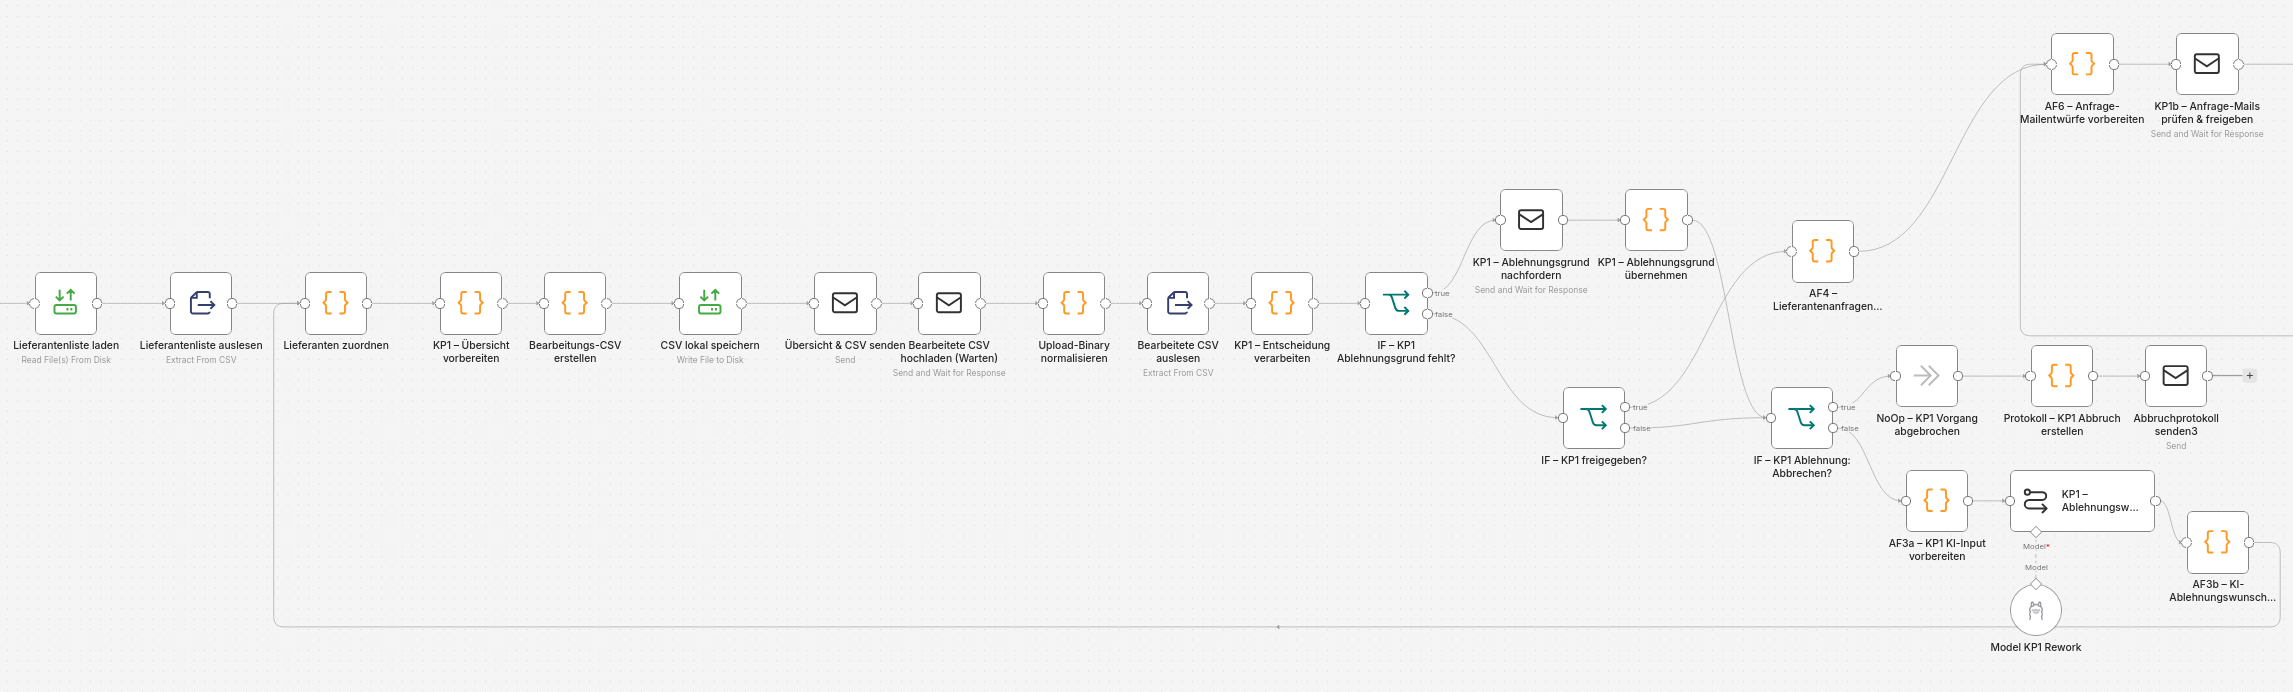
\includegraphics[alt={n8n-Workflow für Lieferantenimport, KP1-Prüfung, CSV-Korrektur und Abbruchpfad},width=\textwidth,height=0.54\textheight,keepaspectratio]{Anhang/n8n-workflowansichten/n8n-02-lieferanten-kp1.png}
    \caption{n8n-Ausschnitt: Lieferantenimport, KP1-Prüfung, CSV-Korrektur und Abbruchpfad}
    \UseTaggingSocket{recordtarget}
    \label{fig:n8n-lieferanten-kp1}
\end{figure}

\paragraph{Freigegebene Anfragen und kontrollierte Angebotsübernahme.}
Eine an KP1 bestätigte Lieferantenzuordnung bildet die Grundlage für lieferantenspezifische Anfrageentwürfe. Innerhalb des KP1-Bereichs prüft ein eigener Mailfreigabeschritt deren Inhalt vor dem Versand. Änderungswünsche am Mailtext können KI-gestützt formuliert werden. Positionen, Mengen, Werkstoffe und Normen müssen dabei unverändert aus den geprüften Daten übernommen werden. Erst die positive Freigabe löst den Versand über SMTP aus. Lieferantenantworten werden im Prototyp über Formular- und Antwortseiten erfasst, damit jede Rückmeldung eindeutig einem Testlauf zugeordnet werden kann.

Die eingehenden Antworten können als Freitext, E-Mail-Text oder strukturierte Eingabe via JSON vorliegen. Der Workflow prüft zunächst, ob daraus bereits belastbare Angebotsdaten abgeleitet werden können. Ist eine KI-Auswertung erforderlich und die Eingabe dafür geeignet, extrahiert der Node \texttt{Lieferantenantwort per KI analysieren} insbesondere Lieferant, Positionsbezug, Menge, Einzelpreis, Lieferkosten, Entladungskosten, Lieferzeit und erkannte Unsicherheiten. Der Fallback \texttt{AF7c2 -- KI überspringen und Fallback nutzen} ergänzt keine fehlenden Inhalte, sondern überführt ausschließlich bereits vorhandene strukturierte Werte in das gemeinsame Angebotsschema. Fehlende Angaben bleiben dadurch für die Vollständigkeitsprüfung sichtbar.

Unklare Preise, Lieferzeiten, Positionen oder Materialbezüge werden der verantwortlichen Person zur fachlichen Klärung vorgelegt. Aus den offenen Punkten erzeugt der Workflow lieferantenspezifische Rückfrage-Mails, die nach Freigabe versendet werden. Eingehende Ergänzungen werden anschließend dem ursprünglichen Antwortdatensatz zugeordnet und erneut der Angebotsprüfung zugeführt. Abbildung~\ref{fig:n8n-antworten-rueckfragen} zeigt diesen Wiedereintrittspfad.

\begin{figure}[H]
    \centering
    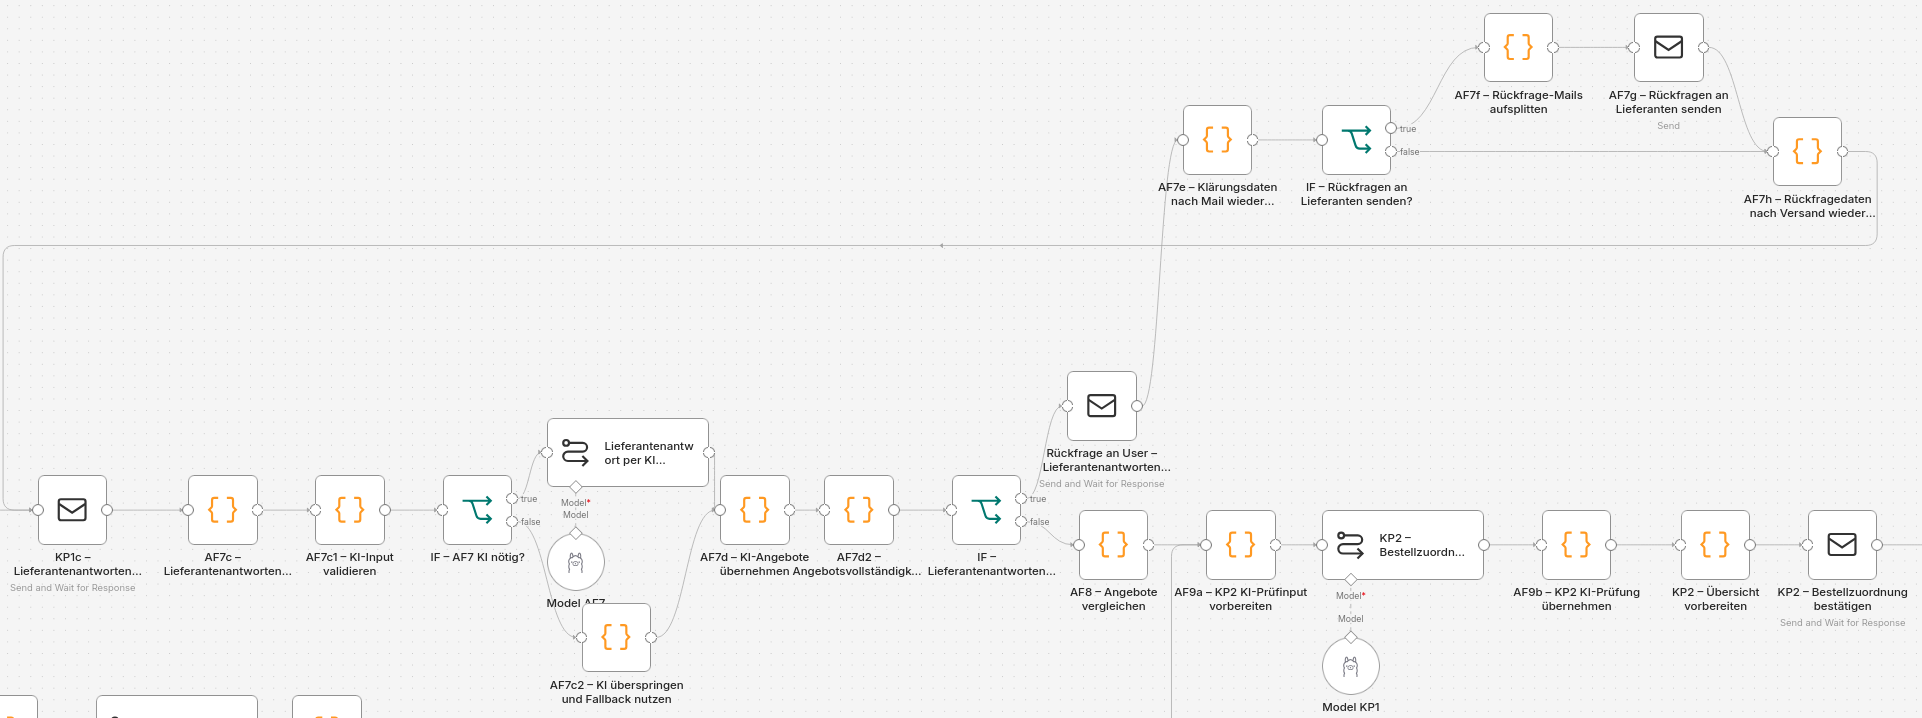
\includegraphics[alt={n8n-Workflow zur Verarbeitung von Lieferantenantworten, KI-Fallbacks, Rückfragen und Bestellzuordnung},width=\textwidth,height=0.54\textheight,keepaspectratio]{Anhang/n8n-workflowansichten/n8n-04-antworten-rueckfragen.png}
    \caption{n8n-Ausschnitt: Verarbeitung der Lieferantenantworten, KI-Fallbacks, Rückfragen und Bestellzuordnung}
    \UseTaggingSocket{recordtarget}
    \label{fig:n8n-antworten-rueckfragen}
\end{figure}

\paragraph{Gesamtkostenvergleich als Grundlage für KP2.}
Aus den übernommenen Angebotsdaten erstellt der Workflow eine Entscheidungsgrundlage. In den Vergleich gehen Stück- beziehungsweise Positionspreise, Lieferkosten, Entladungspauschalen und weitere Zusatzkosten ein. Er berücksichtigt damit die wirtschaftlich relevanten Gesamtkosten und nicht nur den niedrigsten Stückpreis. Eine KI-gestützte Plausibilitätsprüfung kann auf fehlende Angaben oder eine noch nicht belastbare Auswahl hinweisen. Die verbindliche Bestellzuordnung erfolgt jedoch erst an KP2.

Wird an KP2 eine Korrektur verlangt, übernimmt der im Workflow-Export als \texttt{AF10a} bezeichnete Node den Änderungshinweis für die KI-gestützte Überarbeitung. \texttt{AF10b} führt das Ergebnis in die Zuordnungsdaten zurück und schließt damit die technische Korrekturschleife um KP2. Die fachliche Anforderung AF10 betrifft dagegen die anschließende Berechnung des Kostenvoranschlags.

\paragraph{Kostenvoranschlag und Kundenentscheidung.}
Nach der Bestätigung durch KP2 berechnet der Workflow aus den Beschaffungskosten und dem Kalkulationsfaktor die Grundlage für den Kostenvoranschlag. KP3 sichert diesen wirtschaftlich wirksamen Schritt vor der Kundenkommunikation ab. Die anschließende Kundenantwort wird als Zustimmung, kleine Änderung, große Änderung, Ablehnung oder Preisverhandlung eingeordnet.

Eine Zustimmung öffnet den Bestellpfad. Eine kleine Änderung, etwa am Angebotstext oder Liefertermin, führt zur erneuten Freigabe des Kostenvoranschlags. Eine große Änderung betrifft dagegen etwa das Material, die Abmessungen oder neue technische Anforderungen. Sie beendet den aktuellen Lauf kontrolliert und erfordert einen Neustart des betroffenen Prozessabschnitts. Bei einer Ablehnung endet der Vorgang ohne Bestellung. Preisverhandlungen bleiben einer manuellen Klärung vorbehalten. Weder eine KI- noch eine Regelentscheidung erzeugt daher eigenständig eine verbindliche kaufmännische Zusage. Abbildung~\ref{fig:n8n-kundenentscheidung-kp4} zeigt diese Verzweigungen und den Übergang zur Bestellfreigabe.

\begin{figure}[H]
    \centering
    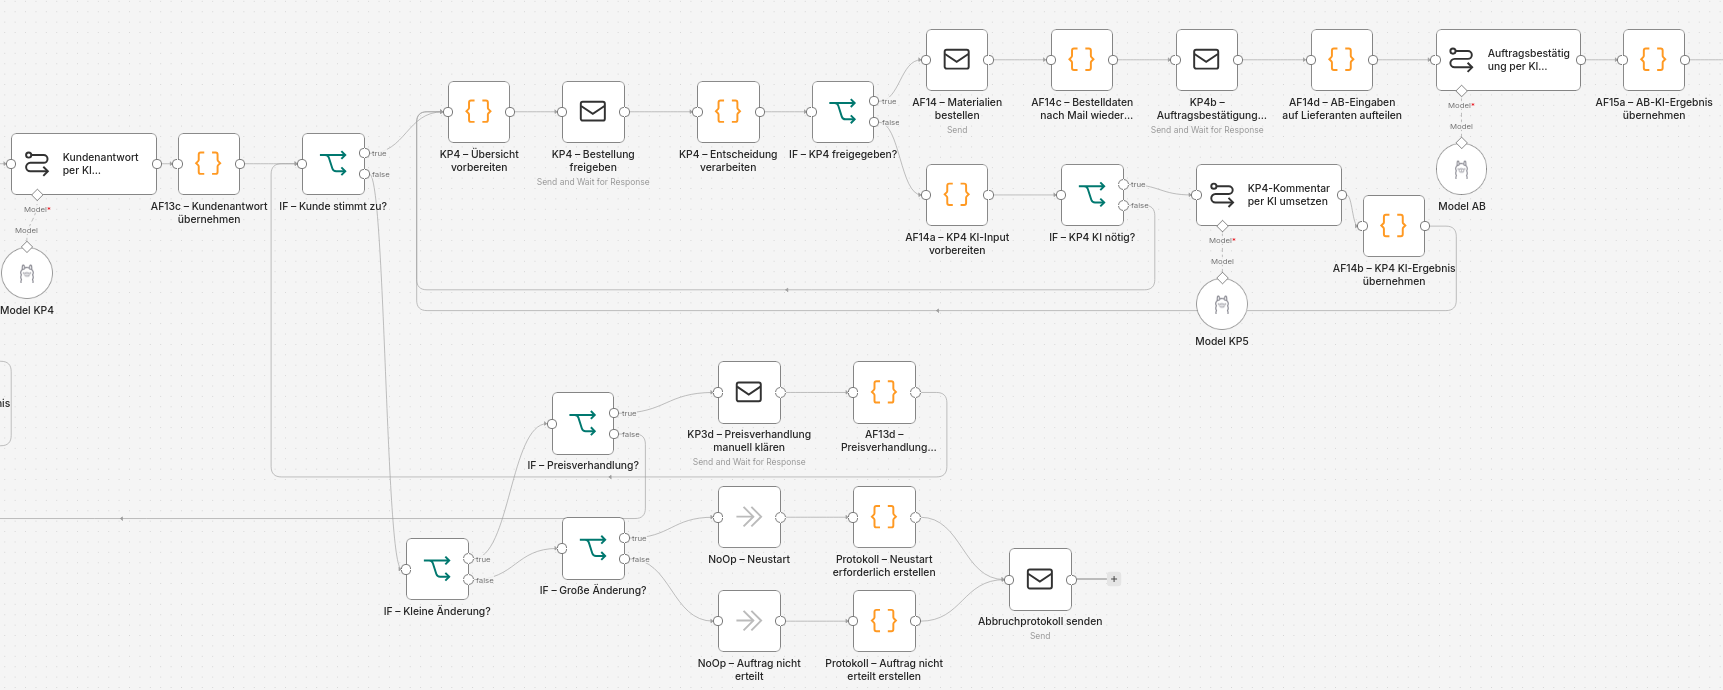
\includegraphics[alt={n8n-Workflow für Kundenentscheidung, Änderungsbehandlung und KP4-Bestellfreigabe},width=\textwidth,height=0.54\textheight,keepaspectratio]{Anhang/n8n-workflowansichten/n8n-06-kundenentscheidung-kp4.png}
    \caption{n8n-Ausschnitt: Kundenentscheidung, Änderungsbehandlung und KP4-Bestellfreigabe}
    \UseTaggingSocket{recordtarget}
    \label{fig:n8n-kundenentscheidung-kp4}
\end{figure}

\paragraph{Bestellung, Auftragsbestätigung und Übergabe.}
Erteilt der Kunde seine Zustimmung, erzeugt der Workflow aus den freigegebenen Daten die Bestell-E-Mails und legt sie KP4 zur letzten Prüfung vor. Ohne eine ausdrückliche Freigabe wird keine Bestellung versendet. Nach dem Versand erfasst der Workflow die \textit{Auftragsbestätigung} (AB). Eine KI-Komponente extrahiert daraus die relevanten Angaben und übergibt die Werte an den Code-Node für den Abgleich mit den Bestelldaten. Geprüft werden insbesondere die Zuordnung zur Bestellung sowie Menge, Preis, Lieferant und Positionsbezug.

Unklare oder abweichende Angaben führen zu einer Klärentscheidung, statt den Prozess automatisch fortzusetzen. Erst nach positiver Prüfung wechselt der Workflow zu \texttt{AF16 -- Auf Lieferung warten}. Dieser Schritt markiert den Übergang zum nicht weiter automatisierten Wareneingang. Abbildung~\ref{fig:n8n-auftragsbestaetigung-protokoll} zeigt die technische Umsetzung der Prüfung und Protokollierung.

\begin{figure}[H]
    \centering
    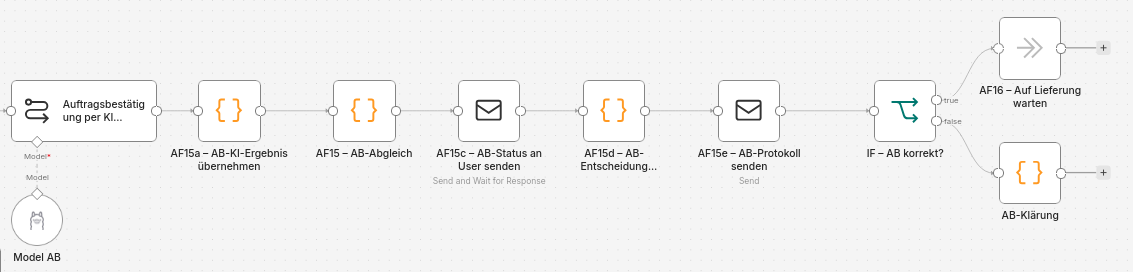
\includegraphics[alt={n8n-Workflow für Auftragsbestätigungsprüfung, Klärentscheidung und Protokollversand},width=\textwidth,height=0.54\textheight,keepaspectratio]{Anhang/n8n-workflowansichten/n8n-07-auftragsbestaetigung.png}
    \caption{n8n-Ausschnitt: Auftragsbestätigungsprüfung, Klärentscheidung und Protokollversand}
    \label{fig:n8n-auftragsbestaetigung-protokoll}
\end{figure}

\paragraph{Phasenübergreifende Nachvollziehbarkeit.}
Über alle Umsetzungsphasen hinweg erzeugt der Prototyp Ausführungsdaten, Debug-Informationen und Statuswerte. Der Node \texttt{Debug -- Lauf initialisieren} legt einen Bezugspunkt für den jeweiligen Prozesslauf an. Weitere Code-Nodes ergänzen Warnungen, Statusinformationen und Protokolleinträge. Die Execution-Ansicht unterscheidet unter anderem fehlgeschlagene, laufende, erfolgreiche und wartende Ausführungen \parencite{n8n_docs_2026}.

Die Freigaben AF17 bis AF20 erscheinen im Workflow-Export nicht als gleichnamige Einzel-Nodes. Sie werden durch das Zusammenspiel von Formular-, Warte-, Entscheidungs- und Rückführungsschritten umgesetzt. Auch Validierung, Protokollierung und definierte Wiedereintrittspunkte beruhen auf mehreren verbundenen Nodes. Wartbarkeit und Datenschutz sind dagegen übergreifende Anforderungen, die nicht allein durch einzelne Workflow-Schritte erfüllt werden. \hyperref[sec:evaluation]{Kapitel~7} bewertet, welche Anforderungen durch die Testläufe und Ausführungsnachweise belegt werden und welche Grenzen bestehen bleiben.

\subsection{Tests und Fehlerbehandlung}
Die technische Prüfung des Prototyps wurde nicht als allgemeiner Funktionstest der Plattform n8n angelegt, sondern entlang der fachlichen Fehlerbilder des SOLL-Prozesses. Grundlage waren die vorbereiteten Testdaten und die in \hyperref[anhang:testprotokolle]{Anhang~\ref*{anhang:testprotokolle}} dokumentierten Testfallprotokolle. Vor jedem Testlauf wurden wartende alte Executions beendet, die passende Stückliste im Node \texttt{Stückliste laden} hinterlegt und die relevanten Ausführungsnachweise gesichert. Dazu gehören die n8n-Execution-ID, die \texttt{debug\_run\_id}, Screenshots der Kontrollpunkte, erzeugte KP1-CSV-Dateien sowie Durchlauf- oder Abbruchprotokolle. Diese Nachweise dienen in \hyperref[sec:umsetzung]{Kapitel~6} vor allem dazu, die technische Fehlerbehandlung nachvollziehbar zu machen. Die bewertende Einordnung der Testergebnisse erfolgt anschließend in \hyperref[sec:evaluation]{Kapitel~7}.

Die Fehlerbehandlung ist im Workflow mehrstufig umgesetzt. Die erste Schutzschicht liegt in der Eingabe- und Stammdatenprüfung. Für die Fehlerbehandlung ist dabei entscheidend, dass ein Prüfstatus den Prozess nicht automatisch fortsetzt, sondern eine Freigabe, Korrektur oder einen kontrollierten Abbruch erzwingt. TF2 prüft diesen Mechanismus anhand einer fehlenden Normangabe. TF3 ergänzt die Stammdatenprüfung um einen bewusst gewählten Negativfall. Die Teststückliste enthält ein Titanrohr aus Titan Grade~2 nach ASTM~B338\footnote{ASTM B338 ist eine technische Spezifikation für nahtlose und geschweißte Rohre aus Titan und Titanlegierungen, insbesondere für Kondensatoren und Wärmeübertrager.}, für das in der vorbereiteten Lieferantenliste keine Bezugsquelle hinterlegt ist. Das Material löst damit gezielt eine fehlende Zuordnung aus. Der Workflow muss die Position offenlassen, statt einen fachlich unpassenden Metalllieferanten auszuwählen.

Die zweite Schutzschicht bilden die Human-in-the-Loop-Kontrollpunkte. KP1 bis KP4 sowie der technische Mailfreigabeschritt KP1b sind als E-Mail-Formulare mit Wartezustand umgesetzt. Die Send-and-Wait-Operation pausiert einen Workflow bis zum Eingang einer Antwort \parencite{n8n_docs_2026}. Im Prototyp führt eine Freigabe in den nächsten Prozessabschnitt. Eine Ablehnung führt je nach Auswahl in einen Abbruchpfad oder in eine Korrekturschleife. Für KP1 wird bei fehlendem Ablehnungsgrund zusätzlich ein Pflichtfeld nachgefordert. Damit wird verhindert, dass ein fachlicher Stopp ohne nachvollziehbare Begründung protokolliert wird. Die Abbruchpfade erzeugen für KP1, KP1b und KP2 eigene Protokolle und senden diese an die hinterlegte E-Mail-Adresse.

Die dritte Schutzschicht betrifft KI-gestützte Schritte. Bei Lieferantenantworten wird der KI-Bedarf nicht durch das Modell selbst, sondern regelbasiert im Node \texttt{AF7c -- Lieferantenantworten verarbeiten} des \hyperref[anhang:n8n-workflow-export]{Workflow-Exports in Anhang~\ref*{anhang:n8n-workflow-export}} bestimmt. Der Node liest zunächst strukturierte JSON-Angaben sowie tabellarisch, abschnittsweise oder als einfacher Antworttext erkennbare Angebotswerte aus. Für jede bekannte Stücklistenposition prüft er, ob ein positiver Preis oder ein eindeutiger Antwortstatus vorliegt. Fehlen alle Parserergebnisse, bleibt mindestens eine Position ohne einen solchen Befund oder erscheint ein automatisch erkannter Preis auffällig, setzt der Node das Feld \texttt{ki\_noetig} auf \texttt{true}. Als auffällig gilt der Wert des einfachen Textparsers, wenn der erkannte positive Preis höchstens 1 beträgt oder ein weiterer Geldbetrag im Text mindestens fünfmal so hoch ist. Ein strukturierter JSON-, Tabellen- oder Abschnittswert mit positivem Preis hebt diesen Verdacht auf.

Vor der Verzweigung prüft \texttt{AF7c1 -- KI-Input validieren}, ob mindestens eine Antwortmail vorliegt, deren zusammengeführter Text nach der Bereinigung mindestens 20 Zeichen umfasst. Zusätzlich muss wenigstens ein Positionsbezug vorhanden sein. Bei unzureichenden Eingaben bricht der Workflow mit einer Fehlermeldung ab. Sind die Mindestbedingungen erfüllt, führt \texttt{IF -- AF7 KI nötig?} nur Läufe mit \texttt{ki\_noetig=true} in die LLM-Kette. Andernfalls leitet der Node den Lauf an \texttt{AF7c2 -- KI überspringen und Fallback nutzen} weiter. Die bereits erkannten Werte bleiben dabei unverändert erhalten. Beide Pfade münden in \texttt{AF7d -- KI-Angebote übernehmen}, der die KI- und Fallbackdaten in ein gemeinsames Angebotsschema überführt. Die anschließende regelbasierte Vollständigkeitsprüfung führt unklare oder fehlende Angaben über Rückfrage-Mails und eine erneute Antworterfassung in den definierten Wiedereintrittspunkt.

Die vierte Schutzschicht liegt im Abgleich der Auftragsbestätigung. \texttt{Auftragsbestätigung per KI analysieren} extrahiert Angaben aus der Rückmeldung. \texttt{AF15 -- AB-Abgleich} vergleicht die übergebenen Felder mit der Bestellung. Die Regelprüfung ist damit von der Qualität der vorgelagerten Extraktion abhängig. Bei unklaren oder abweichenden Angaben kann der Workflow über \texttt{AF15c -- AB-Status an User senden}, \texttt{AF15d -- AB-Entscheidung übernehmen} und \texttt{IF -- AB korrekt?} eine menschliche Entscheidung anfordern. AF15 ist deshalb als Vorprüfung mit Klärzweig zu verstehen. Ein zuverlässiger automatischer Mengen- und Preisabgleich oder eine zuverlässige Zuführung aller kritischen Dokumente in diesen Zweig wird durch die Testläufe nicht belegt.

Für technische Laufzeitfehler ist ein separater Fehlerworkflow (Error Workflow) vorgesehen. n8n führt einen zugeordneten Error Workflow aus, wenn eine Workflow-Ausführung fehlschlägt \parencite{n8n_docs_2026}. Im Artefakt erzeugt dieser Workflow ein Fehlerprotokoll, ersetzt aber nicht die fachlichen Abbruch- und Klärpfade des Hauptworkflows. Fachliche Abweichungen werden über Validierungen, IF-Knoten, Formularfreigaben und Klärschleifen behandelt. Technische Fehler werden über Execution-Daten und den Fehlerworkflow sichtbar gemacht. Der Prototyp verbindet Code-Nodes, Freigaben, Fallbacks und Protokolle zu einer mehrstufigen Fehlerbehandlung. AF15 bleibt wegen der Abhängigkeit von der KI-Extraktion eine Vorprüfung mit menschlichem Klärpfad. Die Zuordnung dauerhafter Support- und Wartungsverantwortung ist eine organisatorische Betriebsaufgabe \parencite{herm_framework_2023}.

\clearpage
\section{Evaluation}
\label{sec:evaluation}
Die Evaluation bewertet den Prototyp anhand der definierten Testfälle und Kriterien. Dadurch wird sichtbar, welche Anforderungen in den ausgewählten Testpfaden nachgewiesen werden, wo manuelle Kontrolle notwendig bleibt und welche Risiken für eine spätere Produktivlösung bestehen.

\subsection{Evaluationsdesign}
Die Evaluation bewertet das entwickelte Artefakt anhand der zuvor festgelegten Kriterien und dokumentierten Nachweise. \Textcite{peffers_design_2007} beschreiben dafür den Vergleich der Lösungsziele mit den beobachteten Ergebnissen. Für den vorliegenden Fall wird dieser methodische Schritt durch fünf fallnahe Testfälle umgesetzt. Bewertet wird nicht, ob der Prototyp bereits produktionsreif ist, sondern ob die im SOLL-Prozess definierte Prozesslogik technisch abbildbar ist und typische Fehlerfälle kontrolliert behandelt werden. Die Testfälle TF1 bis TF5 untersuchen dazu einen Referenzpfad und gezielte Ausnahmen. TF1 erreichte den technischen Pfad bis AF16 und belegt damit dessen vollständige Ausführung und Protokollierung.

Die Zuordnung der fünf Testfälle zu Prozessrisiken und Bewertungskriterien ist in \hyperref[sec:evaluationslogik]{Abschnitt~\ref*{sec:evaluationslogik}} und im Kriterienrahmen begründet. Die Evaluation stützt sich auf die tatsächlich erreichten Ausführungspfade und beurteilt deren Nachweisqualität, Abweichungen und Grenzen. Die Testläufe dienen damit als strukturierte Prüfung der Prozesslogik, der Fehlerbehandlung und der menschlichen Kontrollpunkte, nicht als produktiver Leistungsnachweis.

Jeder Testfall wird mit Eingabe, erwartetem Ergebnis, tatsächlichem Ergebnis, Ausführungsnachweis und Abweichungen dokumentiert. Die Ausführungsnachweise bestehen aus den dokumentierten n8n-Execution-IDs, den Debug-Run-IDs, den erzeugten Durchlauf- beziehungsweise Abbruchprotokollen sowie Screenshots der relevanten Kontrollpunkte. Für TF1, TF4 und TF5 liegen vollständige Durchlaufprotokolle mit Debug-Run-ID vor. TF2 und TF3 endeten beide planmäßig an KP1, lösten dort jedoch unterschiedliche fachliche Prüfhinweise aus. TF2 wurde wegen der fehlenden Normangabe abgelehnt, TF3 wegen der fehlenden Lieferantenzuordnung. Die Abbruchprotokolle halten die jeweilige Ablehnung, KP1 als Abbruchstelle und den fachlichen Grund fest. Ein vollständiger Debug-Trace liegt für diese beiden Testfälle nicht vor.

Der Workflow-Export und die Testprotokolle erfüllen unterschiedliche Nachweisfunktionen. Der Export dokumentiert die technisch angelegten Funktionen für den Versand von Lieferantenanfragen (AF5), das Warten auf Lieferantenantworten (AF6), den Versand des Kostenvoranschlags (AF11), die Verarbeitung der Kundenentscheidung (AF12) und den Versand freigegebener Bestellungen (AF14). Er belegt damit die vorhandene Workflow-Struktur, nicht jedoch deren vollständige Ausführung. Die Testprotokolle weisen dagegen nur die tatsächlich durchlaufenen Prozesspfade nach. Lieferanten- und Kundenreaktionen wurden manuell in den Workflow übergeben. AF16 beschreibt das Warten auf die Lieferung und die anschließende Übergabe an den manuellen Wareneingang. Im Prototyp ist diese Anforderung lediglich als \texttt{NoOp}-Übergabemarkierung umgesetzt. NF4 zur Wartbarkeit und NF5 zu Datenschutz und Datenhoheit werden strukturell eingeordnet, jedoch nicht durch eigenständige Testfälle geprüft.

KP1 bis KP4 sind fachliche Human-in-the-Loop-Kontrollpunkte und keine Kennzahlen. Durchlaufzeiten wurden nicht erhoben, da Lieferanten- und Kundenreaktionen simuliert oder manuell fortgesetzt wurden und weder ein vergleichbarer IST-Wert noch wiederholte Messläufe vorlagen. Auch die Zahl manueller Eingriffe wurde nicht als Kennzahl erfasst, weil verpflichtende Freigaben und zusätzliche Korrektureingriffe vor den Tests nicht als getrennte Messgrößen festgelegt waren.

Eine prozentuale Anforderungsabdeckung wird ebenfalls nicht ausgewiesen. Die fünf risikobasiert ausgewählten Testfälle bilden keinen vollständigen Abnahmetest aller 25 Anforderungen von AF1 bis AF20 und NF1 bis NF5. Die Datenvollständigkeit liegt nur als knoten- und testfallspezifischer Wert vor. Die in TF5 ausgewiesenen \(0\,\%\) beziehen sich beispielsweise auf die Extraktion der Auftragsbestätigung und nicht auf die Datenqualität des Gesamtprozesses. Die vier Größen liegen daher nicht als einheitlich erhobene, prozessweite Messergebnisse vor.

\subsection{Ergebnisse der Testfälle und Bewertungskriterien}
Die Testläufe dokumentieren die jeweils erreichten Standard- und Fehlerpfade des Prototyps sowie die weiterhin notwendige menschliche Kontrolle. Die folgenden Ergebnisse beruhen auf den in \hyperref[anhang:testprotokolle]{Anhang~\ref*{anhang:testprotokolle}} dokumentierten Testfallprotokollen. Bewertet werden die Kriterien funktionale Abdeckung, Datenqualität, Human-in-the-Loop, Kostenberechnung, Fehlerbehandlung und Protokollierbarkeit.

\begin{table}[H]
    \captionsetup{justification=raggedright,singlelinecheck=false}
    \caption{Ergebnisse der Testfälle TF1 bis TF5}
    \label{tab:testfallergebnisse}
    \footnotesize
    \begin{tabularx}{\textwidth}{@{}lXX@{}}
        \toprule
        Testfall & Kernbefund & Einordnung \\
        \midrule
        TF1 & Prozesskette abgeschlossen. KP3 berechnete 1.884,20~EUR Beschaffungskosten und 2.449,46~EUR Kostenvoranschlag. & Bestanden für den technischen Referenzpfad und die Protokollierung. \\
        TF2 & Die fehlende Norm wurde an KP1 als \enquote{offen/prüfpflichtig} erkannt und angezeigt. Anschließend wurden \enquote{ablehnen} und \enquote{abbrechen} ausgewählt. & Bestanden, weil die fehlende Angabe sichtbar wurde und der Lauf an KP1 im vorgesehenen Abbruchpfad endete. \\
        TF3 & Für die Position wurde keine Lieferantenzuordnung erzeugt. KP1 zeigte den Fall als \enquote{offen/prüfpflichtig} an. & Bestanden, weil kein fachlich falscher Treffer erzeugt wurde. \\
        TF4 & Bei gleichem Stückpreis wurde wegen geringerer Liefer- und Entladungskosten \enquote{Stahlhandel-Nord} gewählt. KP3 ergab 299,00~EUR Kostenvoranschlag. Der Angebotsimport nutzte strukturierte Fallback-Daten und keinen KI-Pfad. & Bestanden für den Zusatzkostenvergleich. \\
        TF5 & Eine bewusst abweichende Auftragsbestätigung wurde als \enquote{unklar} eingestuft und nach menschlicher Klärung als \enquote{nicht korrekt} protokolliert. & Bestanden für den Schutztest, weil die fehlerhafte Eingabe nicht automatisch akzeptiert wurde. \\
        \bottomrule
    \end{tabularx}
\end{table}

Die Testfallkombination dokumentiert für den abgegrenzten Proof of Concept die grundsätzliche Ausführbarkeit ausgewählter Standard- und Fehlerpfade. AF1 bis AF16 werden nicht in jedem Testfall vollständig durchlaufen. Belegt sind die jeweils in den Protokollen und Screenshots ausgewiesenen Teilpfade für Stücklistenimport, Validierung, Lieferantenzuordnung, Lieferantenanfragen, Angebotsübernahme, Kostenvergleich, Kostenvoranschlag, Bestellung und Auftragsbestätigung. AF17 bis AF20 werden in den jeweils erreichten Formularentscheidungen sichtbar. Bei TF2 kennzeichnete die Validierung die fehlende Norm als \enquote{offen/prüfpflichtig}. KP1 hielt den Lauf bis zur vorgesehenen Entscheidung an. Nach der Auswahl von \enquote{ablehnen} und \enquote{abbrechen} führte der Workflow den dokumentierten Abbruchpfad aus. In TF3 blieb die Lieferantenzuordnung leer, sodass kein fachlich falscher Treffer entstand. Der ebenfalls dokumentierte Abbruch an KP1 bestätigt die kontrollierte Behandlung, ist aber nicht das zentrale Prüfkriterium dieses Testfalls.

Die Datenqualität bleibt der zentrale Engpass. TF2 zeigt, dass fehlende Normangaben früh erkannt werden können. TF3 zeigt, dass fehlende Stammdaten in der Lieferantenliste nicht durch Scheintreffer ersetzt werden. TF4 belegt die Berücksichtigung von Liefer- und Entladungskosten. Der vollständige technische Prozesspfad einschließlich AF15 ist bereits durch TF1 belegt. TF5 prüft ergänzend die Schutzwirkung bei einer bewusst fehlerhaften Eingabe. Dazu wurde eine Auftragsbestätigung verwendet, deren Menge 7 und Positionspreis von 420,00~EUR von den Bestelldaten abwichen. Die automatische Prüfung konnte diese Angaben nicht belastbar der Materialposition zuordnen und bewertete die erkannte Datenvollständigkeit mit \(0\,\%\). Der Status blieb deshalb \enquote{unklar} und der Workflow forderte eine Klärentscheidung an. Die verantwortliche Person stufte die Bestätigung als \enquote{nicht korrekt} ein. TF5 belegt somit, dass eine unsichere Eingabe nicht automatisch freigegeben wird.

Die Protokollierbarkeit ist für die Evaluation ausreichend. TF1, TF4 und TF5 enthalten vollständige Durchlaufprotokolle, Warnungen und finale Statuswerte. TF2 und TF3 enthalten Abbruchprotokolle mit Abbruchstelle und Begründung. Damit lassen sich die in den erreichten Testpfaden nachgewiesenen Anforderungen, die erkannten Fehlerfälle und die dokumentierten manuellen Entscheidungen nachvollziehen. Ein produktiver Audit-Trail wäre damit noch nicht erreicht, da Rollen, Benutzeridentitäten, Aufbewahrungsfristen und manipulationssichere Protokollierung nicht umgesetzt sind. Für den Proof of Concept reicht die vorhandene Dokumentation allerdings aus, um die Prozesslogik und die Behandlung der Testfälle nachvollziehbar zu bewerten.

\subsection{Diskussion der Grenzen, Risiken und Übertragbarkeit}
Die Ergebnisse sind auf den untersuchten Fallbetrieb und den kontrollierten Testaufbau begrenzt. Die Testläufe dokumentieren ausgewählte Prozesspfade von der Stückliste bis zur Auftragsbestätigung. Sie erlauben jedoch keine Aussage darüber, ob ein kleiner Handwerksbetrieb den Workflow dauerhaft produktiv betreiben kann. Die in \hyperref[sec:prototyp-produktiv]{Abschnitt~\ref*{sec:prototyp-produktiv}} beschriebenen Voraussetzungen für Organisation, technischen Betrieb, Datenschutz und Wartung wurden im Proof of Concept nicht vollständig umgesetzt oder geprüft. Die Evaluation beurteilt daher die Prozesslogik und ausgewählte Fehlerpfade, nicht die Betriebsfähigkeit einer Produktivlösung.

Ein wesentliches Risiko liegt im hohen Anteil eigener Code-Logik. Die 57 Code-Nodes ermöglichen eine genaue Anpassung an den untersuchten Beschaffungsprozess, erhöhen jedoch die Abhängigkeit von technischem Wissen und einzelnen verantwortlichen Personen. Für vergleichbare KKU ist daher nicht nur die einmalige Entwicklung, sondern vor allem die spätere Pflege kritisch. Lieferantenregeln, Kostenfaktoren, Formulare und Mailvorlagen können sich im Betrieb verändern. Die Implementierungsliteratur ordnet Support, Wartung und klare Rollen als fortlaufende Aufgaben ein \parencite{herm_framework_2023}. Für den vorliegenden Fall wird daraus abgeleitet, interne Kompetenz aufzubauen oder eine externe Betreuung verbindlich zu regeln. Low-Code erleichtert den Einstieg, ersetzt aber keine Verantwortung für Geschäftsregeln, Datenqualität und Betrieb.

Auch die Benutzerführung bleibt prototypisch. E-Mail-Formulare eignen sich für kontrollierte Tests, bilden jedoch keine ausgereifte Benutzeroberfläche. Für einen Produktivbetrieb müssten Formulare, Antwortketten und die Zuordnung zu den jeweiligen Beschaffungsvorgängen belastbarer gestaltet werden. Bei Kundenantworten wäre insbesondere zu prüfen, ob sich die Rückmeldung anhand von Betreff, Projektbezug, Materialpositionen und Kosten eindeutig dem richtigen Kostenvoranschlag zuordnen lässt.

Die Befunde zur KI-gestützten Verarbeitung sind nur eingeschränkt auf andere Eingaben, Modelle und Prozesssituationen übertragbar. Strukturierte JSON-Felder, eng gefasste Prompts und die Beschränkung auf assistierende Aufgaben reduzieren den Handlungsspielraum des Modells, gewährleisten jedoch keine quellentreue Verarbeitung. Sprachmodelle können falsche oder nicht durch die Eingabe gestützte Ausgaben erzeugen. \Textcite{farquhar_detecting_2024} bezeichnen solche falschen oder unbelegten Modellausgaben als Halluzinationen. Sie untersuchen ein Verfahren, das inhaltliche Unsicherheit nutzt, um frei erfundene Antworten als besondere Form solcher Halluzinationen zu erkennen. Ob die im Prototyp beobachteten Fehler dieser Form von Halluzination zuzuordnen sind, lässt sich aus einzelnen Testläufen nicht bestimmen. Für die Fallbefunde sind daher die Bezeichnungen \enquote{inhaltliche Fehlklassifikation} und \enquote{Extraktionsfehler} präziser.

Für die Diskussion bleiben aus diesen Testbefunden zwei übergreifende Grenzen relevant. Fehlende Herkunfts- und Eingangsdaten erschweren die nachträgliche Prüfung einzelner Einstufungen. Außerdem wurden vorhandene Mengen- und Preisangaben in einzelnen Läufen nicht belastbar der zugehörigen Materialposition zugeordnet. Die Kontroll- und Klärpfade verhinderten zwar eine automatische Fortsetzung, ersetzen jedoch keine zuverlässige Prüfung von Dokumenttyp, Herkunft und extrahierten Daten.

Die Beschränkung auf kleine, lokal ausführbare Modelle begrenzt die Übertragbarkeit der Ergebnisse auf größere Modelle und leistungsfähigere Hardware. Fünf Testläufe erlauben keine Aussage über den Zusammenhang zwischen Modellgröße und Fehlerrate. Dafür wären wiederholte Versuche mit mehreren Modellen und identischen Eingaben erforderlich. Der Fallbefund zeigt nur, dass auch eng geführte kleine Modelle vorhandene Angaben übersehen oder inhaltlich unzutreffend einordnen können. Dokumenttypprüfung, deterministische Vergleiche, Fallbacks und menschliche Freigaben bleiben daher notwendig. Für den vorliegenden Fall wird aus den Testbefunden und dem in der Literatur beschriebenen Human-in-the-Loop-Prinzip abgeleitet, KI produktiv nur bei begrenzten Fehlerfolgen und nachgelagerter Prüfbarkeit einzusetzen \parencite{ng_systematic_2021}.

Im Prüfaufbau wurden n8n, Prozessdateien, Protokolle und Ollama auf dem eigenen System betrieben. Dadurch erhielt kein externer KI-Anbieter die Modelleingaben. Daraus folgt jedoch keine allgemeine Sicherheit lokaler Verarbeitung. Ungeeignete Rechte, Fehlbedienung, unsichere Zugangsdaten, ungeschützte Sicherungen und falsch konfigurierte Zugriffe auf E-Mail- oder Formularfunktionen bleiben mögliche Betriebsrisiken. Der n8n-Security-Audit kann ausgewählte Konfigurationsrisiken wie ungenutzte Credentials, Nodes mit Dateisystemzugriff, risikobehaftete Nodes und ungeschützte Webhooks sichtbar machen \parencite{n8n_docs_2026}. Die n8n-Kommandozeilenschnittstelle (\textit{Command Line Interface}, CLI) unterstützt den Export und Import von Workflows und Credentials und stellt damit technische Bausteine für Sicherung und Wiederherstellung bereit \parencite{n8n_docs_2026}. Diese Funktionen ersetzen jedoch kein geprüftes Sicherungs- und Wiederherstellungskonzept. Sofern personenbezogene Daten verarbeitet werden, müssen zusätzlich Speicherung, Zugriff, Aufbewahrung und Löschung anhand der DSGVO geregelt werden \parencite{eu_dsgvo_2016}. Für den vorliegenden Fall wird daraus abgeleitet, auch geschäftliche Daten ohne Personenbezug in das Sicherheits- und Betriebskonzept einzubeziehen.

Auf vergleichbare KKU übertragbar sind vor allem das methodische Vorgehen, die Trennung zwischen automatisierten und menschlich freizugebenden Schritten sowie die Behandlung typischer Fehlerfälle. Die konkrete Workflow-Struktur, Lieferantenlogik, Datenfelder und KI-Konfiguration können dagegen nicht unverändert übernommen werden. Sie müssen an den jeweiligen Beschaffungsprozess, die vorhandenen Systeme, die Datenqualität und die betrieblichen Zuständigkeiten angepasst werden.

\clearpage
\section{Fazit und Ausblick}
\subsection{Beantwortung der Forschungsfragen}
Die Leitfrage lässt sich anhand einer begrenzten, im Prüfaufbau nachgewiesenen Teilautomatisierung beantworten. Die Arbeit verbindet die Erhebung des IST-Prozesses, seine Schwachstellenpriorisierung und den daraus entwickelten SOLL-Prozess mit einem ausführbaren n8n-Prototyp. Wiederkehrende Beschaffungsschritte können dadurch in einem gemeinsamen Datenfluss vorbereitet, geprüft und dokumentiert werden. Wirtschaftlich wirksame Entscheidungen bleiben an menschliche Freigaben gebunden. Nachgewiesen ist somit die technische Ausführung des abgegrenzten Prozesses, aber keine einsatzbereite Produktivlösung.

Die IST-Analyse beantwortet die erste Teilfrage nach den Schwachstellen des bestehenden Materialbeschaffungsprozesses. Den größten Handlungsbedarf erzeugen unvollständige Materialdaten, weil sich daraus Fehler bis in späte Prozessphasen fortsetzen können. Hinzu kommen die Abhängigkeit von personengebundenem Lieferantenwissen und die späte Erkennung von Abweichungen in Auftragsbestätigungen. Uneinheitliche Angebotsvergleiche, lange Antwortzeiten, schwer nachvollziehbare Entscheidungen und Rücksprünge nach Kundenänderungen ergänzen das Schwachstellenbild. Die fallbezogene Priorisierung zeigt, dass eine Automatisierung zuerst Datenqualität und Nachvollziehbarkeit verbessern sollte, bevor sie weitere Entscheidungen nach außen trägt.

Aus diesen Befunden folgen für die zweite Teilfrage die Anforderungen an den automatisierten SOLL-Prozess. Der SOLL-Prozess prüft Materialangaben früh, macht Lieferantenwissen über strukturierte Daten verfügbar und vergleicht Angebote anhand der Gesamtkosten. Der Zusammenhang zeigt sich beispielsweise bei unvollständigen Materialangaben. Weil diese Fehler bisher erst spät auffallen, werden die Angaben nun unmittelbar nach dem Import vereinheitlicht, kategorisiert und validiert. Personengebundenes Lieferantenwissen wird entsprechend über eine gepflegte Lieferantenliste und eine nachvollziehbare Zuordnungslogik zugänglich gemacht. Lieferantenanfragen, Kostenvoranschläge und Bestellungen werden erst nach einer fachlichen Freigabe weitergegeben. Eigene Klär- und Rückführungspfade greifen Kundenänderungen und Abweichungen in Auftragsbestätigungen auf. Protokollierung, Wartbarkeit und Datenschutz ergänzen den SOLL-Prozess als übergreifende Anforderungen. Die Anforderungen führen die Ergebnisse der IST-Analyse damit in ein prüfbares Prozesskonzept über.

Die prototypische Umsetzung und Erprobung des SOLL-Prozesses mit n8n beantwortet die dritte Teilfrage. n8n verbindet den Stücklistenimport, die Datenprüfung, Lieferantenzuordnung, Angebotsverarbeitung, Freigaben, Bestellung und Bestätigungsprüfung in einem ausführbaren Workflow. Dateien, E-Mail-Formulare, eigene Code-Logik und die lokale Ollama-Instanz bilden gemeinsam die Architektur. Der vorgesehene Referenzpfad erreichte im Prüfaufbau die Übergabe an den manuellen Wareneingang. Die Ausführungsnachweise zeigen außerdem, dass fehlende Normangaben und Lieferantenzuordnungen sichtbar werden, fachlich falsche Lieferantentreffer ausbleiben und Zusatzkosten in den Angebotsvergleich eingehen. Unsicherheiten bei der Bestätigungsprüfung begrenzen jedoch die Bewertung des Referenzpfads als durchgängig fehlerfreien Prozessnachweis. Die Kontroll- und Klärpfade verhinderten dennoch eine unbemerkte automatische Fortsetzung. Die Testfälle ergänzen damit Workflow-Export, Prozessmodell und Protokolle als Nachweise, bilden aber nicht allein die Grundlage der Bewertung.

Die vierte Teilfrage betrifft die Voraussetzungen und Risiken eines möglichen Produktivbetriebs. Der lokale Prüfaufbau begrenzte die Weitergabe von Daten an externe Dienste, ließ jedoch technische, organisatorische und wirtschaftliche Voraussetzungen eines dauerhaften Betriebs offen. Dazu zählen abgesicherte Zugänge, klare Zuständigkeiten, verlässliche Betriebsprozesse und die dafür erforderlichen internen oder externen Ressourcen. Bei der Verarbeitung personenbezogener Daten sind zusätzlich datenschutzrechtliche Anforderungen zu prüfen \parencite{eu_dsgvo_2016}.

Der untersuchte Fall zeigt, dass n8n für klar abgegrenzte, regelbasierte und ausreichend strukturierte Beschaffungsschritte grundsätzlich geeignet sein kann. Der Prototyp zeigt, wie Prüfungen vorgezogen, Daten für nachfolgende Schritte strukturiert bereitgestellt und Entscheidungen nachvollziehbarer dokumentiert werden können. Betriebliches Beschaffungswissen und verantwortliche Entscheidungen werden dabei unterstützt, aber nicht ersetzt. Diese Ergebnisse bilden die Grundlage der \hyperref[sec:handlungsempfehlungen-kku]{Handlungsempfehlungen für vergleichbare KKU}.

\subsection{Handlungsempfehlungen für KKU}
\label{sec:handlungsempfehlungen-kku}
Die Handlungsempfehlungen sind als Transferhypothesen für vergleichbare materialverarbeitende KKU mit weniger als zehn Mitarbeitenden, manuell geprägter Beschaffung und datei- sowie E-Mail-basierter IT zu verstehen. Sie bilden eine eigene Synthese aus Fallanalyse, Prototyp, Testbefunden und Literatur. Ihre Übertragbarkeit auf andere Unternehmensgrößen, Branchen oder Reifegrade muss erneut geprüft werden.

Die untersuchten Fehlerfälle zeigen, dass unvollständige Pflichtangaben und fehlende Lieferantenzuordnungen früh erkennbar sein müssen. Vergleichbare KKU sollten deshalb die in ihrem Prozess benötigten Stücklistenattribute und Lieferantenstammdaten vor der Automatisierung verbindlich festlegen. Nicht verfügbare Angaben dürfen nicht durch Scheintreffer oder Standardwerte verdeckt werden, sondern müssen als offene Klärpunkte erhalten bleiben.

Aus den Befunden der \hyperref[sec:evaluation]{Evaluation} folgt, dass Auftragsbestätigungen eindeutig einem Vorgang zugeordnet und ihre Herkunft nachvollziehbar dokumentiert werden sollten. Eine durchgängige Vorgangs-ID sollte die Bestätigung mit der Bestellung und dem Prozesslauf verbinden. In der Freigabeansicht sollten Herkunft, Bestellwerte und extrahierte Angaben nachvollziehbar gegenübergestellt werden. So bleiben fehlerhaft übernommene Werte für die verantwortliche Person erkennbar.

TF4 zeigt im Prüfaufbau, dass ein Angebotsvergleich neben dem Stückpreis auch Lieferkosten, Entladungspauschalen und weitere Zusatzkosten berücksichtigen muss. Bei gleichem Stückpreis kann ein Angebot durch niedrigere Liefer- und Entladungskosten insgesamt günstiger sein. Die Kontrollpunkte zeigen zugleich, an welchen Stellen eine fachliche Freigabe erforderlich bleibt. Freigabeansichten sollten daher die verwendeten Kostenbestandteile, offene Angaben und die Außenwirkung der Entscheidung gemeinsam darstellen. So können Lieferantenanfragen, Kostenvoranschläge und Bestellungen vor ihrer Freigabe nachvollziehbar geprüft werden.

Vor einem Produktivbetrieb ist ein tragfähiges Betriebs- und Kostenmodell festzulegen. Im untersuchten Fall umfasst die Kostenbetrachtung Hardware- oder Hostingkosten, Einrichtungsaufwand, interne Lernzeit, laufende Wartung und mögliche externe Unterstützung. \Textcite{mostaquim_study_2022} setzt in einem Kostenvergleich für Open-Source-RPA Wartungsaufwand an und behandelt den Bedarf an Fachkompetenz und Personal. Der Wartungsansatz ist dort eine Annahme und kein empirisch gemessener Aufwand. \Textcite{asatiani_deciding_2023} unterscheiden Entscheidungen über interne oder externe Ressourcen, lokale oder cloudbasierte Bereitstellung sowie proprietäre oder offene Werkzeuge.

Daraus wird für den untersuchten Fall abgeleitet, die gewählte Bereitstellung auf die gewünschte Datenhaltung, die verfügbaren Kompetenzen und die dauerhaft übernommenen Betriebsaufgaben abzustimmen. Der hohe Anteil eigener Code-Logik und das lokale Setup erzeugen einen fortlaufenden Pflegebedarf. Vor dem Produktivbetrieb sind deshalb die Zuständigkeiten für technische Änderungen, fachliche Prüfungen und die Freigabe neuer Workflow-Versionen festzulegen. Ist intern keine ausreichende Kompetenz vorhanden, sollte der Umfang externer Unterstützung für Wartung und Tests verbindlich festgelegt werden. Auch die Verantwortung für diese Betriebsaufgaben muss eindeutig zugeordnet sein.

Ein verlässlicher Betrieb erfordert Schutz- und Wiederanlaufmaßnahmen. Zugriffsrechte für E-Mail-Konten sind zu dokumentieren. Zugleich müssen Regeln und in n8n gespeicherte Zugangsdaten gegen unbefugte Änderungen geschützt werden. Regelmäßige Sicherungen und erprobte Wiederherstellungswege begrenzen die Folgen eines Systemausfalls oder einer fehlerhaften Änderung. Die n8n-CLI stellt Export- und Importfunktionen für Workflows und Credentials bereit \parencite{n8n_docs_2026}. Im untersuchten Fall bilden diese Funktionen technische Bausteine für Sicherung und Wiederherstellung.

Auch Aktualisierungen sollten zunächst in einer getrennten Testumgebung geprüft werden. Die offizielle Dokumentation empfiehlt regelmäßige Updates, die Prüfung der Release Notes und vorgelagerte Tests in einer Testinstanz \parencite{n8n_docs_2026}. Ändert ein Lieferant beispielsweise seine Lieferpauschale oder das Format einer Angebotsmail, sollte die Anpassung zunächst in einer Testkopie erfolgen. Vor der Freigabe sollten mindestens der Zusatzkostenvergleich und ein relevanter Fehlerfall erneut geprüft werden. Dadurch lässt sich kontrollieren, ob Gesamtkostenberechnung und Ausnahmebehandlung weiterhin funktionieren.

Datenschutzrechtliche Anforderungen sind zu prüfen, soweit personenbezogene Daten verarbeitet werden. Das betrifft etwa Namen, persönliche Kontaktdaten oder personenbezogene E-Mail-Inhalte. Reine Material- und Preisangaben ohne Bezug zu einer natürlichen Person machen eine solche Prüfung nicht allein erforderlich. Bei personenbezogenen Daten sind insbesondere Aufbewahrung, Löschung, Zugriffsschutz und gegebenenfalls die Auftragsverarbeitung für den jeweiligen Betrieb nachvollziehbar zu regeln \parencite{eu_dsgvo_2016}.

\subsection{Ausblick}
Der nächste Entwicklungsschritt ist die technische Verfeinerung der in den \hyperref[sec:handlungsempfehlungen-kku]{Handlungsempfehlungen} abgeleiteten Eingangskontrolle für Auftragsbestätigungen. Ihre Zuverlässigkeit sollte anschließend mit unterschiedlichen Dokumentformaten wiederholt geprüft werden. Im Mittelpunkt stehen die korrekte Vorgangszuordnung, die Qualität der Extraktion und der regelbasierte Vergleich mit den Bestelldaten. Das Sprachmodell soll dabei ausschließlich unstrukturierte Inhalte in ein vorgegebenes Schema überführen. Vollständigkeit, Datentypen und fachliche Abweichungen sind anschließend deterministisch zu prüfen.

Darauf aufbauend bietet sich eine begrenzte Erprobungsphase mit einer Materialgruppe, regelmäßig genutzten Lieferanten und realen, weiterhin manuell freigegebenen Beschaffungsvorgängen an. Neben positiven Fällen sind die bereits untersuchten Fehler- und Grenzfälle einzubeziehen. Für die Bewertung sind die Bearbeitungszeiten des bisherigen und des unterstützten Ablaufs vergleichbar zu erfassen. Verpflichtende Freigaben müssen dabei von zusätzlichen Korrektureingriffen getrennt werden. Die Bewertung berücksichtigt außerdem notwendige Klärungen, Fehlzuordnungen und den laufenden Pflegeaufwand. Eine wiederholte Erhebung schafft eine belastbarere Grundlage für die Beurteilung, ob die betriebliche Entlastung den Betriebs- und Wartungsaufwand übersteigt.

Die Erprobung sollte als eigene Phase vor einem möglichen Rollout angelegt und durch fortlaufenden Support ergänzt werden \parencite{herm_framework_2023}. Für einen anschließenden Betrieb wären Monitoring sowie der Umgang mit Fehlern und Ausnahmen dauerhaft zu organisieren \parencite{moreira_methodology_2025}.

Eine spätere Lageranbindung kann als eigenständige Ausbaustufe untersucht werden. Der Workflow könnte aus geprüften Bestelldaten erwartete Wareneingänge vorbereiten und an ein Lager- oder ERP-System übergeben. Diese Erweiterung wurde in der vorliegenden Arbeit nicht untersucht. Sie müsste daher separat modelliert, umgesetzt und anhand von Teillieferungen, Materialabweichungen und fehlerhaften Buchungen evaluiert werden. Insgesamt ergibt sich damit ein schrittweiser Entwicklungspfad von der technischen Verfeinerung über die betriebliche Erprobung bis zu einer möglichen Erweiterung der Prozessgrenzen, ohne die menschliche Kontrolle über fachlich und wirtschaftlich wirksame Entscheidungen aufzugeben.

\clearpage
\printbibliography[heading=bibintoc, title={Literaturverzeichnis}]

\clearpage
\appendix
\edef\BachelorAppendixStartPage{\number\value{page}}
\pagenumbering{Roman}
\setcounter{page}{\BachelorAppendixStartPage}
\pagestyle{appendixpages}
\thispagestyle{appendixpages}
\renewcommand{\thesubsection}{\thesection\arabic{subsection}}
\section{Anhang}

\subsection{Interviewprotokoll}
\label{anhang:interviewleitfaden}
Die folgende Anlage enthält die für die Auswertung genutzte Fassung des Interviews. Die Zeitmarken wurden aus der Transkription übernommen. Im Protokoll bezeichnet \textbf{A} die interviewende Person und \textbf{B} die interviewte Person.

\begingroup
\setlength{\parskip}{4pt}
\pagestyle{interviewcontinuation}
\thispagestyle{appendixpages}
\input{Anhang/Anlage_A1_Interview}
\clearpage
\endgroup
\pagestyle{appendixpages}

\newgeometry{left=1cm,right=1cm,top=1cm,bottom=1cm}
\begin{landscape}
\LandscapePageNumbersOn
\subsection{Vollständige BPMN-Diagramme}
\label{anhang:bpmn-diagramme}
Der IST-Prozess wird in zwei überlappenden Ausschnitten dargestellt. Der Entscheidungs- und Vergleichsbereich um die Lieferantenantwort ist in beiden Ausschnitten enthalten, damit der Übergang eindeutig erkennbar bleibt. Die vollständigen Diagramme sind zusätzlich online als \href{https://github.com/Cedric-CJ/Bachelorarbeit/blob/main/BPMN\%20Modelle/Einkaufsprozess\%20\%28IST\%29.pdf}{IST-Prozess (PDF)} und \href{https://github.com/Cedric-CJ/Bachelorarbeit/blob/main/BPMN\%20Modelle/Einkaufsprozess\%20\%28SOLL\%29.pdf}{SOLL-Prozess (PDF)} abrufbar.
\vspace*{\fill}
\begin{figure}[H]
    \centering
    
\includegraphics[
        alt={Linker Ausschnitt des BPMN-Diagramms zum IST-Einkaufsprozess},
        width=0.98\linewidth,
        height=0.72\textheight,
        keepaspectratio,
        trim={25bp 335bp 354bp 90bp},
        clip
    ]{"../BPMN Modelle/Einkaufsprozess (IST).pdf"}
    \caption[IST-Einkaufsprozess, überlappender Ausschnitt 1 von 2]{IST-Einkaufsprozess, überlappender Ausschnitt 1 von 2, ergänzend zu Abbildung~\ref{fig:ist-einkaufsprozess}}
    \UseTaggingSocket{recordtarget}
    \label{fig:ist-einkaufsprozess-anhang-1}
\end{figure}
\vspace*{\fill}

\clearpage
\vspace*{\fill}
\begin{figure}[H]
    \centering
    
\includegraphics[
        alt={Rechter Ausschnitt des BPMN-Diagramms zum IST-Einkaufsprozess},
        width=0.98\linewidth,
        height=0.72\textheight,
        keepaspectratio,
        trim={338bp 335bp 25bp 90bp},
        clip
    ]{"../BPMN Modelle/Einkaufsprozess (IST).pdf"}
    \caption[IST-Einkaufsprozess, überlappender Ausschnitt 2 von 2]{IST-Einkaufsprozess, überlappender Ausschnitt 2 von 2, ergänzend zu Abbildung~\ref{fig:ist-einkaufsprozess}}
    \UseTaggingSocket{recordtarget}
    \label{fig:ist-einkaufsprozess-anhang-2}
\end{figure}
\vspace*{\fill}

\clearpage
\vspace*{\fill}
\begin{figure}[H]
    \centering
    
\includegraphics[
        alt={Vollständiges BPMN-Diagramm des SOLL-Einkaufsprozesses},
        width=0.98\linewidth,
        height=0.78\textheight,
        keepaspectratio,
        trim={40bp 310bp 40bp 92bp},
        clip
    ]{"../BPMN Modelle/Einkaufsprozess (SOLL).pdf"}
    \caption[SOLL-Einkaufsprozess als vollständiges BPMN-Diagramm]{SOLL-Einkaufsprozess als vollständiges BPMN-Diagramm, ergänzend zu Abbildung~\ref{fig:soll-einkaufsprozess}}
    \UseTaggingSocket{recordtarget}
    \label{fig:soll-einkaufsprozess-anhang}
\end{figure}
\vspace*{\fill}
\end{landscape}
\LandscapePageNumbersOff
\restoregeometry

\clearpage
\begin{landscape}
\LandscapePageNumbersOn
\subsection{Anforderungskatalog und Bewertungsmaßstab}
\label{anhang:anforderungskatalog-soll}
Tabelle~\ref{tab:anforderungskatalog-soll} fasst die aus dem SOLL-Prozess abgeleiteten funktionalen und nicht-funktionalen Anforderungen zusammen. Sie dient als kompakte Messlatte für die Bewertung des n8n-Prototyps. Die Buchstaben A, B, C, E, F und G verweisen auf die in Abschnitt~\ref{sec:schwachstellen-anforderungen} priorisierten Schwachstellen, während TF die zugeordneten Testfälle bezeichnet.

\footnotesize
\setlength{\tabcolsep}{3pt}
\renewcommand{\arraystretch}{0.96}
\begin{longtable}{@{}>{\centering\arraybackslash}p{1.35cm}p{5.8cm}p{9.2cm}p{3.4cm}>{\centering\arraybackslash}p{3.0cm}@{}}
    \caption{Anforderungskatalog des SOLL-Prozesses}
    \label{tab:anforderungskatalog-soll}\\
    \toprule
    ID & Anforderung im SOLL-Prozess & Bewertete Tool-Fähigkeit & Kategorie & Nachweis \\
    \midrule
    \endfirsthead
    \toprule
    ID & Anforderung im SOLL-Prozess & Bewertete Tool-Fähigkeit & Kategorie & Nachweis \\
    \midrule
    \endhead
    AF1 & Stückliste einlesen und normalisieren & Import und Strukturierung von Tabelleninhalten & Import / Transformation & A / TF1 \\
    AF2 & Positionen kategorisieren & Klassifikation und Kennzeichnung offener Positionen & Transformation & A, B / TF2 \\
    AF3 & Lieferantenvergleich erstellen & Abgleich von Positionen und Lieferantensortimenten & Datenverknüpfung & B, C / TF3 \\
    AF4 & Anfrage-E-Mails erstellen & Datengestützte Vorlagenerstellung & Templating & B \\
    AF5 & Anfrage-E-Mails versenden & Automatisierter E-Mail-Versand nach Freigabe & E-Mail-Ausgang & -- \\
    AF6 & Lieferantenantwort abwarten & Asynchrones Warten und Fortsetzen des Prozesslaufs & Warten & B \\
    AF7 & Angebote empfangen & Empfang, Erfassung und Zuordnung von Antworten und Anhängen & E-Mail-Eingang / Erfassung & A, B \\
    AF8 & Angebote vergleichen & Mehrkriterienvergleich einschließlich Liefer- und Zusatzkosten & Berechnung & A, B, C / TF4 \\
    AF9 & Günstigsten Lieferanten bestimmen & Aggregation und Minimumsauswahl je Materialposition & Aggregation & B, C \\
    AF10 & Kostenvoranschlag berechnen & Summenbildung und Multiplikation mit Faktor 1,3 & Berechnung & A / TF4 \\
    AF11 & Kostenvoranschlag versenden & Versand des freigegebenen Kostenvoranschlags an den Kunden & E-Mail-Ausgang & -- \\
    AF12 & Kundenentscheidung verarbeiten & Warten, Verzweigen, Wiederholen und Abbrechen nach Kundenreaktion & Kontrollfluss & B, G \\
    AF13 & Bestell-E-Mails erstellen & Datengestützte Vorlagenerstellung aus freigegebenen Angebotsdaten & Templating & B \\
    AF14 & Materialien bestellen & Automatisierter Versand freigegebener Bestellungen an Lieferanten & E-Mail-Ausgang & -- \\
    AF15 & Auftragsbestätigung abgleichen & SOLL-IST-Abgleich mit Statusbewertung und Klärschleife & Vergleich / Klärung & A, B, F / TF5 \\
    AF16 & Lieferung abwarten & Langlaufendes Warten und Übergabe an die manuelle Wareneingangskette & Warten / Übergabe & B \\
    AF17 & KP1: Anfrage freigeben & Menschliche Prüfung von Lieferantenzuordnung und Anfrage mit Rückführung & Human in the Loop & B, E, F / TF2--TF3 \\
    AF18 & KP2: Bestellzuordnung bestätigen & Menschliche Prüfung der Bestellzuordnung mit Rückführung & Human in the Loop & B, E, F / TF4 \\
    AF19 & KP3: Kostenvoranschlag freigeben & Menschliche Prüfung vor Kundenkommunikation mit Rücksprüngen & Human in the Loop & E, F, G / TF4 \\
    AF20 & KP4: Bestellung freigeben & Menschliche Prüfung vor verbindlicher Bestellung mit Rückführung & Human in the Loop & E, F / TF5 \\
    NF1 & Attribute validieren & Pflichtfeld- und Formatprüfung für Stücklisten- und Angebotsdaten & Validierung & A / TF2 \\
    NF2 & Audit-Trail bereitstellen & Protokollierung von Abläufen, Freigaben und Abbrüchen & Nachweisführung & E, F / TF1, TF5 \\
    NF3 & Rückführungsschleifen ermöglichen & Wiedereinstieg nach Korrektur ohne Datenverlust & Kontrollfluss & B, F, G \\
    NF4 & Wartbarkeit gewährleisten & Isolierte Anpassung einzelner Prozessschritte, Regeln und Vorlagen & Wartbarkeit & B \\
    NF5 & Datenschutz und Datenhoheit gewährleisten & Kontrolle über Speicherung, Zugriff und Aufbewahrung von Prozessdaten & Datenschutz & -- \\
    \bottomrule
\end{longtable}
\normalsize
\end{landscape}
\LandscapePageNumbersOff

\clearpage
\newgeometry{left=1.0cm,right=1.0cm,top=1.4cm,bottom=1.4cm}
\begin{landscape}
\LandscapePageNumbersOn
\subsection{FMEA-ähnliche Priorisierung und Restpriorität}
\label{anhang:fmea-priorisierung}

\begin{table}[H]
    \centering
    \caption{Bewertungsskala der FMEA-ähnlichen Priorisierung}
    \UseTaggingSocket{recordtarget}
    \label{tab:fmea-bewertungsskala}
    \begin{tabularx}{0.78\linewidth}{@{}cXX@{}}
        \toprule
        Faktor & Bedeutung & Skala \\
        \midrule
        B & Bedeutung beziehungsweise Schadenshöhe & 1 = gering, 5 = kritisch \\
        A & Prozesshäufigkeit der Risikosituation & 1 = in wenigen Abläufen, 5 = bei nahezu jedem Ablauf \\
        E & Entdeckbarkeit & 1 = früh beziehungsweise leicht erkennbar, 5 = spät beziehungsweise schwer erkennbar \\
        \bottomrule
    \end{tabularx}
\end{table}

\begin{table}[H]
    \centering
    \caption{FMEA-ähnliche Priorisierung mit hypothetischer Restpriorität}
    \label{tab:fmea-priorisierung-risikoreduktion}
    \small
    \setlength{\tabcolsep}{1.8pt}
    \renewcommand{\arraystretch}{1.18}
    \renewcommand{\tabularxcolumn}[1]{m{#1}}
\begin{tabularx}{\linewidth}{@{}c>{\raggedright\arraybackslash}m{6.5cm}cccc>{\centering\arraybackslash}Xcccc@{}}
        \toprule
        ID &
        Schwachstelle &
        \multicolumn{4}{c}{IST-Bewertung} &
        SOLL-Maßnahme &
        \multicolumn{4}{c}{hypothetische SOLL-Bewertung} \\
        \cmidrule(lr){3-6}\cmidrule(l){8-11}
        & &
        B &
        A &
        E &
        \shortstack{RPZ\\IST} &
        &
        \shortstack{B\\neu} &
        \shortstack{A\\neu} &
        \shortstack{E\\neu} &
        \shortstack{RPZ\\neu} \\
        \midrule
        A & Materialfehler werden spät erkannt & 3 & 5 & 5 & 75 & Stücklisten-Normalisierung, frühe KP1-/KP2-Prüfung & 2 & 5 & 2 & 20 \\
        B & Hohe Abhängigkeit vom Geschäftsinhaber & 4 & 4 & 4 & 64 & Prozessmodell, Workflow-Unterstützung, KP1 bis KP4 & 3 & 4 & 2 & 24 \\
        C & Lieferantenauswahl ist nicht systematisch & 4 & 4 & 3 & 48 & Strukturierte Lieferantenliste und Vergleichslogik & 3 & 4 & 2 & 24 \\
        D & Lieferantenantworten verzögern den Ablauf & 4 & 3 & 3 & 36 & Standardisierte Anfrage und abgebildeter Wartezustand & 4 & 3 & 3 & 36 \\
        E & Entscheidungen sind schwer nachvollziehbar & 3 & 4 & 4 & 48 & Automatische Protokollierung in n8n & 2 & 4 & 2 & 16 \\
        F & Abweichungen in Auftragsbestätigungen können spät erkannt werden & 3 & 5 & 4 & 60 & Automatischer Abgleich der Auftragsbestätigung und manuelle Nachprüfung & 2 & 5 & 2 & 20 \\
        G & Kundenänderungen führen zu Rücksprüngen & 3 & 4 & 3 & 36 & Trennung kleiner und großer Änderungen sowie definierter Neustartpfad & 2 & 4 & 2 & 16 \\
        \bottomrule
    \end{tabularx}
\end{table}
\end{landscape}
\LandscapePageNumbersOff
\restoregeometry

\clearpage
\subsection{Herkunft und Begründung der FMEA-ähnlichen Bewertungen}
\label{anhang:fmea-begruendung}
Die Interviewperson lieferte die nachfolgend verknüpften Prozessbeobachtungen, vergab jedoch keine Zahlenwerte. Die IST- und SOLL-Werte beruhen auf einer fallbezogenen analytischen Einordnung. A bezeichnet die Prozesshäufigkeit der jeweiligen Risikosituation. Bewertet wird, in wie vielen Beschaffungsabläufen diese Situation entsteht, nicht wie häufig daraus tatsächlich ein Fehler hervorgeht. Wo das Interview die Ablaufhäufigkeit oder Wirkung nicht quantifiziert, wird dies ausdrücklich als heuristische Einordnung ausgewiesen.

\footnotesize
\setlength{\LTpre}{8pt plus 2pt minus 2pt}
\setlength{\LTpost}{0pt}
\begin{longtable}{@{}p{0.05\textwidth}p{0.32\textwidth}p{0.57\textwidth}@{}}
    \caption{Beleg- und Begründungsmatrix der FMEA-ähnlichen Werte}
    \label{tab:fmea-begruendung}\\
    \toprule
    ID & Interview- und Prozessbeobachtung & Begründung der analytisch festgelegten Werte \\
    \midrule
    \endfirsthead
    \toprule
    ID & Interview- und Prozessbeobachtung & Begründung der analytisch festgelegten Werte \\
    \midrule
    \endhead
    \bottomrule
    \endfoot
    A & Erforderliche Materialangaben und Rückfragen, \hyperlink{itv:anfragedaten}{00:27:48--00:30:27}, mögliche Fehlbestellung und späte Korrektur, \hyperlink{itv:fehlerstellen}{00:31:22--00:32:49}. & IST \(B=3\): fachliche und wirtschaftliche Folgen, aber kein existenzbedrohender Schaden belegt. \(A=5\): Die Verarbeitung und Prüfung von Materialangaben gehört zu nahezu jedem betrachteten Beschaffungsablauf. Der Wert beschreibt die Häufigkeit dieser risikobehafteten Prozesssituation, nicht die Quote unvollständiger Angaben. \(E=5\): Fehler können erst im Angebot, in der Auftragsbestätigung oder bei Lieferung auffallen. SOLL \(B=2, A=5, E=2\): Die SOLL-Einordnung beruht auf der Annahme, dass frühe Validierung Folgeaufwand und späte Entdeckung reduziert, während die Prozesshäufigkeit der Materialprüfung bestehen bleibt. \\
    \midrule
    B & Bündelung nahezu aller Aufgaben bei einer Person und möglicher Überblicksverlust, \hyperlink{itv:rolle-materialbestellung}{00:01:46--00:02:59}. & IST \(B=4\): Ausfall oder Überlastung erzeugt einen deutlichen operativen Engpass. \(A=4\): Die Aufgabenbündelung prägt einen großen Teil der regelmäßig ausgeführten Beschaffungsabläufe. Eine Ablaufhäufigkeit wurde nicht gezählt. \(E=4\): Die Abhängigkeit wird häufig erst bei Überlastung oder Vertretung sichtbar. SOLL \(B=3, A=4, E=2\): Die SOLL-Einordnung beruht auf der Annahme, dass strukturierte Vorbereitung und Protokollierung Wirkung und Erkennbarkeit verbessern, während Prozesshäufigkeit und Rollenstruktur bestehen bleiben. \\
    \midrule
    C & Situations-, sortiments- und logistikabhängige Lieferantenauswahl, \hyperlink{itv:lieferanten-angebote}{00:07:41--00:17:46}. & IST \(B=4\): Eine ungeeignete Auswahl kann Kosten, Lieferfähigkeit und Ablauf deutlich beeinträchtigen. \(A=4\): Auswahl und Vergleich sind wiederkehrende Prozesssituationen. Der Wert beschreibt deren Ablaufhäufigkeit und nicht die Quote ungeeigneter Auswahlentscheidungen. \(E=3\): Angebote machen Unterschiede teilweise sichtbar, implizite Auswahlregeln bleiben jedoch schwer prüfbar. SOLL \(B=3, A=4, E=2\): Die SOLL-Einordnung beruht auf der Annahme, dass strukturierte Stammdaten und Vergleichslogik Folgen und Erkennbarkeit verbessern. Die Prozesshäufigkeit der Auswahl bleibt gleich. \\
    D & Lieferantenabhängige Antwortzeiten von einem Tag bis über eine Woche sowie erneutes Einarbeiten in den Vorgang, \hyperlink{itv:wartezeiten}{00:26:22--00:27:00}. & IST \(B=4\): Verzögerungen wirken auf Angebotserstellung und wartende Kunden. \(A=3\): Die risikobehaftete Warte- und Wiedereinarbeitungssituation entsteht abhängig vom Lieferanten in einem Teil der Beschaffungsabläufe. Eine Ablaufquote wurde nicht erhoben. \(E=3\): Eine ausstehende Antwort ist sichtbar, ihre Dauer und Folge lassen sich aber erst im Verlauf beurteilen. SOLL \(B=4, A=3, E=3\): Es erfolgt keine Absenkung, weil keine automatische Erinnerungslogik implementiert oder getestet wurde und die Prozesshäufigkeit der Wartefälle unverändert bleibt. \\
    \midrule
    E & Lieferanten- und Preisinformationen in Portalen, E-Mails und projektbezogenen Anwendungen, \hyperlink{itv:digitale-werkzeuge}{00:21:13--00:25:36}, zentrales Erfahrungswissen bei einer Person, \hyperlink{itv:rolle-materialbestellung}{00:01:46--00:02:59}. & IST \(B=3\): Fehlende Nachvollziehbarkeit erschwert Prüfung und Vertretung, ohne unmittelbar belegten Großschaden. \(A=4\): Die verteilte Informationslage begleitet einen großen Teil der regelmäßig ausgeführten Abläufe. Eine Ablaufquote fehlt. \(E=4\): Dokumentationslücken fallen häufig erst bei Rückfragen oder Rekonstruktion auf. SOLL \(B=2, A=4, E=2\): Die SOLL-Einordnung beruht auf der Annahme, dass Protokolle Folgeaufwand und Entdeckungsproblem reduzieren, während die Prozesshäufigkeit der informationsbezogenen Entscheidungen unverändert bleibt. \\
    \midrule
    F & Auftragsbestätigung als letzter gut korrigierbarer Punkt vor Lieferung und Verarbeitung, \hyperlink{itv:fehlerstellen}{00:31:22--00:32:49}. & IST \(B=3\): Abweichungen verursachen Korrekturaufwand und mögliche Fehlbeschaffung. \(A=5\): Die Prüfung einer Auftragsbestätigung gehört zu nahezu jeder Bestellung. Der Wert beschreibt diese Prozesshäufigkeit und nicht die Quote abweichender Auftragsbestätigungen. Eine Abweichungsquote wurde nicht erhoben. \(E=4\): Ohne systematischen Abgleich werden Fehler spät sichtbar. SOLL \(B=2, A=5, E=2\): Die SOLL-Einordnung beruht auf der Annahme, dass Abgleich und Klärentscheidung Folgen und späte Entdeckung verringern, während die Prozesshäufigkeit der Prüfsituation bestehen bleibt. \\
    \midrule
    G & Kundenänderungen seien nicht untypisch und kämen bei einzelnen Kunden öfter vor. Größere Änderungen verursachen Rücksprünge und Mehrkosten, \hyperlink{itv:kundenanderungen}{00:34:07--00:35:31}. & IST \(B=3\): Rücksprünge verursachen mittleren Zeit- und Kostenaufwand. \(A=4\): Änderungsentscheidungen treten bei einzelnen Kunden wiederholt auf und betreffen damit einen relevanten Teil der Abläufe. Eine Ablaufquote wurde nicht erhoben. \(E=3\): Änderungen sind durch die Kundenäußerung sichtbar, ihre Prozessfolgen müssen jedoch eingeordnet werden. SOLL \(B=2, A=4, E=2\): Die SOLL-Einordnung beruht auf der Annahme, dass getrennte Änderungs- und Neustartpfade Wirkung und Zuordnung verbessern, während die Prozesshäufigkeit der Änderungssituationen bestehen bleibt. \\
\end{longtable}
\normalsize

\clearpage
\subsection{n8n-Workflow-Export}
\label{anhang:n8n-workflow-export}
Der Workflow-Export wurde zur Einordnung der Lösungsarchitektur strukturell ausgewertet. Die Node-Zählung bezieht sich auf den versionierten Abgabestand im Git-Tag \texttt{n8n-poc-abgabe-2026-07-16}. Die Testläufe wurden am 09.07.2026 mit dem unmittelbar vorausgehenden Workflow-Stand ausgeführt.

\begin{table}[H]
    \centering
    \caption{Node-Verteilung im Workflow-Export}
    \label{tab:n8n-node-verteilung}
    \small
    \begin{tabularx}{\textwidth}{@{}rp{5.4cm}X@{}}
        \toprule
        Anzahl & Node-Typ & Kurzfunktion \\
        \midrule
        57 & \texttt{n8n-nodes-base.code} & JavaScript-Logik für Validierung, Berechnung und Statusbildung. \\
        23 & \texttt{n8n-nodes-base.emailSend} & E-Mail-Versand und Send-and-Wait-Formulare. \\
        19 & \texttt{n8n-nodes-base.if} & Verzweigungen für Freigaben, Fehlerfälle und Fallbacks. \\
        10 & \texttt{@n8n/n8n-nodes-}\newline\texttt{langchain.chainLlm} & LLM-Ketten für KI-gestützte Analyse und Textverarbeitung. \\
        10 & \texttt{@n8n/n8n-nodes-}\newline\texttt{langchain.lmChatOllama} & Lokale Ollama-Modelle als KI-Komponente. \\
        6 & \texttt{n8n-nodes-base.noOp} & Markierung von Abbruch-, Ende- oder Übergabepunkten. \\
        4 & \texttt{n8n-nodes-base.}\newline\texttt{readWriteFile} & Lesen und Schreiben lokaler Test- und CSV-Dateien. \\
        3 & \texttt{n8n-nodes-base.}\newline\texttt{extractFromFile} & Umwandlung von CSV-/Excel-Dateien in strukturierte Daten. \\
        1 & \texttt{n8n-nodes-base.}\newline\texttt{manualTrigger} & Manueller Start des lokalen Testlaufs. \\
        1 & \texttt{n8n-nodes-base.set} & Setzen beziehungsweise Ergänzen einzelner Felder. \\
        1 & \texttt{n8n-nodes-base.webhook} & HTTP-Einstieg für den CSV-Download. \\
        1 & \texttt{n8n-nodes-base.}\newline\texttt{respondToWebhook} & Auslieferung der Webhook-Antwort als Datei. \\
        \midrule
        136 & Gesamt & Vollständiger Umfang des geprüften Workflow-Exports. \\
        \bottomrule
    \end{tabularx}
\end{table}

Die zugehörigen technischen Dateien liegen im folgenden GitHub-Repository.
\url{https://github.com/Cedric-CJ/Bachelorarbeit/tree/main/Abgabeartefakt}

\clearpage
\subsection{Lokales Startskript für n8n und Ollama}
\label{anhang:startskript}
Das in Abschnitt~6.1 beschriebene Startskript wurde genutzt, um den lokalen n8n-Prototyp reproduzierbar zu starten, optionale Ollama-Unterstützung einzubinden, Dateipfade freizugeben und die für Webhooks und E-Mail-Formulare notwendigen Basis-URLs zu setzen.

Das vollständige Startskript wird als technischer Bestandteil des Prototyps sichtbar verlinkt.
\url{https://github.com/Cedric-CJ/Bachelorarbeit/blob/main/n8n-Implementierung/start_n8n_lokal.sh}

\clearpage
\subsection{Testprotokolle TF1 bis TF5}
\label{anhang:testprotokolle}
\begingroup
\small
\sloppy
Die folgenden Testprotokolle dokumentieren die fünf geprüften Testfälle auf Ebene der fachlichen Entscheidungspunkte. Aufgenommen werden jeweils Prüfziel, Eingabedaten, erwartetes Verhalten, tatsächliches Ergebnis, Nachweis, Abweichungen beziehungsweise Fehlerbehandlung sowie der Bezug zu Anforderungen und Kontrollpunkten. Eine protokollierte Warnung bezeichnet dabei einen fachlichen Prüfhinweis aus AF7 oder AF15 und keinen technischen Laufzeitfehler. Die vollständigen CSV-, Screenshot- und Markdown-Dateien liegen in den jeweiligen Testdatenordnern.

\subsubsection{TF1 -- Standarddurchlauf mit vollständiger Stückliste}

\begin{itemize}
    \setlength{\itemsep}{3pt}
    \setlength{\parsep}{0pt}
    \item \textbf{Prüfziel und Bezug:} Prüfung eines Referenzpfads mit vollständigen Stücklistendaten. Der Lauf dokumentiert AF1 bis AF15, die Kontrollpunkte KP1 bis KP4 beziehungsweise AF17 bis AF20 sowie NF2 zur Nachweisführung. AF16 wurde als NoOp-Übergabemarkierung erreicht und nicht als langlaufender Wartezustand getestet.
    \item \textbf{Eingabedaten:} Drei vollständige Stücklistenpositionen: Flachstahl, Edelstahlrohr und Winkelstahl. Zusätzlich wurden die Lieferantenstammdaten und die erzeugte KP1-CSV verwendet.
    \item \textbf{Erwartetes Ergebnis:} Alle Positionen werden in KP1 als verarbeitbar angezeigt. Der Workflow durchläuft die vorgesehenen Prozessabschnitte und Kontrollpunkte, protokolliert die Ergebnisse und erreicht AF16 als Übergabe an den manuellen Wareneingang.
    \item \textbf{Tatsächliches Ergebnis:} Der Durchlauf wurde abgeschlossen. In AF7 war KI-Extraktion erforderlich, weil für Position 3 offene beziehungsweise abweichende Angebotsdaten erkannt wurden. AF7d übernahm 6 Angebotszeilen für 3 Positionen. KP2 wählte für Position 1 und 3 \enquote{Stahlhandel-Nord} und für Position 2 \enquote{Inox-Fachhandel}. KP3 berechnete 1.884,20~EUR Beschaffungskosten und 2.449,46~EUR Kostenvoranschlag. KP4 erzeugte zwei Bestell-E-Mails. AF15 bewertete eine der beiden Eingaben als korrekt und die andere als abweichend und zeigte 100~\% Datenvollständigkeit an. Für die abweichend bewertete Eingabe wurde im Klärpfad \enquote{Abweichung akzeptieren -- fortsetzen} ausgewählt. Anschließend protokollierte der Workflow den Endstatus \enquote{korrekt} und erreichte AF16.
    \item \textbf{Nachweis:} Execution-ID \texttt{398}, Debug-Run-ID \nolinkurl{run_2026-07-09T12-34-57-707Z_ch33xo}. Screenshots liegen zu KP1, KP1b, AF7, KP2, KP3, KP4 und AF15 vor. KP1-CSV und Durchlaufprotokoll liegen im Testdatenordner \nolinkurl{TF1}.
    \item \textbf{Abweichung und Fehlerbehandlung:} Die 9 Warnungen waren fachliche Prüfhinweise. Sieben entfielen auf AF7: zwei unbegründete Materialabweichungen bei Position 3, vier fehlende Material- beziehungsweise Alternativmaterialfelder in Angebotszeilen zu Position 1 und 2 sowie ein zusammenfassender Hinweis auf den Stücklistenabgleich. AF7 kennzeichnete deshalb eine manuelle Prüfung. Zwei weitere Hinweise entstanden in AF15 durch eine zusätzliche und eine fehlende Position. Die im Formular gespeicherten Texte waren aus Sicht des Bestellers formuliert und forderten eine Bestätigung an. Das Modell bewertete einen dieser Texte dennoch als korrekte Auftragsbestätigung. Die Rohdaten führen die erzeugten Bestelltexte und die späteren Formulareingaben getrennt, wobei die Texte nicht identisch sind. Ein Bedienfehler bei der Eingabe ist daher nicht belegt. Absender, Betreff und Herkunft der Formulareingaben wurden nicht protokolliert. Die zweite Bewertung wurde mit \enquote{Abweichung akzeptieren -- fortsetzen} abgeschlossen. Technische Laufzeitfehler traten nicht auf.
    \item \textbf{Bewertung:} Bestanden für den technischen Referenzpfad bis AF16 und dessen Protokollierung. Die im Klärpfad getroffene Entscheidung wurde korrekt übernommen. Da Absender, Betreff und Herkunft der AF15-Eingaben fehlen, lässt sich ihre Quelle im Nachhinein nicht unabhängig rekonstruieren. Dieser Nebenbefund betrifft die Nachweisqualität der Bestätigungsprüfung, erweitert aber nicht das Prüfziel von TF1. Er belegt weder einen Bedienfehler noch einen technischen Laufzeitfehler.
\end{itemize}

\subsubsection{TF2 -- Fehlende Norm in einer Stücklistenposition}

\begin{itemize}
    \setlength{\itemsep}{3pt}
    \setlength{\parsep}{0pt}
    \item \textbf{Prüfziel und Bezug:} Prüfung der frühen Pflichtfeld- und Datenqualitätskontrolle. Der Test bezieht sich vor allem auf AF1, AF2, NF1 und den Kontrollpunkt KP1 beziehungsweise AF17.
    \item \textbf{Eingabedaten:} Eine vollständige Position und eine Rohrposition \enquote{Rohr \(60{,}3 \times 3{,}2\)~mm} mit Werkstoff \enquote{1.4301 Edelstahl}, aber ohne DIN-/EN-Norm.
    \item \textbf{Erwartetes Ergebnis:} Die vollständige Position wird normal vorbereitet. Die Position ohne Norm muss in KP1 als \enquote{offen/prüfpflichtig} erscheinen. Ohne menschliche Entscheidung darf der Prozess nicht in Anfrage, Angebotsvergleich oder Bestellung weiterlaufen.
    \item \textbf{Tatsächliches Ergebnis:} KP1 erzeugte für Position 1 den Status \enquote{ok}. Position 2 wurde in der KP1-CSV mit Lieferantenzuordnung, aber mit Status \enquote{offen/prüfpflichtig} ausgegeben. An KP1 wurden anschließend \enquote{ablehnen} und \enquote{abbrechen} ausgewählt, wodurch der Lauf im vorgesehenen Abbruchpfad endete.
    \item \textbf{Nachweis:} Execution-ID \texttt{401}, KP1-Screenshot und Abbruchprotokoll mit Abbruchgrund \enquote{Test: Position 2 hat keine Norm (EN/DIN)}. Eine Debug-Run-ID liegt im Abbruchprotokoll nicht vor. KP1-CSV und Abbruchprotokoll liegen im Testdatenordner \nolinkurl{TF2}.
    \item \textbf{Abweichung und Fehlerbehandlung:} Das Abbruchprotokoll weist 0 Warnungen und 0 technische Fehler aus. Der Status \enquote{offen/prüfpflichtig} war das fachliche Ergebnis der Pflichtfeldprüfung und kein Laufzeitfehler. KP1 hielt den Prozess bis zur Entscheidung an. \enquote{Ablehnen} und \enquote{Abbrechen} führten in den vorgesehenen Abbruchpfad. Dieser dokumentierte Entscheidung, Abbruchstelle und fachlichen Grund, enthielt aber keinen vollständigen Debug-Trace.
    \item \textbf{Bewertung:} Bestanden. Die fehlende Norm wurde an KP1 sichtbar und der Lauf dort über den vorgesehenen Abbruchpfad beendet. Die Pflichtinformation wurde somit nicht stillschweigend fortgeschrieben.
\end{itemize}

\subsubsection{TF3 -- Kein passender Lieferant für Titanposition}

\begin{itemize}
    \setlength{\itemsep}{3pt}
    \setlength{\parsep}{0pt}
    \item \textbf{Prüfziel und Bezug:} Prüfung einer Position, für die kein passender Eintrag in der Lieferantenliste vorhanden ist. Der Test bezieht sich auf AF3 und KP1 beziehungsweise AF17. Entscheidend ist, dass keine fachlich falsche Zuordnung erzeugt wird.
    \item \textbf{Eingabedaten:} Titanrohr \(20 \times 2\)~mm, Menge 3, Werkstoff \enquote{Titan Grade 2}, Norm \enquote{ASTM B338}. In der Lieferantenliste war dafür keine passende Bezugsquelle hinterlegt.
    \item \textbf{Erwartetes Ergebnis:} Die Position wird eingelesen, aber keinem ungeeigneten Lieferanten zugeordnet. KP1 muss eine fehlende Lieferantenzuordnung mit Status \enquote{offen/prüfpflichtig} anzeigen.
    \item \textbf{Tatsächliches Ergebnis:} Die KP1-CSV enthält keinen Lieferanten, keine Sortimentsbreite und Kosten von 0,00~EUR. Der Lauf wurde in KP1 mit \enquote{ablehnen} und \enquote{abbrechen} beendet.
    \item \textbf{Nachweis:} Execution-ID \texttt{404}, KP1-Screenshot und Abbruchprotokoll mit Grund \enquote{Kein passender Lieferant}. Eine Debug-Run-ID liegt im Abbruchprotokoll nicht vor. KP1-CSV und Abbruchprotokoll liegen im Testdatenordner \nolinkurl{TF3}.
    \item \textbf{Abweichung und Fehlerbehandlung:} Das Abbruchprotokoll weist 0 Warnungen und 0 technische Fehler aus. Die leere Lieferantenzuordnung war das fachliche Prüfergebnis und kein Laufzeitfehler. KP1 hielt den Prozess an. Nach \enquote{ablehnen} und \enquote{abbrechen} führte der Workflow den vorgesehenen Abbruchpfad aus und erzeugte keinen fachlich falschen Treffer.
    \item \textbf{Bewertung:} Bestanden. Für die Position wurde kein Lieferant zugeordnet, sodass die fehlenden Stammdaten nicht durch eine scheinbar passende Auswahl verdeckt wurden.
\end{itemize}

\subsubsection{TF4 -- Zusatzkostenvergleich bei gleichem Stückpreis}

\begin{itemize}
    \setlength{\itemsep}{3pt}
    \setlength{\parsep}{0pt}
    \item \textbf{Prüfziel und Bezug:} Prüfung, ob Zusatzkosten und Entladungspauschalen im Angebotsvergleich berücksichtigt werden. Der Test bezieht sich auf AF8, AF9, AF10 sowie KP2 und KP3 beziehungsweise AF18 und AF19.
    \item \textbf{Eingabedaten:} Flachstahl \(60 \times 8\)~mm, Menge 20. Zwei Angebote enthielten denselben Stückpreis von 10,00~EUR, aber unterschiedliche Neben- und Entladungskosten.
    \item \textbf{Erwartetes Ergebnis:} Nicht der gleiche Stückpreis allein entscheidet, sondern der Gesamtbetrag. Erwartet war die Auswahl von \enquote{Stahlhandel-Nord} mit \(20 \times 10 + 20 + 10 = 230{,}00\)~EUR und ein Kostenvoranschlag von 299,00~EUR bei Faktor 1,3.
    \item \textbf{Tatsächliches Ergebnis:} AF7 verarbeitete 2 Antwortmails und 4 Fallback-Angebotszeilen. \texttt{ki\_noetig} war \texttt{false}. Der Workflow nutzte \texttt{AF7c2 -- KI überspringen und Fallback nutzen}. KP2 und KP3 wählten \enquote{Stahlhandel-Nord}. KP3 berechnete 230,00~EUR Beschaffungskosten und 299,00~EUR Kostenvoranschlag. KP4 erzeugte eine Bestellmail mit Bestellwert 230,00~EUR.
    \item \textbf{Nachweis:} Execution-ID \texttt{416}, Debug-Run-ID \nolinkurl{run_2026-07-09T14-25-48-427Z_niodb7}. Screenshots liegen zu KP1, KP1b, AF7, KP2, KP3, KP4 und AF15 vor. KP1-CSV, Durchlaufprotokoll und eine nachträgliche Einordnungsdatei liegen im Testdatenordner \nolinkurl{TF4}.
    \item \textbf{Abweichung und Fehlerbehandlung:} Die 3 Warnungen waren fachliche Prüfhinweise. AF7 meldete in zwei Fallback-Angebotszeilen fehlende Material- beziehungsweise Alternativmaterialfelder. Die Angebotsdaten blieben am Kontrollpunkt prüfbar. Außerhalb des TF4-Prüfziels entstand in AF15 ein weiterer Hinweis. Der dort gespeicherte Text nannte Menge, Stückpreis und Gesamtpreis ausdrücklich, das Modell übernahm diese Werte jedoch nicht und setzte den Status auf \enquote{unklar}. Dadurch öffnete sich der Klärpfad. Technische Laufzeitfehler traten nicht auf. AF7 nutzte ausschließlich strukturierte Fallback-Daten.
    \item \textbf{Bewertung:} Bestanden für den Zusatzkostenvergleich. Der vorgesehene Fallback-Pfad lieferte die dafür erforderlichen Angebotsdaten. Die AF15-Beobachtung gehört nicht zum zentralen Prüfkriterium von TF4, zeigt aber eine Grenze der automatischen Extraktion.
\end{itemize}

\subsubsection{TF5 -- Auftragsbestätigung mit absichtlicher Abweichung}

\begin{itemize}
    \setlength{\itemsep}{3pt}
    \setlength{\parsep}{0pt}
    \item \textbf{Prüfziel und Bezug:} Prüfung, ob eine von der Bestellung abweichende Auftragsbestätigung nicht automatisch akzeptiert, sondern in eine Klärentscheidung überführt wird. Der Test bezieht sich auf AF13 bis AF15, KP4 beziehungsweise AF20 sowie NF2. NF3 wird nicht als nachgewiesen gewertet, weil nach der Klärentscheidung kein korrigierter Wiedereinstieg geprüft wurde.
    \item \textbf{Eingabedaten:} Edelstahlrohr \(88{,}9 \times 4\)~mm, Menge 6, Werkstoff \enquote{1.4571 Edelstahl}, Norm \enquote{EN 10217-7}. Die Auftragsbestätigung wurde absichtlich problematisch formuliert, unter anderem mit Menge 7 und Positionspreis 420,00~EUR.
    \item \textbf{Erwartetes Ergebnis:} Die Position wird regulär verarbeitet und bestellt. AF15 darf die abweichende Auftragsbestätigung nicht automatisch als korrekt akzeptieren, sondern muss den Klärpfad öffnen und dessen Ergebnis protokollieren.
    \item \textbf{Tatsächliches Ergebnis:} KP1 ordnete die Position passenden Edelstahllieferanten zu. AF7 verarbeitete 2 Antwortmails und 2 Fallback-Angebotszeilen ohne KI-Extraktion. KP2 und KP3 wählten \enquote{Inox-Fachhandel}. KP3 berechnete 4.695,00~EUR Beschaffungskosten und 6.103,50~EUR Kostenvoranschlag. Obwohl die Bestätigung Menge 7 und Positionspreis 420,00~EUR ausdrücklich nannte, gab das Modell beide Werte mit 0 aus und meldete \enquote{unklar} bei 0~\% Datenvollständigkeit. Der Klärpfad wurde geöffnet. Dort wurde \enquote{Nicht korrekt / Klärung erforderlich} ausgewählt und der finale Status \enquote{nicht korrekt} protokolliert.
    \item \textbf{Nachweis:} Execution-ID \texttt{419}, Debug-Run-ID \nolinkurl{run_2026-07-09T14-50-53-756Z_puhz0g}. Screenshots liegen zu KP1, KP1b, AF7, KP2, KP3, KP4, Kundenantwort und AF15 vor. KP1-CSV und Durchlaufprotokoll liegen im Testdatenordner \nolinkurl{TF5}.
    \item \textbf{Abweichung und Fehlerbehandlung:} Die 3 Warnungen waren fachliche Prüfhinweise. AF7 meldete in zwei Fallback-Angebotszeilen fehlende Material- beziehungsweise Alternativmaterialfelder. Der AF15-Hinweis behauptete, die Bestätigung enthalte nur einen Einzelpreis und keine belastbaren Positionsdetails. Diese Warnung war inhaltlich unzutreffend, weil Menge 7 und Positionspreis 420,00~EUR ausdrücklich genannt waren. Das Modell übernahm beide Werte dennoch als 0. Der Status \enquote{unklar} verhinderte die automatische Fortsetzung und öffnete den Klärpfad. Die dort ausgewählte Klärentscheidung wurde mit dem finalen Status \enquote{nicht korrekt} übernommen. Technische Laufzeitfehler traten nicht auf.
    \item \textbf{Bewertung:} Bestanden. Die abweichende Bestätigung wurde nicht automatisch akzeptiert, sondern in den Klärpfad überführt und mit dem finalen Status \enquote{nicht korrekt} dokumentiert. Die fehlerhafte Extraktion der ausdrücklich genannten Mengen- und Preiswerte ist ein zusätzlicher Befund zur Bestätigungsprüfung, gehört aber nicht zum festgelegten Schutzziel von TF5.
\end{itemize}
\endgroup

\clearpage
\section*{Eidesstattliche Erklärung}
Ich versichere, dass ich meine Arbeit selbstständig und ohne fremde Hilfe verfasst, keine anderen als die angegebenen Quellen und Hilfsmittel benutzt, alle wörtlich oder sinngemäß übernommenen Stellen einschließlich generierter Texte in der Arbeit gekennzeichnet habe und dass die Arbeit in gleicher oder ähnlicher Form in noch keiner anderen Prüfung vorgelegen hat.

\vspace{2.5cm}
\begin{tabularx}{\textwidth}{@{}X@{\hspace{1cm}}X@{\hspace{1cm}}X@{}}
    \hrulefill & \hrulefill & \hrulefill \\
    Ort & Datum & Unterschrift
\end{tabularx}

\end{document}
